\chapter{Untersuchungsgegenstand und Methoden}
\label{chap:methoden}
% Inhalt (Gliederung Kapitel 3, etwa 16 S.). Einleitend 3.0 Vorgehen (½ S.): Ablauf der Arbeit als
% Bild (eigene Zeichnung, hier erlaubt): Vorgehensbild.

\section{Prüfverzahnung kst-E und Prüfräder}
\label{sec:pruefverzahnung}

Die Laufversuche und die Berechnungen dieser Arbeit beziehen sich auf die Prüfverzahnung kst-E der FZG, eine geradverzahnte Stahl-Kunststoff-Paarung mit dem Normalmodul $m_{\mathrm{n}} = 1$\,mm. Sie ist für den Verspannungsprüfstand mit dem Achsabstand $a_{\mathrm{w}} = 52$\,mm ausgelegt (\secref{sec:pruefstand}). Das Stahlritzel mit $z_{\mathrm{1}} = 51$ Zähnen treibt das Kunststoffrad mit $z_{\mathrm{2}} = 52$ Zähnen. Die Benennung lehnt sich an frühere Prüfverzahnungen des Lehrstuhls an \cite[S.~42 und 46]{Fie23}. Als Nenngeometrie dient der STplus-Fall kst-E, dessen Ergebnisliste (STplus 11.1F, 14.02.2025) am Lehrstuhl als Referenz dieser Paarung geführt wird. In \tabref{tab:geometrie_kste} stehen die Werte für Ritzel und Rad nebeneinander, wie sie die Geometriekette dieser Arbeit aus den Eingaben des Falls ausgibt (\secref{sec:werkzeugkette}). Die Bezeichnungen folgen DIN ISO 21771 \cite{DINISO21771}. Aus den Profilverschiebungsfaktoren $0{,}2034$ und $0{,}3143$ ergeben sich ein Betriebseingriffswinkel von $21{,}463$° und eine Profilüberdeckung von $1{,}154$. \figref{fig:stirnschnitt_kste} zeigt den Stirnschnitt der Paarung in der Stellung C mit den Kreisen der Tabelle, der Eingriffslinie und den Normpunkten A bis E.

\begin{figure}[htbp]
    \centering
    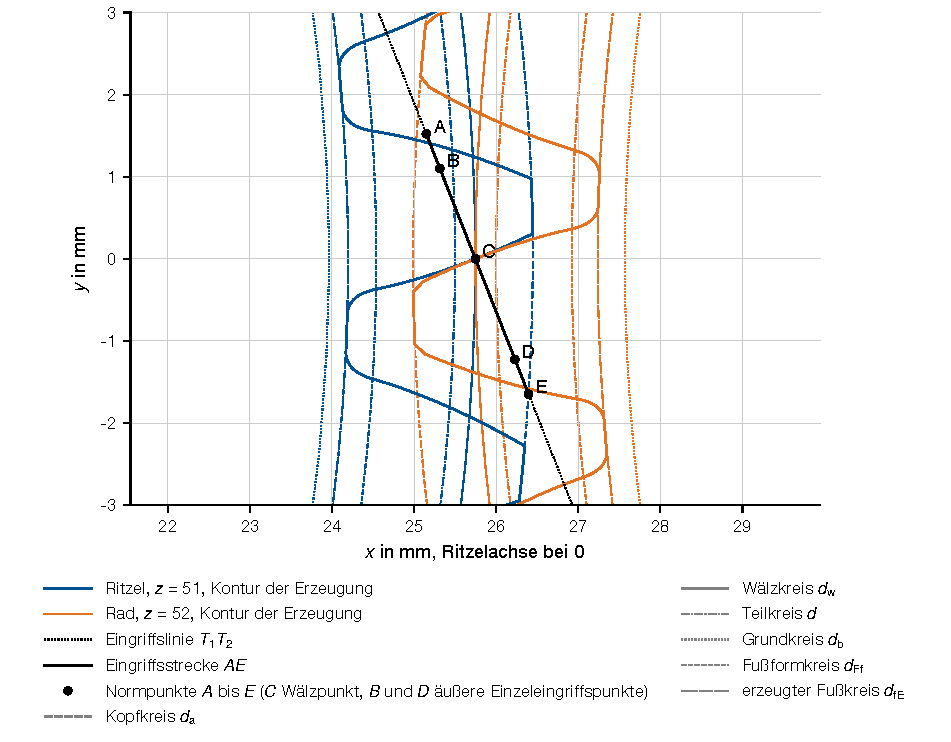
\includegraphics[width=0.9\textwidth]{kap3/stirnschnitt_kste}
    \caption{Stirnschnitt der Prüfverzahnung kst-E in der Stellung C: Konturen der Erzeugung, Kreise der Geometrietabelle, Eingriffslinie und Eingriffsstrecke mit den Normpunkten A bis E (das Ritzel treibt im Uhrzeigersinn, die rechten Flanken arbeiten).}
    \label{fig:stirnschnitt_kste}
\end{figure}

\begin{table}[htbp]
    \caption{Nenngeometrie der Prüfverzahnung kst-E nach dem STplus-Fall, ausgegeben durch die Geometriekette dieser Arbeit, und Werkstoffe nach den Zeichnungen.}
    \label{tab:geometrie_kste}
    \centering
    \begin{tabular}{llcc}
        Größe                               & Zeichen                              & Ritzel                         & Rad        \\
        \hline
        Zähnezahl                           & $z$                                  & $51$                           & $52$       \\
        Normalmodul in mm                   & $m_{\mathrm{n}}$                     & \multicolumn{2}{c}{$1{,}0$}                 \\
        Normaleingriffswinkel in °          & $\alpha_{\mathrm{n}}$                & \multicolumn{2}{c}{$20{,}000$}              \\
        Schrägungswinkel in °               & $\beta$                              & \multicolumn{2}{c}{$0$}                     \\
        Achsabstand in mm                   & $a_{\mathrm{w}}$                     & \multicolumn{2}{c}{$52{,}000$}              \\
        Profilverschiebungsfaktor           & $x$                                  & $0{,}2034$                     & $0{,}3143$ \\
        Zahnbreite in mm                    & $b$                                  & $17$                           & $15$       \\
        Teilkreisdurchmesser in mm          & $d$                                  & $51{,}000$                     & $52{,}000$ \\
        Grundkreisdurchmesser in mm         & $d_{\mathrm{b}}$                     & $47{,}924$                     & $48{,}864$ \\
        Wälzkreisdurchmesser in mm          & $d_{\mathrm{w}}$                     & $51{,}495$                     & $52{,}505$ \\
        Kopfkreisdurchmesser in mm          & $d_{\mathrm{a}}$                     & $52{,}894$                     & $54{,}022$ \\
        Fußformkreisdurchmesser in mm       & $d_{\mathrm{Ff}}$                    & $49{,}081$                     & $50{,}157$ \\
        erzeugter Fußkreisdurchmesser in mm & $d_{\mathrm{fE}}$                    & $48{,}394$                     & $49{,}524$ \\
        Kopfhöhenfaktor des Werkzeugs       & $h_{\mathrm{aP0}}/m_{\mathrm{n}}$    & $1{,}10$                       & $1{,}25$   \\
        Kopfrundungsfaktor des Werkzeugs    & $\rho_{\mathrm{aP0}}/m_{\mathrm{n}}$ & $0{,}20$                       & $0{,}20$   \\
        Fußformhöhenfaktor des Werkzeugs    & $h_{\mathrm{FfP0}}/m_{\mathrm{n}}$   & $1{,}30$                       & $0{,}8456$ \\
        Erzeugungsprofilverschiebungsfaktor & $x_{\mathrm{E}}$                     & $-0{,}203$                     & $0{,}012$  \\
        Zahnweite über $k = 6$ Zähne in mm  & $W_{\mathrm{k}}$                     & $17{,}090$                     & $17{,}180$ \\
        Zahnweitenabmaß in mm               &                                      & $-0{,}278$                     & $-0{,}207$ \\
        Betriebseingriffswinkel in °        & $\alpha_{\mathrm{wt}}$               & \multicolumn{2}{c}{$21{,}463$}              \\
        Profilüberdeckung                   & $\varepsilon_{\alpha}$               & \multicolumn{2}{c}{$1{,}154$}               \\
        Werkstoff nach Zeichnung            &                                      & 20MnCr5                        & PA46-GF30  \\
    \end{tabular}
\end{table}

Beide Räder sind im STplus-Fall über zahnstangenförmige Bezugsprofile erzeugt. Das Werkzeugprofil des Ritzels trägt eine Kopfhöhe von $1{,}10\,m_{\mathrm{n}}$ und einen Kopfrundungsradius von $0{,}20\,m_{\mathrm{n}}$. Die Zeichnung von 2022 schreibt dazu Profilschleifen vor. Für das Rad legt die Zeichnung die Zahnform über das Bezugsprofil eines Wälzfräsers mit $h_{\mathrm{aP0}} = 1{,}25$\,mm und $\rho_{\mathrm{aP0}} = 0{,}20$\,mm fest. Das Rad wird spritzgegossen, die Flanken bleiben ohne Nachbearbeitung. Die Fußrundung beider Räder ist die Trochoide der abgerundeten Werkzeugkopfkante zwischen dem Fußformkreis und dem erzeugten Fußkreis, am Rad also zwischen $50{,}157$\,mm und $49{,}524$\,mm. An der $30$°-Tangente weist die Ergebnisliste für das Rad einen bezogenen Fußrundungsradius von $0{,}38$ und eine Fußdickensehne von $2{,}197$\,mm aus, für das Ritzel $0{,}40$ und $2{,}068$\,mm. Die Kontur der Geometriekette dieser Arbeit gibt für das Rad dieselben Werte wieder (\figref{fig:zahnkontur_kste}). Am Kopf des Rades rechnet STplus mit einem Kantenbruch unter $45$° und einem Radialbetrag von $0{,}117$\,mm, während die Zeichnung eine Kopfrundung mit dem Radius $0{,}2$\,mm vorsieht. Mit den Zahnweitenabmaßen der Tabelle ergeben sich Zahnweiten von $16{,}812$\,mm am Ritzel und $16{,}973$\,mm am Rad. Die Zeichnungen schreiben als Fertigmaß $16{,}822$\,mm mit dem Abmaß $-0{,}021$\,mm und $17{,}002$\,mm mit dem Abmaß $-0{,}059$\,mm vor.

%\Note{PH: Abgleich aller Zeichnungsfelder gegen den STplus-Fall (M7a) steht aus; Tabelle der Unterschiede nachtragen.}

\begin{figure}[htbp]
    \centering
    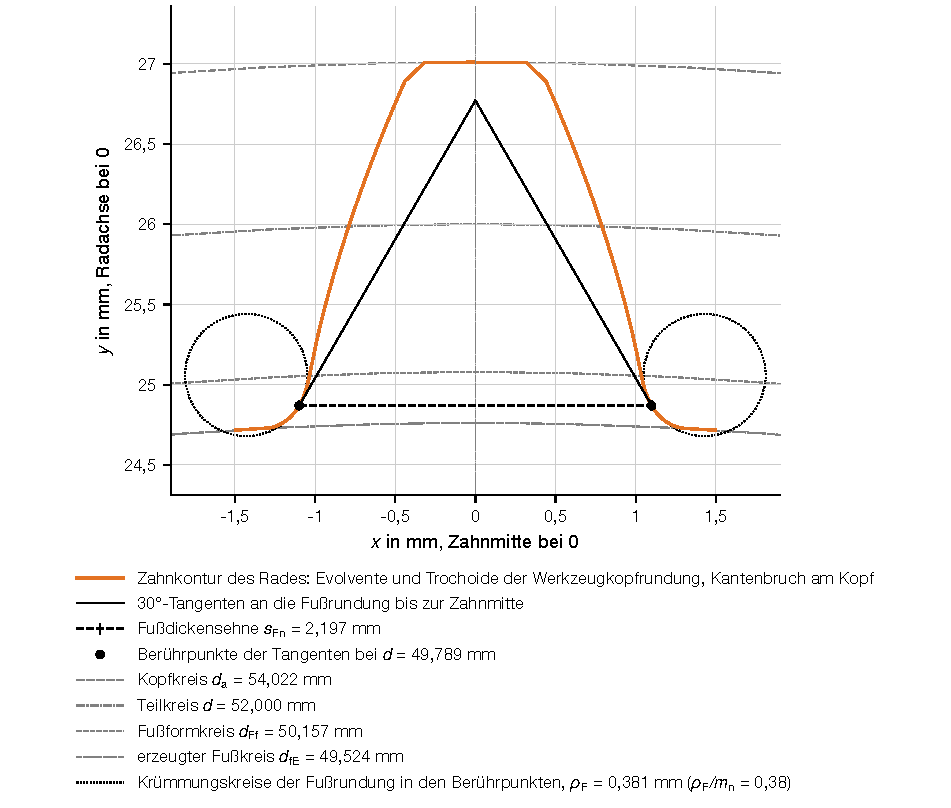
\includegraphics[width=0.85\textwidth]{kap3/zahnkontur_kste}
    \caption{Zahn des Rades kst-E im Stirnschnitt: Evolvente, Trochoide der Werkzeugkopfrundung und Kantenbruch, die Kreise der Erzeugung, die $30$°-Tangenten mit Fußdickensehne und Krümmungsradius aus der Kontur der Geometriekette.}
    \label{fig:zahnkontur_kste}
\end{figure}

Das Ritzel besteht nach beiden Zeichnungsständen aus dem Einsatzstahl 20MnCr5, der gasaufgekohlt und in Öl abgeschreckt wird. Gefordert sind eine Randhärte von $670$ + $100$\,HV\,1 und eine Einhärtetiefe von $0{,}3$ + $0{,}1$\,mm bei der Grenzhärte $550$\,HV\,1. Die Kernfestigkeit liegt zwischen $900$\,N/mm$^{2}$ und $1300$\,N/mm$^{2}$. Die Zeichnung von 2022 verlangt profilgeschliffene Flanken mit $R_{\mathrm{a}}$ von $0{,}20$\,\textmu m bis $0{,}25$\,\textmu m und eine Qualität besser als 6 nach DIN 3961 bis 3967. Dazu kommt eine lineare Kopfrücknahme $C_{\mathrm{a}} = 25$\,\textmu m ab dem Durchmesser $51{,}946$\,mm. Der Zeichnungsstand von 2025 beschreibt nur die Vorverzahnung mit einem Protuberanzfräser (Kopfhöhe $1{,}34\,m_{\mathrm{n}}$, Kopfrundung $0{,}25\,m_{\mathrm{n}}$) sowie geschliffene Bohrung und Planflächen. Die Endbearbeitung steht nicht auf der Zeichnung, weil sie in der Werkstatt des Lehrstuhls erfolgt. Dort werden die Flanken nachgeschliffen und die Kopfrücknahme eingebracht. In der Verzahnungsmessung zeigen die Prüfstandsritzel deshalb die Kopfrücknahme und die Zahnweite der Zeichnung von 2022 (\secref{sec:pruefraeder_vorher}). Im FE-Modell wird das Ritzel als Modellwahl ohne Kopfrücknahme nach der Nenngeometrie des STplus-Falls abgebildet (\secref{sec:fe_modell}). Im STplus-Fall selbst ist das Ritzel mit der Werkstoffkarte 16MnCr5 und das Rad mit einer Karte für PA66 belegt. Beide Karten dienen allein der Geometrie. Die Werkstoffdaten der Berechnung stammen aus den Zugversuchen in \secref{sec:fe_modell}.

Das Rad wird aus dem glasfaserverstärkten Polyamid 46 PA46-GF30 (Stanyl TW200F6 von Envalior) auf einen Stahleinleger gespritzt. Die Zeichnung des Rades nennt als Fertigung Spritzgießen und als Verzahnungsqualität Q10 nach DIN ISO 1328-1:2018-03. Die Bohrung 20 G6 mit der Passfedernut 6 J8 liegt im Einleger. Der Kunststoff ist in den Nuten des Einlegers eingespritzt und so gegen axiales Verschieben gesichert, das Rad sitzt über eine Passfeder auf der Welle \cite[S.~47]{Fie23}. Die Räder dieser Arbeit tragen dieselben Einleger aus 16MnCr5 wie die Räder der Laufversuche 2023. Der Kunststoffkörper beginnt beim Durchmesser $33$\,mm, die Nabe reicht in voller Breite bis zum Radius $19{,}107$\,mm. Von beiden Stirnseiten ist je eine $5{,}5$\,mm tiefe Tasche bis zum Radius $22{,}168$\,mm ausgespart. Ihre Wände stehen unter $93$° zur Stirnseite, so dass die Tasche mit der Tiefe schmaler wird. Drei der Ecken tragen den Radius $0{,}5$\,mm. Zwischen den Taschengründen bleibt ein Steg von $4$\,mm Dicke, außen trägt die Felge die Verzahnung über die volle Zahnbreite von $15$\,mm (\figref{fig:netz_koerper} in \secref{sec:fe_modell}). Für das Rad liegt ein Zeichnungsstand vor (Ausgabe 28.02.2022), für das Ritzel die Stände vom 08.06.2022 und vom 02.04.2025.

% gestrichen (TK kap3_6:87): Bild radkoerper_kste; der Radkörper steht nur noch in 3.6 als Bild netz_koerper, dort mit der z-Achse horizontal.

% TK erledigt (Bild hier gestrichen; netz_koerper in 3.6 mit z horizontal und weniger Maßen neu gezeichnet): Bitte die z-Achse auf die horizontale Ordinate, dann kann man sich den Zahnradkörper im Werschnitt besser vorstellen. Bitte weniger Radius und rundungsbemaßungen, die sind über die ordinaten ersichtlich, dann ist die Zeichnung auch aufgeräumter und überlappt nicht so stark. Entsprechend die Zeichnung überarbeiten.

Für die Laufversuche und die Messungen stehen 36 Räder und 8 Ritzel mit fünfstelligen Teilenummern der Stückliste zur Verfügung (\tabref{tab:teilegruppen_kste}). Zehn Räder bilden die Kerngruppe der eigenen Laufversuche auf dem Prüfstand KV3. Darunter diente 97351 dem Vorversuch zur Temperatur, und 97361 wurde nicht mehr gefahren, weil der Prüfstand nach dem Ausfall des Drehzahlsensors gewartet wird. Alle übrigen 26 vermessenen Räder bilden die Gruppe der Fertigungsstreuung. Dazu zählt das Rad 97364, das als zweites Rad der Stufe $8$\,Nm lief und von einer studentischen Hilfskraft vermessen wurde. Sieben Ritzel der Nummern 95911 bis 95920 gehören zur Serie, aus der das Prüfstandsritzel stammt. Sie wurden im Oktober 2025 vermessen. Das Ritzel 86481 ist ein älteres Stück mit einem Konturscan aus dem Jahr 2023. Sein Fußkreis liegt $0{,}17$\,mm unter dem der Serie, es ist anders geschnitten und dient nicht als Referenz. Der Zahn 1 ist auf den Teilen markiert und wird von Messmaschine, Konturscan und Prüfstand gleich gezählt. Die Laststufen je Teil stammen aus der Versuchsdatei des Prüfstands (\secref{sec:pruefstand}). Der Messumfang je Gruppe folgt in \secref{sec:dokumentation_pruefraeder}.

% TK erledigt (97351 Vorversuch, 97361 nicht gefahren, 97364 bei 8 Nm): Bitte den Absatz auf aktuellen Stand bringen

\begin{table}[htbp]
    \caption{Teilegruppen der Prüfräder kst-E nach den Teilenummern der Stückliste.}
    \label{tab:teilegruppen_kste}
    \centering
    \small
    \begin{tabular}{L{3.4cm}L{5.6cm}lL{4.4cm}}
        Gruppe                      & Teilenummern                                                         & Anzahl & Bemerkung                                                                          \\
        \hline
        Kernräder der Laufversuche  & 97340, 97345, 97346, 97350, 97351, 97355, 97360, 97361, 97365, 97366 & 10     & 97351 Vorversuch, 97361 ($8$\,Nm) aufgrund Prüfstandswartung noch nicht untersucht \\
        Fertigungsstreuung          & 97341 bis 97375 ohne Kernräder                                       & 26     & einschließlich 97364                                                               \\
        Zusatzversuch               & 97364                                                                & 1      & $8$\,Nm, zweites Rad der Stufe, zählt zur Streuung                                 \\
        Serie des Prüfstandsritzels & 95911, 95912, 95915, 95917, 95918, 95919, 95920                      & 7      & Verzahnungsmessung Oktober 2025                                                    \\
        älteres Ritzel              & 86481                                                                & 1      & Konturscan 2023                                                                    \\
    \end{tabular}
\end{table}

% Bildwunsch: Stirnschnitt der Paarung mit Bezeichnungen (Teil-, Grund-, Wälz-, Kopf-, Fußform- und Fußkreis,
%   Eingriffslinie, Normpunkte A bis E), Label fig:stirnschnitt_kste (eigene Zeichnung aus der Geometriekette, T5).
% Bildwunsch: Zahnkontur des Rades mit Fußrundung (Trochoide), Fußformkreis und 30-Grad-Tangente, Label
%   fig:zahnkontur_kste (T5-Skript).
% Bildwunsch: Radkörperschnitt (Meridianhalbschnitt durch die Zahnmitte: Einleger, Nabe, Taschen, Steg, Felge, Maße),
%   Label fig:radkoerper_kste (eigene Zeichnung T5 nach 90_CAD/Schnitt_Symmetrie_Zahnradkoerper_mit_Zahn.png).

% Herkunft:
% Absatz 1: Achsabstand 52 mm und Prüfstand: 00_gliederung.md Zeile 3.2; MA-0296.txt (pdftotext) Z. 1672 (PDF S. 52);
%   Benennung kst-E: MA-0296 Abschnitt 4.2, PDF S. 55 (gedruckt S. 42), Verweis auf [Rei22] PDF S. 59 (gedruckt S. 46);
%   Ritzel treibt: kst-E_eingabe.ste RAD_1_TREIBT; Referenzpaar "verified": scripts/oracle_cases.yaml Fall kst_e;
%   Ergebnisliste 11.0F vom 14.02.25: kst-E-ausgabe.sta Blatt 1; α_wt 21,463°, ε_α 1,154: gearcore-Ausgabe
%   (compute_generation_from_data) und .sta Blatt 6.
% Tabelle 1 (Zeile für Zeile): z, m_n, α_n, β, a, x, b, d_a, W_k, Abmaße: kst-E_eingabe.ste Zeilen 5 bis 17 und
%   .sta Blatt 6/7; d, d_b, d_w: gearcore-Ausgabe (reference, base, working pitch diameter) = .sta Blatt 6;
%   d_Ff 49,081/50,157 und d_fE 48,394/49,524: gearcore root_form_diameter_mm, generated_root_diameter_mm
%   (STplus druckt einfachgenau 50,158 und 49,523); Werkzeugfaktoren: .ste Blöcke WKZ_Profil_B_Ritzel/_Rad und
%   .sta Blatt 7/8 (h_FfP0* 1,300 für das Ritzel vom Programm belegt, gearcore root_form_height_factor 1.3);
%   x_E: gearcore −0,2032/0,0121, .sta Blatt 8 −0,2030/0,0117 (auf drei Stellen gleich);
%   α_wt, ε_α: s. o.; Werkstoff nach Zeichnung: 20220623/20250402 (20MnCr5), parts.yaml (PA46-GF30).
% Absatz 2: Bezugsprofile und Profilschleifen: .ste; Zeichnung Ritzel 20220623 (Flankenbearbeitung Profilschleifen,
%   haP0 1,10 mn, rhoaP0 0,20 mn); Zeichnung Rad 20220316 (Werkz.-Profil Wälzfräser, haP0 1,25 mm, rho_aP0 0,20 mm,
%   Spritzgegossen, keine Nachbearbeitung); Fußrundung Fußformkreis bis Fußkreis: gearcore-Werte s. Tabelle;
%   30-Grad-Tangente rho_F* 0,40/0,38, s_fn* 2,068/2,197: .sta Blatt 11; Kantenbruch 45° und h_K 0,117 mm: .sta Blatt 6
%   und 9; Kopfrundung r 0,2 mm: Zeichnung Rad 20220316; Zahnweiten 16,812/16,973 mm: ADR-117 Amendment 2026-10-12
%   Punkt 1 und 3 (architecture_decisions.md Z. 2086 und 2101); Fertigmaße: Zeichnung Ritzel 20220623 (16,822 −0,021),
%   Zeichnung Rad 20220316 (17,002 −0,059); M7a offen: implementation_roadmap.md Z. 129.
% Absatz 3: Werkstoff, Wärmebehandlung, Härte, Einhärtetiefe, Kernfestigkeit, Ra, Qualität, Kopfrücknahme 25 µm ab
%   51,946 mm: Zeichnung Ritzel 20220623; Protuberanzfräser 1,34 mn / 0,25 mn, Bohrungs- und Planflächenschleifen, kein
%   Zahnflankenschleifen: Zeichnung Ritzel 20250402; Endbearbeitung (Nachschleifen der Flanken und Kopfrücknahme) in
%   der Werkstatt des Lehrstuhls, nicht auf der Zeichnung: Angabe des Nutzers, Kommentar in dieser Datei 2026-10-17;
%   Prüfstandsritzel zeigen Rücknahme und Zahnweite 2022: ADR-116
%   Punkt 44 (architecture_decisions.md Z. 1536 bis 1539), ADR-118 Punkt 8 (Z. 2217 bis 2222); FE-Ritzel ohne
%   Rücknahme nach STplus-Nenngeometrie: ADR-116 Punkt 44 (Z. 1543 bis 1544, "base geometry stays"), .ste
%   OHNE_RUECKNAHME = ja;
%   Werkstoffkarten 16MnCr5 / PA66: .ste WERKSTOFF; Zugversuche als Werkstoffquelle: ADR-118 Kontext (Z. 2169 bis 2171).
% Absatz 4: PA46-GF30 Stanyl TW200F6 (Envalior): parts.yaml (material), ADR-119 Kontext (Z. 2701), sources.yaml
%   CAMPUS-StanylTW200F6:2024; Spritzgießen, Q10 DIN ISO 1328-1:2018-03, Bohrung 20 G6, Nut 6 J8, Stahleinleger:
%   Zeichnung Rad 20220316; Nuten des Einlegers, Passfeder, Einleger 16MnCr5 (Räder 2023): MA-0296 PDF S. 59/60
%   (gedruckt S. 46/47); Radkörpermaße (Bohrung 33 mm, Nabe r 19,107, Tasche 5,5 tief bis r 22,168, 93°, R 0,5,
%   Steg 4 mm, b 15): data/fe/body_sections.yaml und 80_output/fe/kst_e/frozen_mesh_20layers_bore33_pocket/README.md
%   Absatz 2; Zeichnungsstände: Ausgabedaten auf den drei Zeichnungen (28.02.2022, 08.06.2022, 02.04.2025).
% Absatz 5 und Tabelle 2: Gruppen, Teilenummern, Einlauf 97351, 97361 läuft (8 Nm), 97364 Zusatzversuch 12 Nm durch
%   Hilfskraft, Serie 95911 bis 95920 (GINA Oktober 2025), 86481 nur Konturscan 2023, Zahn 1 markiert:
%   data/measurement/parts.yaml (provenance.notes, groups, labels); Zählung 44 Teile = 10 + 26 + 7 + 1:
%   80_output/messungen/inventory/inventory.md Kopf und Zähltabellen, ADR-117 Consequences (Z. 1998 bis 1999);
%   86481 Fußkreis 0,17 mm unter der Serie, anders geschnitten, keine Referenz: ADR-117 Amendment 2026-10-12
%   Punkt 4 (Z. 2131 bis 2133); Laststufen aus der Prüfstandsdatei: parts.yaml provenance.notes.
% Nomenklatur: alpha_wt (Betriebseingriffswinkel), x_E (Erzeugungsprofilverschiebungsfaktor), h_FfP0
%   (Fußformhöhe des Werkzeug-Bezugsprofils) fehlen noch in Nomenklatur.tex; d_f der Zeichnungen wird im Text
%   nicht als Symbol verwendet, der erzeugte Fußkreis steht als d_fE.


\section{Prüfstand und Versuchsdurchführung}
\label{sec:pruefstand}

Die Laufversuche dieser Arbeit wurden auf einem FZG-Kleinverspannungsprüfstand mit dem Achsabstand $52$\,mm gefahren. In der Semesterarbeit SA 1272 wurden zwei vorhandene Kleingetriebeprüfstände dieses Achsabstands für Laufversuche an nitrierten Zahnrädern mit dem Normalmodul $2$\,mm umkonstruiert. Der Grundaufbau folgt dem Verspannungsprüfstand der FZG in seiner Standardbauart, die nach Schurer in DIN 51354 genormt ist \cite[S.~2 und 8]{Schu09}. Übertragungsgetriebe und Prüfgetriebe sind über zwei Torsionswellen zu einem geschlossenen Leistungskreislauf verbunden. Das Prüfmoment entsteht durch Verdrehen und Verspannen der beiden Hälften einer Verspannkupplung und ist dem Verdrehweg proportional. Aufgebracht wird es mit einer Verspannschere oder mit einem Belastungshebel samt Gehänge und Gewichten. Der Motor speist nach dem Anlauf nur die Verlustleistung in den Kreislauf ein, die Ölversorgung übernimmt ein drucküberwachtes Ölaggregat, und ein Rohrheizkörper mit Schaltthermometer im Prüfgetriebekasten regelt die Schmierstofftemperatur \cite[S.~8]{Schu09}.

\figref{fig:pruefstand_sa1272} zeigt das Konstruktionsmodell des Prüfstands. Ein Servomotor mit einem Nennmoment von $7{,}6$\,Nm, mit Fremdlüfter etwa $12$\,Nm, treibt über eine Elastomerkupplung die Ritzelwelle des Übertragungsgetriebes. Dessen schrägverzahnte Räder übertragen die Leistung mit dem Zähnezahlverhältnis 29/21 auf die Radseite \cite[S.~9 und 48]{Schu09}. Die Radwelle des Übertragungsgetriebes läuft durch einen Lagerbock und ist über eine Kupplungshülse mit der Radwelle des Prüfgetriebes verbunden. Im Prüfgetriebe sitzen beide Wellen in einer Fest-Los-Lagerung aus Zylinderrollenlagern, und eine abnehmbare Frontplatte erlaubt den Wechsel der Prüfverzahnung \cite[S.~9 und 42]{Schu09}. Die Ritzelwelle des Prüfgetriebes führt in die Verspannkupplung, die wegen des kleineren Moments auf der Ritzelseite angeordnet ist und mit zwölf Verspannschrauben für $120$\,Nm am Ritzel ausgelegt wurde \cite[S.~46]{Schu09}. Zwischen Verspannkupplung und Übertragungsgetriebe liegt die Drehmomentmesswelle, die das Drehmoment mit Dehnungsmessstreifen erfasst und daneben Drehzahl und Wellenwinkel ausgibt; eine Balgkupplung bindet sie an die Ritzelwelle des Übertragungsgetriebes an \cite[S.~10 und 52]{Schu09}. Eine speicherprogrammierbare Steuerung im Schaltschrank steuert Prüfstand und Ölaggregat und gibt die Messwerte aus \cite[S.~53]{Schu09}. Als Prüfverzahnung sah die SA 1272 Stirnräder aus Nitrierstahl mit dem Normalmodul $2$\,mm bei den Zähnezahlen 21 und 29 vor; die Zahnbreite betrug $8$\,mm \cite[S.~42]{Schu09}. In dieser Arbeit läuft auf demselben Achsabstand die Prüfverzahnung kst-E mit dem Normalmodul $1$\,mm (\secref{sec:pruefverzahnung}). \Note{PH: Prüfstandsfoto.}

\begin{figure}[htbp]
    \centering
    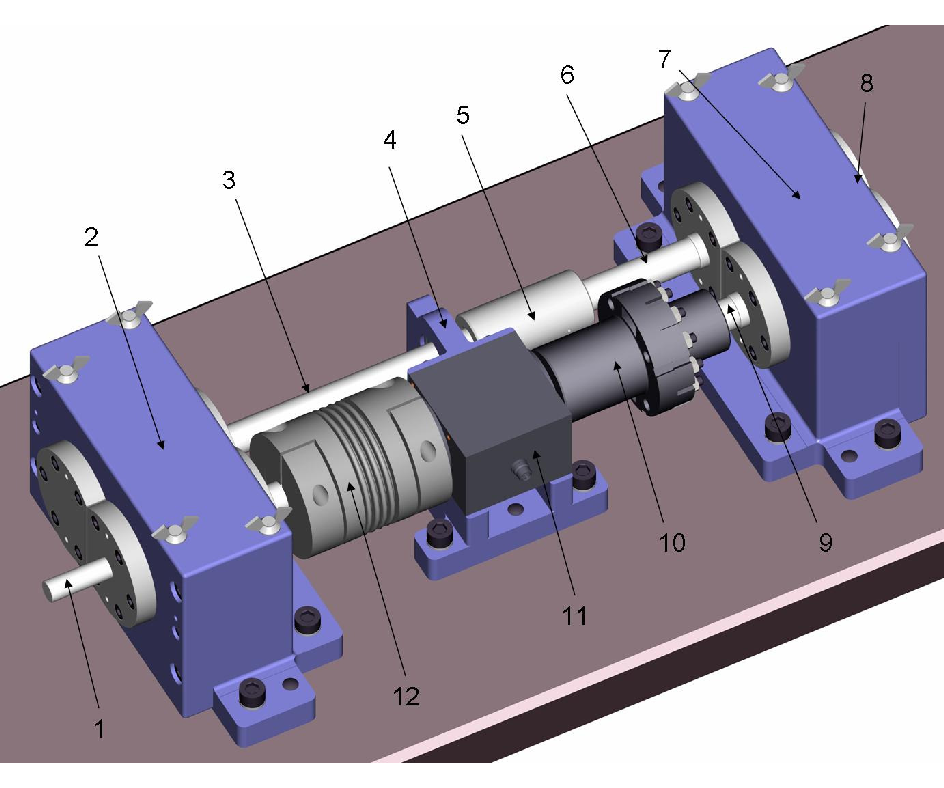
\includegraphics[width=0.8\textwidth]{kap3/quelle_pruefstand_sa1272}
    \caption{Verspannungsprüfstand mit dem Achsabstand $52$\,mm als Konstruktionsmodell: Ritzelwelle (1) und Übertragungsgetriebe (2), Radwelle (3) mit Lagerbock (4), Kupplungshülse (5), Radwelle (6) des Prüfgetriebes (7) mit Frontplatte (8), Ritzelwelle (9), Verspannkupplung (10), Drehmomentmesswelle (11) und Balgkupplung (12) auf der Grundplatte, nach \cite[S.~9]{Schu09}.}
    \label{fig:pruefstand_sa1272}
\end{figure}

Die Prüfbedingungen der Laufversuche an der kst-E-Verzahnung wurden für die Versuche des Jahres 2023 festgelegt \cite[S.~39 und 40]{Fie23}. Das Öl wird über Einlässe in den Deckeln der Getriebekästen zwischen die Zahnflanken eingespritzt und aus einer Bohrung im Kastenboden in den Kreislauf zurückgepumpt \cite[S.~10]{Schu09}; die Durchflussrate betrug $4{,}0$\,l/min. Schmierstoff ist das FVA-Referenzöl FVA 3A, ein Mineralöl der Viskositätsklasse ISO VG 100 mit $4$\,\% Anglamol 99. Die Prüfräder werden über den Schmierstoff temperiert, damit sich eine Zahnmassentemperatur von $80$\,°C einstellt. VDI 2736 Blatt 4 lässt bei Ölschmierung die Öltemperatur als Näherung für die Zahnfußtemperatur zu \cite[S.~16]{VDI2736-4}. Das Verspannmoment misst eine Drehmomentmesswelle burster 8651-5050-V0022 mit dem Messbereich bis $50$\,Nm im Verspannkreis. Auf der Welle sitzt das Kunststoffrad über eine Passfeder und ist mit einem Querpressverband gesichert, wozu der Lagerinnenring erwärmt und auf die mit Kältespray gekühlte Welle geschoben wird. Als Gegenrad diente 2023 ein einsatzgehärtetes Ritzel aus 16MnCr5 mit $20$\,\textmu m Kopfrücknahme \cite[S.~40]{Fie23}; das Ritzel dieser Arbeit ist in \secref{sec:pruefverzahnung} beschrieben.

Gegenüber den Versuchen 2023 blieben die Verzahnung, der Schmierstoff, die Einspritzschmierung und die Zieltemperatur von $80$\,°C unverändert. Die Versuche 2023 liefen auf dem Prüfstand KV4 mit dem Ritzel 86481 bei $2250$\,1/min. Für diese Arbeit läuft der Prüfstand KV3 mit dem Ritzel 95919 bei $3058$\,1/min am Ritzel, also $3000$\,1/min am Rad. \Note{PH: Zuordnung von KV3 und KV4 zu den beiden Exemplaren nach SA 1272 sowie Messwelle und Ölaggregat des KV3 bestätigen.} Während des Laufs kst-E\_72 wurde der Ölfilter gereinigt und der Durchfluss an einer neuen Düse auf $1{,}5$\,l/min eingestellt. \Note{PH: Öldurchfluss der Läufe 2026 vor dem Düsenwechsel.} Die Temperaturregelung bezieht sich auf den Prüfkasten, während das Ölaggregat im Dauerbetrieb etwa $10$\,K wärmer läuft; deshalb wird das Moment erst eingestellt, wenn sich beide Temperaturen angeglichen haben.

VDI 2736 Blatt 4 verlangt für die Ermittlung von Tragfähigkeitskennwerten Laufversuche bei festgehaltener Werkstofftemperatur, konstanter Drehzahl und konstantem Drehmoment bis zum Versagen des Bauteils \cite[S.~6]{VDI2736-4}. Je Paar aus Drehmoment und Temperatur sind mindestens drei Wiederholungen vorzusehen, für eine Temperatur mindestens vier Drehmomente \cite[S.~6 und 7]{VDI2736-4}. Die Versuche 2023 wurden als einstufige Wöhlerversuche auf drei Lastniveaus mit mindestens drei Versuchspunkten gefahren \cite[S.~65]{Fie23}. Dem folgt der Versuchsplan dieser Arbeit in \tabref{tab:versuchsplan}. Die Lasthorizonte sind als Radmoment $T_{\mathrm{2}}$ mit $8$\,Nm, $12$\,Nm und $16$\,Nm festgelegt; am Ritzel entspricht das über das Zähnezahlverhältnis 51/52 den Momenten $7{,}85$\,Nm, $11{,}8$\,Nm und $15{,}7$\,Nm. Als Drehzahl sind $3058$\,1/min am Ritzel eingestellt, als Öltemperatur $75$\,°C; die Zieltemperatur der Zähne beträgt $80$\,°C. Nach dem Wechsel des Temperatursensors am Prüfkasten und der Düse steht für die Läufe ab kst-E\_70 ein Sollwert von $67$\,°C in der Arbeitsmappe. Von den zehn Rädern der Kerngruppe diente 97351 dem Vorversuch kst-E\_63. Die übrigen neun Räder belegen die Horizonte: zwei Läufe bei $8$\,Nm (kst-E\_69, 75), drei bei $12$\,Nm (kst-E\_66, 68, 74) und vier bei $16$\,Nm (kst-E\_70 bis 73). \Note{PH: Rad des Laufs kst-E 75, Arbeitsmappe 97364 gegen Teileliste 97361.} \Note{PH: Stichtag der Laufversuche.}

\begin{table}[htbp]
    \caption{Versuchsplan der Laufversuche an der Prüfverzahnung kst-E nach der Arbeitsmappe des Prüfstands: Lasthorizonte dieser Arbeit (PA46-GF30, Prüfstand KV3, Ritzel 95919) sowie die Vergleichsläufe aus POM und PEEK auf demselben Horizont, 2026 auf demselben Prüfstand und 2023 auf dem Prüfstand KV4 (Ritzel 86481, $2250$\,1/min, Ritzelmoment $8$\,Nm, $12$\,Nm und $16$\,Nm, am Rad um 52/51 höher). Anzahl der Läufe PA46-GF30 als abgeschlossen/laufend mit den Teilenummern der Räder.}
    \label{tab:versuchsplan}
    \centering
    \footnotesize
    \setlength{\tabcolsep}{4pt}
    \begin{tabular}{L{1.6cm}L{1.6cm}L{1.5cm}L{1.6cm}L{2.3cm}L{1.1cm}L{1.1cm}L{1.1cm}L{1.1cm}}
        Moment Rad in Nm & Moment Ritzel in Nm & Drehzahl Ritzel in 1/min & Öl\-tempe\-ratur in °C & PA46-GF30 (Räder) & POM 2026 & PEEK 2026 & POM 2023 & PEEK 2023 \\
        \hline
        $8$  & $7{,}85$ & $3058$ & $74$ bis $75$ & 1/1 (97345, 97364) & 0 & 0 & 1 & 0 \\
        $12$ & $11{,}8$ & $3058$ & $74$ & 3/0 (97350, 97360, 97365) & 0 & 0 & 3 & 2 \\
        $16$ & $15{,}7$ & $3058$ & $67$ & 4/0 (97340, 97346, 97355, 97366) & 3 & 0 & 4 & 4 \\
        $8$, $12$, $16$ (Vorversuch) & $7{,}85$ bis $15{,}7$ & $2294$ und $3058$ & $75$ & 1/0 (97351) & & & & \\
    \end{tabular}
\end{table}

Der Vorversuch kst-E\_63 am Rad 97351 bestand aus einer Temperaturmatrix. Die drei Momente wurden mit den Drehzahlen $2294$\,1/min und $3058$\,1/min am Ritzel, also $2250$\,1/min und $3000$\,1/min am Rad, für je $2$\,h gefahren. Am Ende jeder Stufe wurde die Zahnflankentemperatur mit einem Infrarotthermometer bei dem Emissionsgrad $1$ gemessen. VDI 2736 Blatt 4 verlangt für optische Messungen den Emissionsgrad des Kunststoffs aus Voruntersuchungen und weist die Zuverlässigkeit des Verfahrens für Stirnräder als nicht nachgewiesen aus \cite[S.~17 und 18]{VDI2736-4}. Die Messwerte dienen deshalb dem Bezug auf die Zahnmassentemperatur von $80$\,°C in \secref{sec:temperatur} und nicht als Kennwert. Anschließend lief das Rad bei $3058$\,1/min bis zum Versagen weiter.

Jeder Lauf beginnt mit dem Verspannen im Stillstand. Das Moment wird mit dem Belastungshebel und Zusatzmassen an der Verspannkupplung aufgebracht, an der Messwelle abgelesen und mit einer Madenschraube gesichert. Der statische Wert liegt über dem Moment, das sich nach dem Start im Lauf einstellt. Eingetragen werden das Moment nach dem Start, nach $15$\,min und nach $60$\,min sowie der Stand des Lastwechselzählers der Steuerung. Fällt das Moment durch Verschleiß und Verformung der Kunststoffzähne ab, wird nachgespannt; VDI 2736 Blatt 4 fordert hierfür die Überwachung des Verspannmoments mit einer Drehmomentmessung \cite[S.~11]{VDI2736-4}. Bei den ersten Läufen geschah das bei Abfällen von etwa $1$\,Nm bis $3$\,Nm, teils mit Werten über dem Sollmoment. Ab dem Lauf kst-E\_74 gilt die Regel, nach $1$\,Nm Abfall auf höchstens $5$\,\% über dem Sollmoment nachzuspannen. Jedes Nachspannen wird mit Lastwechselzahl und Moment sowie den Temperaturen in der Spalte Bemerkung festgehalten, dazu der Befund einer Sichtprüfung der markierten Messzähne mit Fotos. Ein Lauf endet mit dem Zahnfußbruch, dessen Zahnnummer vermerkt wird, oder er läuft zum Stichtag noch.

Als Abbruchkriterium gilt der Totalausfall der Verzahnung, bei dem der Antrieb verloren geht. In den Versuchen 2023 zeigte POM ein schleichendes Risswachstum ohne eindeutigen Ausfallzeitpunkt \cite[S.~65]{Fie23}. Deshalb wurde dort zusätzlich ein Abfall des Drehmoments von mehr als $1$\,Nm über $100\,000$ Lastwechsel als Ausfall definiert, weil ab dieser Grenze keine zuverlässige Drehmomentübertragung mehr möglich ist. Dieses Ersatzkriterium wird in der Arbeitsmappe ab dem Lauf kst-E\_74 ausdrücklich übernommen. Ein zunehmendes sinusförmiges Laufgeräusch ist in den Bemerkungen als Vorzeichen des Bruchs festgehalten.

Auf demselben Prüfstand und mit demselben Ritzel fuhr die Betreuerin 2026 Vergleichsläufe mit Rädern aus POM und PEEK (kst-E\_50 bis 62, 64, 65, 67). Bei $3058$\,1/min und $75$\,°C Öltemperatur liegen drei POM-Läufe bei $16$\,Nm und drei bei $10$\,Nm am Rad, dazu drei PEEK-Läufe bei $14$\,Nm und vier bei $18$\,Nm. Drei weitere POM-Läufe bei $8$\,Nm liefen trocken bei Raumtemperatur und $1945$\,1/min und stehen außerhalb des Plans. \Note{PH: PEEK-Typ der Läufe 2026.} Die Läufe 2023 (kst-E\_1 bis 45) wurden auf dem Prüfstand KV4 mit dem Ritzel 86481 bei $2250$\,1/min mit Rädern aus POM (Delrin 100NC010) und PEEK (Vestakeep 4000G) gefahren \cite[S.~43 und 65]{Fie23}. Dort sind die Lastniveaus als Ritzelmoment von $8$\,Nm bis $18$\,Nm festgelegt und liegen am Rad um das Verhältnis 52/51 höher. Den Ritzelmomenten $8$\,Nm, $12$\,Nm und $16$\,Nm entsprechen am Rad $8{,}16$\,Nm, $12{,}2$\,Nm und $16{,}3$\,Nm. In den Vergleich gehen die Läufe bei $73$\,°C bis $76$\,°C Öltemperatur und $2250$\,1/min ein. Außerhalb bleiben die ersten sieben Läufe mit $45$\,°C Öltemperatur, zwei Stufenläufe, die Läufe bei $1000$\,1/min bis $4000$\,1/min sowie die ohne Rad eingetragenen Zeilen.

% Herkunft:
% Absatz 1 (Prüfstand, Prinzip): SA-1272.txt S. 2 (Aufgabenstellung: zwei vorhandene Kleingetriebeprüfstände a = 52 mm,
%   Grundaufbau wie Standard-FZG-Verspannungsprüfstand), S. 8 (DIN 51354, geschlossener Leistungskreislauf, zwei
%   Torsionswellen, Verspannkupplung, Verdrehweg proportional, Verspannschere oder Belastungshebel mit Gehänge und
%   Gewichten, Motor speist Verlustleistung, drucküberwachtes Ölaggregat, Rohrheizkörper mit Schaltthermometer, zwei
%   Modelle gefertigt). Druckseite = PDF-Seite.
% Absatz 2 (Bauteile): SA-1272 S. 9 (Bild 2, Nummern 1 bis 10, Motor ca. 12 Nm, Elastomerkupplung, i = 29/21, Lagerbock,
%   Kupplungshülse, Frontplatte, Verspannkupplung mit Verspannschere), S. 10 (Messwelle 11, dämpfende Kupplung 12,
%   Grundplatte 13, Einspritzung über Einlässe in den Deckeln, Bohrung im Boden), S. 42 (4.3.4 Tabelle 1: a = 52, z 21/29,
%   mn 2, b 8, Nitrierstähle 31CrMoV9 und 15CrMoV5.9; 4.3.5 Fest-Los-Lagerung, Zylinderrollenlager), S. 43 (NUP204/NU204),
%   S. 44 bis 46 (Verspannkupplung zweiteilig, Verspannschrauben, auf der Ritzelseite, 12 Schrauben, 120 Nm am Ritzel),
%   S. 48 (KEB-Servomotor D3.SM.000.4400, 7,6 Nm bei 4000 1/min, mit Fremdlüfter ca. 12 Nm), S. 51 (Balgkupplung R&W
%   BKH150/95), S. 52 (Burster-Messwelle 100 bzw. 200 Nm, DMS, Drehzahl und Wellenwinkel, auf dem Lagerbock), S. 53
%   (Schaltschrank, SPS Simatic S7-300 steuert Ölaggregat und Prüfstand, Messwerterfassung). Modul 1 mm heute: Verweis
%   auf sec:pruefverzahnung.
% Absatz 3 (Prüfbedingungen 2023): MA-0296.txt Z. 1913 bis 1961 (PDF S. 52/53 = Druckseiten 39/40, Seitenoffset 13):
%   a = 52,0 mm, Öldurchfluss 4,0 l/min, burster 8651-5050-V0022 bis 50 Nm, Einspritzschmierung, Temperierung über
%   den Schmierstoff auf 80 °C Zahnmassentemperatur, Ritzel 16MnCr5 einsatzgehärtet mit 20 µm Kopfrücknahme,
%   Querpressverband (Passfeder, Lagerinnenring erhitzt, Welle mit Kältespray gekühlt), FVA 3A = FVA-Referenzöl Nr. 3,
%   ISO VG 100, 4 % Anglamol 99 (Tabelle 3). Öltemperatur als Näherung der Zahnfußtemperatur: VDI2736-4.txt Z. 1056
%   bis 1062, Abschnitt 8.2.2, Druckseite 16 (vor dem Kopf "– 17 –" in Z. 1082).
% Absatz 4 (gleich/anders): kst-E_Laufversuche_KV3.xlsx Blatt Tabelle1: Spalten Prüfstand (KV4 Zeilen 2 bis 52, KV3 ab
%   Zeile 53), ME-Nr. Ritzel (86481 bei 2023, 95919 bei 2026), Drehzahl (2250 bei 2023, 3058 bei den Läufen 2026 ab
%   kst-E_53); 3058 · 51/52 = 2999,1 1/min; Ölfilter gereinigt und 1,5 l/min an neuer Düse: Bemerkung kst-E_72 (Zeile 94);
%   Prüfkastentemperatur gegen Aggregattemperatur etwa 10 K, Moment erst nach dem Angleichen einstellen: Bemerkung
%   kst-E_71 (Zeile 93). KV4 auch in MA-0296 Druckseite 84 (Z. 3325) genannt.
% Absatz 5 (Versuchsplanung): VDI2736-4.txt Z. 365 bis 371 (Abschnitt 3, Druckseite 6: festgehaltene Materialtemperatur,
%   konstante Drehzahl, konstantes Drehmoment, Lastwechsel bis zum Versagen), Z. 380 bis 386 (3.1, S. 6: mindestens eine
%   Temperatur, mindestens vier Drehmomente, Block mit mindestens drei Wiederholungen), Z. 449 bis 455 (3.3, S. 7, n_wi >= 3);
%   dasselbe in Abschnitt 4, Z. 562 bis 568 (Druckseite 9, Kopf "– 9 –" in Z. 557), im Text nicht zitiert; MA-0296 Druckseite 65 (Z. 2780
%   bis 2786: einstufige Wöhlerversuche, 3 Lastniveaus mit mindestens 3 Versuchspunkten). Horizonte: xlsx Spalte
%   "Ziel Drehmoment Ritzel" 7,9 bzw. 7,8 / 11,8 / 15,7 Nm und Spalte "Drehmoment Rad" = Ritzel · 52/51 (8,05 bzw. 7,95 /
%   12,03 / 16,01 Nm); nachgerechnet 8 · 51/52 = 7,846, 12 · 51/52 = 11,769, 16 · 51/52 = 15,692 Nm. Drehzahl 3058,
%   Öltemperatur 75 (kst-E_63, 75), 74 (66, 68, 69, 74), 67 (70 bis 73), Ziel/Zahntemperatur 80: Zeilen 77 bis 95.
%   Sensorwechsel: letzte Spalte der Zeilen 91 bis 94 ("Durch Änderung des Temperatursensors beim Prüfkasten, andere
%   Düse, und womöglich zu wenig Volumenstrom"). Belegung: Zeile 77 kst-E_63 97351; 88 kst-E_66 97350 (12 Nm);
%   90 kst-E_68 97365 (12); 91 kst-E_69 97345 (8); 92 kst-E_70 97346 (16); 93 kst-E_71 97366 (16); 94 kst-E_72 97355
%   (16); 95 kst-E_73 97340 (16); 96 kst-E_74 97360 (12); 97 kst-E_75 97364 (8, Lastwechsel leer, läuft).
%   Kerngruppe: parts.yaml groups.core (97340, 97345, 97346, 97350, 97351, 97355, 97360, 97361, 97365, 97366).
% Tabelle: Zahlen wie Absatz 5; Vergleichsläufe 2026 (Zeilen 53 bis 89): POM kst-E_54, 55, 56 bei 15,7/16,0 Nm, 3058,
%   75 °C; POM kst-E_53, 57, 67 bei 9,8/10,0 Nm; PEEK kst-E_61, 62, 65 bei 13,73/14,0 Nm; PEEK kst-E_58, 59, 60, 64 bei
%   17,7 bzw. 17,65/18,0 Nm; POM kst-E_50, 51, 52 bei 7,9/8,05 Nm trocken, RT, 1945 1/min (ausgeschlossen); Zeilen 72
%   bis 75 sind Doppeleinträge der Läufe 58 bis 61 ("Daten verlieren wegen Problem von Rechner"), nicht gezählt.
%   Vergleichsläufe 2023 (Zeilen 2 bis 46, Ritzelmoment = Spalte "Ziel Drehmoment Ritzel", Rad = · 52/51):
%   8 Nm POM kst-E_40; 12 Nm POM kst-E_14, 15, 21 und PEEK kst-E_24, 42 (kst-E_30 vorzeitig abgebrochen,
%   "weiterführbar", ohne Lastwechsel, nicht gezählt; kst-E_22 Stufenlauf, nicht gezählt); 16 Nm POM kst-E_12, 19, 20, 29
%   (29 ohne Drehzahleintrag) und PEEK kst-E_11, 25, 26, 37 (kst-E_43 Stufenlauf, nicht gezählt; kst-E_6 bei 45 °C
%   Öl, nicht gezählt). Ausgeschlossen: kst-E_1 bis 7 (Öl 45 °C), 28/32/33/34/35/39 (3000, 4000, 1000 1/min),
%   44/45 (ohne Datum und Rad). 8 · 52/51 = 8,157, 12 · 52/51 = 12,235, 16 · 52/51 = 16,314 Nm.
% Absatz 6 (Vorversuch): xlsx Zeilen 77 bis 83 (kst-E_63, 97351: 11,8/2294, 11,8/3058, 7,9/2294, 7,8/3058, 15,7/2294,
%   15,7/3058, jeweils "nach 2h ... Zahnflankentemperatur mit Emissionsgrad 1 (nach Test von Liang)"; Zeile 83:
%   Weiterlauf bei 3058 bis "5-6 kaputte Zähne"); 2294 · 51/52 = 2249,9 1/min. Emissionsgrad und Zuverlässigkeit:
%   VDI2736-4.txt Z. 1097 bis 1123 (8.2.4, Druckseite 17) und Z. 1145 bis 1148 (Druckseite 18). Temperaturwerte selbst
%   nicht genannt (Kapitel 4.5, Label sec:temperatur aus kap4_voruntersuchungen.tex).
% Absatz 7 (Ablauf): xlsx Spalten "verspannt", "Drehmoment Ritzel T_0 nach Start", "15 min", "T / 60 min",
%   "T_nachgespannt", "Lastwechsel", "Bemerkung"; Hebel mit Masse und Madenschraube, statisch 14,9 gegen dynamisch
%   12,4 bis 12,5 Nm: letzte Spalte kst-E_74 (Zeile 96) und Bemerkung kst-E_69 ("Hebel 1,2 Nm mit Masse 8,7 Nm
%   statisch"); Nachspannregel "nach 1 Nm Drehmomentabfall ... max +5 % Drehmomentabweichung vom Sollmoment":
%   letzte Spalte kst-E_74; frühere Läufe mit Abfällen von 1 bis 3 Nm und Werten über dem Soll: Bemerkungen kst-E_66
%   (8,9 auf 12,8 bis 13,0 Nm), 68 (auf 13,1 bis 13,3 Nm), 70 (auf 17,1 bis 17,2 Nm); Sichtprüfung der markierten
%   Messzähne mit Fotos: Bemerkungen kst-E_69, 74, 75; Zahnnummer in der Spalte Versagensart (Zeilen 91 bis 95);
%   Verschleiß und Verformung als Ursache des Abfalls und Überwachung mit Drehmomentmessung: VDI2736-4.txt
%   Z. 726 bis 731 (5.2, Druckseite 11).
% Absatz 8 (Abbruchkriterium): MA-0296.txt Z. 2787 bis 2793 und Abbildung 53 (PDF S. 78 = Druckseite 65): Totalausfall
%   "Loss-of-drive", schleichendes Risswachstum bei Zahnfußbruch, zusätzlich Abfall des Drehmoments von mehr als 1 Nm
%   über 100 000 Lastwechsel; Übernahme ab kst-E_74: letzte Spalte Zeile 96 ("Als Abbruchkriterium Totalausfall ...
%   Ersatzausfallkriterium"); sinusförmiges Geräusch: Bemerkungen kst-E_69, 73, 74.
% Absatz 9 (Vergleichsläufe): 2026 wie bei der Tabelle, Versuche der Betreuerin laut Auftrag; 2023: xlsx Zeilen 2 bis 46
%   (KV4, 86481, 2250), Werkstoffe MA-0296 PDF S. 56 = Druckseite 43 (POM-H Delrin 100NC010, PEEK Vestakeep 4000G),
%   Druckseite 65 (Versuchsprogramm); Ritzelmoment als Lastangabe: MA-0296 nennt 8, 12, 14, 16, 18 Nm (z. B. Druckseite
%   66, Tabelle 9 "12 Nm"), die xlsx führt diese Werte in der Spalte "Ziel Drehmoment Ritzel".
% Bildwunsch: kap3/quelle_pruefstand_sa1272 aus SA-1272_Schurer_unlocked.pdf, Druckseite 9 (= PDF-Seite 9), Bild 2
%   "3D-Modell des fertigen Prüfstandes" mit den Nummern 1 bis 13 (Beschreibung S. 9 und 10); Ausschnitt das ganze Bild
%   ohne die Bildunterschrift. Ersatz, falls das Modellbild zu klein gedruckt ist: Druckseite 8, Bild 1 "Schematische
%   Skizze des Standard-FZG-Zahnrad-Verspannungsprüfstandes" (dort nach [5], [10] der SA, also Sekundärbild).
% Bildwunsch (Nutzer): Foto des Prüfstands KV3 (PH im Text, keine figure-Umgebung angelegt).
% Bibwunsch: keine neuen Einträge; Schu09, Fie23 und VDI2736-4 stehen in litbib.bib. <SCRATCH>\bib_kap3_2.bib bleibt leer.
% Nomenklatur: T_2 (Drehmoment am Rad, N m) steht als T mit Index 2 in Nomenklatur.tex; n (1/min) steht dort. Keine
%   neuen Zeichen; Temperaturen und Emissionsgrad ohne Formelzeichen genannt.
% Offen:
% - Rad des Laufs kst-E_75: die Arbeitsmappe (Zeile 97) nennt 97364 bei 7,8 Nm Ritzel (8 Nm Rad, laufend); parts.yaml
%   und kap3_1 (Tabelle Teilegruppen) führen 97361 als laufendes Rad bei 8 Nm und 97364 als Zusatzversuch bei 12 Nm der
%   Streugruppe. 97361 kommt in der Arbeitsmappe nicht vor. Entweder Tippfehler in der Mappe oder parts.yaml falsch.
% - Fehlerfenster Zähne 36 bis 40 (parts.yaml failure_window, kap3_3): die Spalte Versagensart nennt Zahn 34 (kst-E_69),
%   Zahn 40 und 41 (70), Zahn 31 (71), Zahn 39 (72), Zahn 40 (73); kst-E_68 und 74 "ZFB" ohne Zahnnummer. Drei der
%   fünf Nummern liegen außerhalb des Fensters. Im Text 3.2 wird das Fenster deshalb nicht genannt.
% - kst-E_66 (97350, 12 Nm): Versagensart leer, Lastwechsel eingetragen; als abgeschlossen gezählt.
% - Drehzahl 2250 der Läufe 2023: die Arbeitsmappe und MA-0296 sagen nicht, ob Ritzel oder Rad gemeint ist; 2026 ist
%   2294 am Ritzel = 2250 am Rad eingestellt.
% - Öldurchfluss der Läufe 2026 vor der neuen Düse (4,0 l/min nach MA-0296 oder anders) und Messwelle des KV3 unbelegt.
% - Datum kst-E_66 (2026-08-18) gleich dem Datum des Vorversuchs; nicht übernommen.


\section{Dokumentation der Prüfräder}
\label{sec:dokumentation_pruefraeder}

Jedes Prüfrad wurde vor dem Einbau in den Prüfstand vermessen. Die Messungen erfassen die Fertigungsstreuung der gespritzten Räder und den Zustand der Zahnkontur vor dem Laufversuch; daneben lassen sich zahnindividuelle Abweichungen dem Fehlerfenster zuordnen. Als Fehlerfenster werden die Zähne 36 bis 40 des Rades bezeichnet, in denen die bisherigen Laufversuche versagten. Zahn 1 ist an den Teilen markiert und wird von Messmaschine und Prüfstand gleich gezählt. Vermessen wurden 36 Räder und 8 Ritzel. Die zehn Räder der eigenen Laufversuche bilden die Kerngruppe, die übrigen 26 Räder einschließlich des Zusatzversuchs bei $12$\,Nm die Gruppe der Fertigungsstreuung. Sieben Ritzel stammen aus der Serie des Prüfstandsritzels, das Ritzel 86481 ist ein älteres Teil mit einem Konturscan aus dem Jahr 2023.

Die Verzahnungsmessung wurde auf der Klingelnberg P40 mit dem Messprogramm GINA durchgeführt. Je Flanke wurden am Rad fünf und am Ritzel drei Zähne in Profil und Flankenlinie abgetastet, Teilung und Rundlauf an allen Zähnen. Das Messprogramm gibt die Abweichungen nach DIN ISO 1328-1 \cite{DINISO1328-1} aus, am Profil $f_{\mathrm{H}\alpha}$, $f_{\mathrm{f}\alpha}$ und $F_{\alpha}$, an der Flankenlinie $f_{\mathrm{H}\beta}$, $f_{\mathrm{f}\beta}$ und $F_{\beta}$. An der Teilung werden $f_{\mathrm{p}}$ und $F_{\mathrm{p}}$ ausgegeben, dazu die Rundlaufabweichung $F_{\mathrm{r}}$ sowie der Kopf- und der Fußkreisdurchmesser. Die Zahnweite $W_{\mathrm{k}}$ und das Zweikugelmaß $M_{\mathrm{dK}}$ sind Prüfmaße der Zahndicke nach DIN 21773 \cite{DIN21773}; am Ritzel wird außerdem die Kopfrücknahme gemessen. Die Räder wurden in drei Runden vom 8. bis 13. Mai, am 27. Mai und am 10. Juni 2026 gemessen, 21 Räder in mehr als einer Runde. Aufspannung und Ablauf blieben in allen Runden gleich, der Bediener wechselte von Runde zu Runde.

Auf derselben Maschine wurden Konturscans im Stirnschnitt über drei Zähne und die Lücken dazwischen aufgenommen. Gescannt wurden die Zähne 1, 18 und 36 an 24 Rädern der Streugruppe und an zwei Ritzeln sowie Zahn 1 an vier Rädern der Kerngruppe. Sechs Räder der Kerngruppe besitzen keinen Scan. Das Ritzel 95912 wurde bei der für das ältere Ritzel festgehaltenen Maschinenhöhe von $87{,}57$\,mm gescannt. 30 Scans an zehn Rädern enthalten nur etwa 400 Punkte und werden als grobe Scans getrennt geführt.

Die Rauheit der Zahnflanken wurde mit einem Tastschnittgerät von Hommel-Etamic an beiden Flanken von 35 Rädern bestimmt, je Flanke mit drei Tastschnitten; die Ritzel wurden nicht gemessen. \Note{PH: Gerätetyp, Taststrecke und Grenzwellenlänge der Rauheitsmessung.} Ausgewertet werden $R_{\mathrm{a}}$ und $R_{\mathrm{z}}$ nach DIN EN ISO 21920-2 \cite{DINENISO21920-2}; die übrigen Kenngrößen des Gerätes werden unverändert mitgeführt. Die Messblätter der Verzahnungsmessung und die Rauheitsprotokolle stehen in \secref{sec:anhang_g}.

Von den drei gescannten Zahnköpfen des Ritzels 95912 liegen Mikroskopbilder mit einem Maßstabsbalken von $200$\,\textmu m vor, aufgenommen im Schrägblick auf Kopfzylinder und Flanke. Der Blickwinkel ist nicht festgehalten, deshalb dienen die Bilder dem Vergleich der Kopfkante mit dem Konturscan und nicht der Messung eines Radius. \Note{PH: Mikroskop, Gerät und Vergrößerung.} \tabref{tab:messumfang} stellt den Messumfang je Messart zusammen.

\begin{table}[htbp]
    \caption{Messumfang der Dokumentation der Prüfräder nach dem Inventar der Messdateien: Messart, Gerät, Messgrößen, Norm, Anzahl der Teile und Messungen.}
    \label{tab:messumfang}
    \centering
    \footnotesize
    \setlength{\tabcolsep}{4pt}
    \begin{tabular}{L{2.4cm}L{2.0cm}L{4.3cm}L{2.2cm}L{3.9cm}}
        Messart & Gerät & Messgrößen & Norm & Teile und Messungen \\
        \hline
        Verzahnungs\-messung (GINA) & Klingelnberg P40 & $f_{\mathrm{H}\alpha}$, $f_{\mathrm{f}\alpha}$, $F_{\alpha}$, $f_{\mathrm{H}\beta}$, $f_{\mathrm{f}\beta}$, $F_{\beta}$, $f_{\mathrm{p}}$, $F_{\mathrm{p}}$, $F_{\mathrm{r}}$; $W_{\mathrm{k}}$, $M_{\mathrm{dK}}$, $d_{\mathrm{a}}$, $d_{\mathrm{f}}$; Kopfrücknahme des Ritzels & DIN ISO 1328-1, DIN 21773 & 36 Räder, 7 Ritzel; 68 Messwertdateien mit Kurvendateien, davon 58 am Rad und 10 am Ritzel; 47 Messblätter; Rad drei Runden, Ritzel eine Runde \\
        Konturscan & Klingelnberg P40 & Stirnschnittkontur der Zähne 1, 18 und 36; Kopfkante, Kopfrücknahme, $s_{\mathrm{b}}$, $d_{\mathrm{a}}$, $d_{\mathrm{f}}$ & Sollkontur nach DIN ISO 21771 & 28 Räder, 2 Ritzel; 82 Scans, davon 30 grobe Scans an zehn Rädern \\
        Rauheit & Hommel-Etamic & $R_{\mathrm{a}}$, $R_{\mathrm{z}}$; weitere Kenngrößen unausgewertet & offen & 35 Räder, linke und rechte Flanke; 70 Messreihen zu je drei Tastschnitten \\
        Mikroskop & offen & Kopfkante im Schrägblick, Maßstab $200$\,\textmu m & keine & 1 Ritzel, Zähne 1, 18 und 36; 3 Bilder \\
    \end{tabular}
\end{table}

Ein eigenes Auswerteskript liest die Exportdateien der Geräte und ordnet jede Datei über Dateinamen und Dateikopf einem Teil, einer Messart und einem Zahn oder einer Flanke zu. Was die Dateien nicht sagen, wie die Gruppeneinteilung oder das Fehlerfenster, steht in einer getrennten Zuordnungsdatei. Die Messrunden werden aus den Datumsangaben der Dateiköpfe gebildet, weil die Namenszusätze der Wiederholmessungen uneinheitlich sind; Datumswerte mit höchstens fünf Tagen Abstand bilden eine Runde. Auffälligkeiten wie doppelte Exporte oder ein Scan mit zwei Blöcken werden im Inventar benannt und nicht bereinigt. Die zwölf Dateien einer ME-Nummer, die nur in Rauheitsdateien vorkommt, bleiben unzugeordnet.

Die Statistik über die Teile nimmt je Teil die letzte Messung; frühere Runden gehen in eine Tabelle der Wiederholbarkeit ein, damit die Fertigungsstreuung neben der Messstreuung steht. Die im Messprotokoll hinterlegten Toleranzen sind Einstellungen des Messprogramms, Qualität 7 für die Räder und 6 für die Ritzel, und werden als Toleranz laut Messprotokoll geführt. Eine Verzahnungsqualität nach Norm wird nicht berechnet. Die Sektorgrößen $F_{\mathrm{pk}}$ und $F_{\mathrm{pSk}}$ nach Anhang D der Norm werden aus den Teilungstabellen der Kurvendateien berechnet, weil der Programmwert Fpz/8 keiner der beiden entspricht. Aus denselben Tabellen werden die Werte der Zähne 36 bis 40 dem übrigen Umfang gegenübergestellt.

Je Konturscan werden die Achse, eine Evolvente je Flanke mit dem Grundkreis der Sollverzahnung, ein Kopfkreisradius je Zahnkopf und die Teilung angepasst. Eine robuste Fehlerfunktion hält Fußrundung und Kopfkante aus der Anpassung heraus; Sollkontur ist die STplus-Erzeugung mit mittlerem Zahndickenabmaß. Die Kopfkante wird als tangentialer Bogen und als symmetrische Fase über ein Größenraster angepasst und mit dem RMS-Wert beider Formen ausgewiesen. Beide Formen kommen in Betracht, weil die Zeichnung des Rades eine Rundung r $0{,}2$ verlangt, die STplus-Sollkontur aber eine Fase führt. Die Kopfrücknahme wird als Gerade über der Wälzlänge mit dem Betrag $C_{\mathrm{a}}$ am Kopf und dem Beginn bei $d_{\mathrm{Ca}}$ nach DIN ISO 21771 \cite{DINISO21771} gelesen. Weil die freie Anpassung eine Profil-Winkelabweichung als Achsverschiebung aufnimmt, wird die Achse entlang der Mittellinie des mittleren Zahnes verschoben, bis der Median der Kopfkreisradien dem GINA-Kopfkreis der frühesten Runde entspricht. Das Ritzel 86481 ohne GINA-Messung behält die freie Achse. Der Verschleißvergleich nach dem Laufversuch überlagert zwei Scans desselben Zahnes auf dieselbe Weise. \Note{PH: Nachher-Scans der Laufversuchsräder.}

Für die Rauheit gilt der Gerätemittelwert der drei Tastschnitte als Wert einer Flanke; er wird gegen die Einzelschnitte im Rahmen der gedruckten Nachkommastellen geprüft. Doppelte Exporte werden an gleichen Zahlenwerten erkannt und entfernt, nicht am Dateinamen.

% Herkunft:
% Absatz 1 (Zweck, Teile, Gruppen, Fehlerfenster): ADR-117 Context und Consequences (architecture_decisions.md
%   Zeilen 1949 bis 2003); parts.yaml (provenance.notes, groups, labels, failure_window, drawings);
%   inventory.md Kopfzeile (44 Teile, 688 zugeordnete Dateien, 12 nicht zugeordnete).
% Absatz 2 (GINA): ADR-117 Context (fünf Zähne Rad, drei Ritzel, P40); gina.py Docstring (Sizes WK, MdK,
%   Kopf, Fuß; fKo des Ritzels); Normbezeichnungen und Symbole aus quantities.yaml (Einträge
%   DINISO1328-1:2018, Tabelle 1 S. 9 bis 11; span_measurement W_k, M_dK nach DIN 21773); Runden und
%   Mehrfachmessungen aus inventory.md (Spalten GINA-Runden, mew/mka: 21 Räder mit 2 oder 3 Dateien,
%   58 Rad + 10 Ritzel = 68 .mew, 47 Messblatt-PDF); Bedienerwechsel: ADR-117 Amendment 2026-10-10 Punkt 4;
%   Runden-Daten: inventory.py Docstring (8 bis 13 Mai, 27 Mai, 10 Juni 2026) und inventory.md (Ritzel
%   2025-10-10/13, eine Runde, nur in der Tabelle genannt).
% Absatz 3 (Konturscan): contour_scan.py und measurements.py Docstrings (Stirnschnitt dreier Zähne);
%   Zahnnummern und Teile aus inventory.md (24 Räder z1/z18/z36, vier Kernräder z1, 86481 und 95912,
%   82 Scans, 30 grobe Scans mit Stern an zehn Rädern); Maschinenhöhe 87,57 bis 87,62 mm und Aufspannung
%   wie bei 86481: ADR-117 Amendment 2026-10-12 Punkt 3 und 4; sechs Kernräder ohne Scan: ADR-117
%   Consequences; grobe Scans standardmäßig ausgelassen: measurements.py Docstring (--include-coarse).
% Absatz 4 (Rauheit): roughness.py Docstring (Hommel-Etamic, drei Tastschnitte, fünfzehn Kenngrößen,
%   Mittelwerte, R_a/R_z, übrige roh, Protokolle Anhang); 35 Räder li/re aus inventory.md (97340 bis
%   97374, 97375 ohne); keine Ritzel: inventory.md und ADR-117 Consequences; Rohdurchlauf ohne Norm:
%   ADR-117 Decision 4 (ISO 4287 / ISO 21920 nicht im Repository).
% Absatz 5 (Mikroskop): ADR-117 Amendment 2026-10-12 Punkt 4 (F4092_95912_Z1/Z18/Z36, Maßstab 200 µm,
%   Schrägblick, Blickwinkel nicht festgehalten); inventory.md (3 JPG).
% Tabelle: Zahlen aus inventory.md (Dateiarten-Tabelle, Teiletabellen), Geräte aus ADR-117 Context,
%   Normen aus quantities.yaml und contour_scan.py Docstring (ISO 21771 für die Kopfrücknahme). Die
%   Datei-Zahlen der Rauheit (140 ASCII, 70 Protokolle, 210 Profile) enthalten die zwölf Dateien der
%   Nummer 97840, deshalb steht in der Tabelle die Reihenzahl 35 mal 2.
% Absatz 6 (Inventar, Runden, Auffälligkeiten): inventory.py Docstring; ADR-117 Decision 2, 3 und 5;
%   measurements.py Docstring (inventory, gina, contour, roughness); inventory.md Abschnitt "Nicht
%   zugeordnet" (12 Dateien 97840); anomalies.md.
% Absatz 7 (GINA-Auswertung): ADR-117 Amendment 2026-10-10 Punkt 2 bis 4; Decision 4 (Toleranz laut
%   Messprotokoll, Qualität 7/6); gina.py Docstring (Fpz/8 gegen F_pk und F_pSk); Roadmap M2 (Fenster
%   36 bis 40); Bezeichnungen F_pk, F_pSk aus quantities.yaml.
% Absatz 8 (Konturscan-Auswertung): contour_scan.py Docstring (Anpassung, robuste Fehlerfunktion,
%   Kopfrücknahme nach ISO 21771 mit C_a und d_Ca); ADR-117 Amendment 2026-10-11 Punkt 1 bis 3 (Sollzahn
%   mit mittlerem Abmaß, Bogen oder Fase, Zeichnung r 0,2 gegen STplus-Fase, Überlagerung, M5) und
%   Amendment 2026-10-12 Punkt 1, 2, 4 und 5 (Achse auf den GINA-Kopfkreis, Median, früheste Runde,
%   86481 freie Achse); Roadmap M5 (Nachher-Scans offen).
% Absatz 9 (Rauheits-Auswertung): roughness.py Docstring; ADR-117 Amendment 2026-10-11 Punkt 5.
% Zitate: ISO18 = DIN ISO 1328 (2018, "Zylinderräder - ISO-Toleranzsystem", Teilnummer im Eintrag nicht
%   genannt, vom Nutzer prüfen), DIN14 = DIN 21773 (2014), ISO14 = DIN ISO 21771 (2014); ISO21 ist
%   DIN ISO 1328 von 2021 und nicht ISO 21920, deshalb Platzhalter; ISO/TR 6336-30 nicht im Verzeichnis.
% Nomenklatur: W_k, M_dK, s_b, d_Ca, F_pk, F_pSk, f_H_alpha, f_f_alpha, f_H_beta, f_f_beta, d_a, d_f gegen
%   Nomenklatur.tex abgleichen (C_a, F_alpha, F_beta, F_p, F_r, f_p, R_a, R_z stehen bereits dort).


\section{Analytische Berechnung}
\label{sec:analytik}

Neben der eigenen Simulationskette wird die Zahnfußspannung je Laststufe mit weiteren Verfahren bestimmt und in \secref{sec:verfahrensvergleich} nebeneinander gestellt. Das sind die Berechnung nach VDI 2736 Blatt 2 \cite{VDI2736-2} mit der Geometriekette dieser Arbeit, die FVA-Workbench und das FZG-Programm RIKOR; S-Life Plastics bewertet FE-Spannungen und wird am Ende dieses Abschnitts eingeordnet. Jeder Fremdwert wird mit Programm, Version, Bericht, Datum und Geometriefall in einer Eingabedatei der Werkzeugkette festgehalten, damit die Vergleichsbilder aus einer Quelle entstehen. Geometriefall ist in allen Verfahren die Nenngeometrie des STplus-Falls kst-E aus \tabref{tab:geometrie_kste}, Last sind die drei Drehmomente $8$, $12$ und $16$\,Nm am Rad.

Die Richtlinie VDI 2736 Blatt 2 geht beim Nachweis der Zahnfußtragfähigkeit von der Zahnfußspannung bei Kraftangriff am Zahnkopf und von reiner Biegebeanspruchung aus \cite[S.~11]{VDI2736-2}. Mit der Nennumfangskraft $F_{\mathrm{t}}$ am Teilzylinder, der tragenden Zahnbreite $b$ und dem Normalmodul $m_{\mathrm{n}}$ lautet die örtliche Zahnfußspannung nach Gleichung (10) der Richtlinie
\begin{equation}
\sigma_{\mathrm{F}} = K_{\mathrm{F}}\,Y_{\mathrm{Fa}}\,Y_{\mathrm{Sa}}\,Y_{\varepsilon}\,Y_{\beta}\,\frac{F_{\mathrm{t}}}{b\,m_{\mathrm{n}}} \leq \sigma_{\mathrm{FP}} .
\label{eq:vdi2736_sigma_f}
\end{equation}
Der Faktor $K_{\mathrm{F}}$ fasst Anwendungs-, Dynamik-, Breiten- und Stirnfaktor zusammen; wegen der elastischen Eigenschaften der Thermoplaste setzt die Richtlinie vereinfacht $K_{\mathrm{F}} \approx K_{\mathrm{A}}$ \cite[S.~11]{VDI2736-2}, und ihre Rechenbeispiele arbeiten mit $K_{\mathrm{F}} = K_{\mathrm{A}} = 1{,}0$ \cite[Anhang~A, S.~25 bis 28]{VDI2736-2}. Am Verspannungsprüfstand wird das Drehmoment ohne äußere Stöße aufgebracht, deshalb gilt hier ebenfalls $K_{\mathrm{A}} = 1{,}0$. Der Überdeckungsfaktor $Y_{\varepsilon} = 0{,}25 + 0{,}75/\varepsilon_{\alpha}$ nach Gleichung (11) berücksichtigt den geänderten Hebelarm bei Lastangriff am Kopf, die Profilüberdeckung wird ohne Verformung berechnet; der Schrägenfaktor $Y_{\beta}$ ist bei Geradverzahnung eins \cite[S.~13]{VDI2736-2}. Die zulässige Spannung $\sigma_{\mathrm{FP}} = Y_{\mathrm{St}}\,\sigma_{\mathrm{FlimN}}/S_{\mathrm{Fmin}}$ nach Gleichung (13) folgt aus der Zeitschwellfestigkeit $\sigma_{\mathrm{FlimN}}$ des Werkstoffs bei Zahntemperatur und Lastspielzahl und dem Spannungskorrekturfaktor $Y_{\mathrm{St}} \approx 2{,}0$ \cite[S.~13]{VDI2736-2}. Als Mindestsicherheit $S_{\mathrm{Fmin}}$ nennt die Richtlinie $2{,}0$ bei Dauerbetrieb und $1{,}6$ bei zeitweisem Betrieb \cite[S.~14]{VDI2736-2}. Werte von $\sigma_{\mathrm{FlimN}}$ sind für POM und PA66 angegeben \cite[S.~14, Bild~3 und Tabelle~5]{VDI2736-2}, für PA46-GF30 nicht. In dieser Arbeit wird deshalb allein die Spannung nach \eqref{eq:vdi2736_sigma_f} berechnet und in \secref{sec:verfahrensvergleich} über der gemessenen Lastspielzahl aufgetragen; ein Sicherheitsnachweis entfällt.

Den Formfaktor $Y_{\mathrm{Fa}}$ und den Spannungskorrekturfaktor $Y_{\mathrm{Sa}}$ gibt die Richtlinie in Bild 1 und Bild 2 für das Bezugsprofil nach DIN 867 mit der Fußrundung $0{,}25\,m_{\mathrm{n}}$ an \cite[S.~12 bis 13]{VDI2736-2}. Ihre Fußnoten lassen daneben die Berechnung nach DIN 3990-3 zu. Das Werkzeug der Prüfverzahnung trägt eine Kopfrundung von $0{,}20\,m_{\mathrm{n}}$ (\tabref{tab:geometrie_kste}), so dass die Bilder die Fußrundung des Rades nicht treffen. Beide Faktoren werden deshalb nach den Gleichungen der ISO 6336-3 \cite{ISO6336-3} aus der erzeugten Fußrundung berechnet. Die Sehne zwischen den Berührpunkten der $30$°-Tangenten legt den kritischen Querschnitt fest \cite[Abschnitt~6.1, S.~14]{ISO6336-3}. Aus der Zahnfußdickensehne $s_{\mathrm{Fn}}$, dem Biegehebelarm $h_{\mathrm{Fe}}$ und dem Krümmungsradius $\rho_{\mathrm{F}}$ an diesem Punkt folgen der Formfaktor nach Gleichung (9) und der Spannungskorrekturfaktor nach Gleichung (62) bis (64) mit dem Kerbparameter $q_{\mathrm{s}} = s_{\mathrm{Fn}}/(2\,\rho_{\mathrm{F}})$ \cite[S.~17 und 24 bis 25]{ISO6336-3}. Die Geometriekette liefert $s_{\mathrm{Fn}}$ und $\rho_{\mathrm{F}}$ der Trochoide an der $30$°-Tangente (\figref{fig:zahnkontur_kste}, \secref{sec:werkzeugkette}); für die Fußrundungsvarianten aus \secref{sec:werkzeugkette} wird dieselbe Auswertung auf die ersetzte Kontur angewendet. \Note{PH: Werte von Y Fa, Y Sa und der Zahnfußspannung je Laststufe nach VDI 2736 Blatt 2, Berechnung in der Geometriekette noch offen.} \tabref{tab:vdi2736_eingaben} stellt die Eingaben zusammen.

\begin{table}[htbp]
    \caption{Eingaben der Berechnung nach VDI 2736 Blatt 2 für das Rad der Prüfverzahnung kst-E; Geometrie nach \tabref{tab:geometrie_kste}, Faktoren nach den genannten Stellen der Richtlinie.}
    \label{tab:vdi2736_eingaben}
    \centering
    \footnotesize
    \setlength{\tabcolsep}{4pt}
    \begin{tabular}{L{4.6cm}L{1.6cm}L{3.6cm}L{4.9cm}}
        Größe & Zeichen & Wert & Herkunft \\
        \hline
        Zähnezahl des Rades & $z_{\mathrm{2}}$ & $52$ & \tabref{tab:geometrie_kste} \\
        Normalmodul in mm & $m_{\mathrm{n}}$ & $1{,}0$ & \tabref{tab:geometrie_kste} \\
        tragende Zahnbreite in mm & $b$ & $15$ & Radbreite, Ritzel $17$\,mm \\
        Teilkreisdurchmesser des Rades in mm & $d_{\mathrm{2}}$ & $52{,}000$ & \tabref{tab:geometrie_kste} \\
        Profilüberdeckung & $\varepsilon_{\alpha}$ & $1{,}154$ & \tabref{tab:geometrie_kste} \\
        Drehmoment am Rad in Nm & $T_{\mathrm{2}}$ & $8$; $12$; $16$ & Versuchsplan, \secref{sec:pruefstand} \\
        Nennumfangskraft in N & $F_{\mathrm{t}}$ & $307{,}7$; $461{,}5$; $615{,}4$ & $F_{\mathrm{t}} = 2\,T_{\mathrm{2}}/d_{\mathrm{2}}$, Gleichung (2) \cite{VDI2736-2} \\
        Faktor für Zahnfußbeanspruchung & $K_{\mathrm{F}}$ & $1{,}0$ & $K_{\mathrm{F}} \approx K_{\mathrm{A}}$, Prüfstand ohne Stöße \cite[S.~11]{VDI2736-2} \\
        Überdeckungsfaktor & $Y_{\varepsilon}$ & $0{,}900$ & Gleichung (11) \cite[S.~13]{VDI2736-2} \\
        Schrägenfaktor & $Y_{\beta}$ & $1{,}0$ & Geradverzahnung \cite[S.~13]{VDI2736-2} \\
        Formfaktor & $Y_{\mathrm{Fa}}$ & offen & ISO 6336-3 Gleichung (9) aus der erzeugten Fußrundung \\
        Spannungskorrekturfaktor & $Y_{\mathrm{Sa}}$ & offen & ISO 6336-3 Gleichung (62) bis (64) \\
        Spannungskorrekturfaktor des Prüfrades & $Y_{\mathrm{St}}$ & $2{,}0$ & \cite[S.~13]{VDI2736-2}, nur zur Einordnung \\
        Zeitschwellfestigkeit & $\sigma_{\mathrm{FlimN}}$ & keine für PA46-GF30 & \cite[S.~14]{VDI2736-2} \\
    \end{tabular}
\end{table}

In der FVA-Workbench steht für Kunststoffzahnräder eine quasistatische Abwälzsimulation auf Basis von Abaqus zur Verfügung, die materielle und geometrische Nichtlinearität berücksichtigt \cite[Überblick]{FVA892-I}. Der Werkstoff wird dort über eine Spannungs-Dehnungs-Kurve vorgegeben, Radkörper und Verlagerungen des Wellen-Lager-Systems können eingehen; Eingabedateien, Rechnung und Auswertung laufen aus wenigen Eingabeparametern automatisiert ab \cite[Überblick]{FVA892-I}. Die Werte der Prüfverzahnung wurden am Lehrstuhl mit der dort installierten Version für die drei Laststufen ermittelt. \Note{PH: Version der FVA-Workbench, Eingabefall und Datum der Berechnung.} RIKOR berechnet die Lastverteilung im Zahneingriff aus den elastischen Verformungen des gesamten Getriebeumfelds, also der Zähne, der Wellen, der Lager und des Gehäuses \cite[S.~1]{FVA30-XI}. Aus der Beanspruchung über der Eingriffsfläche gibt das Programm die Zahnfußspannungsverteilung aus \cite[S.~2]{FVA30-XI}; seit dem Vorhaben FVA 732 I ist eine numerische Berechnung der örtlichen Zahnfußspannung in beliebigen Zahnquerschnitten integriert \cite[S.~11 bis 12]{FVA30-XI}. Die RIKOR-Werte dieser Arbeit stammen aus einer Berechnung der Betreuerin mit den Daten des STplus-Falls. \Note{PH: RIKOR-Werte der Betreuerin mit Version, Bericht und Datum.} Beide Programme rechnen mit der Nenngeometrie, und die Faserorientierung des gespritzten Rades geht in keines von beiden ein. Ihr Beitrag zum Vergleich ist die Lastverteilung unter Verformung, die das Richtlinienverfahren über die Faktoren pauschal erfasst.

S-Life Plastics (PART Engineering) bewertet FE-Ergebnisse nach dem Verfahren von Stommel et al., auf das das Buch für die Anwendung verweist \cite[S.~375]{Sto18}. In dieser Arbeit dient die Version 4.0.0 der Prüfung der eigenen Umsetzung des Nachweises. Geprüft wurde an der Stellung C des eingefrorenen Netzes mit der Werkstoffstufe W1 bei den drei Laststufen; die Einstellungen und der Vergleich an fünf benannten Knoten sind in \secref{sec:auswertung_beanspruchung} beschrieben. Im Verfahrensvergleich steht S-Life Plastics damit nicht als weiteres Spannungsverfahren, sondern als Gegenprobe des Nachweises auf denselben FE-Spannungen.

% Herkunft:
% Absatz 1 (vier Programme, Eingabedatei, Geometriefall): ADR-116 Punkt 7 (architecture_decisions.md
%   Zeile 2214 bis 2218: RIKOR-Werte der Betreuerin, Workbench-Werte des Nutzers, je mit Programm,
%   Version und Bericht; VDI 2736 Blatt 2 Gl. 10 in gearcore mit Formfaktoren nach ISO 6336-3 Methode B);
%   Roadmap L6a (data/strength/root_stress_external.yaml mit Programm, Version, Bericht, Datum,
%   Geometriefall), L6b, L8; Aufgabenstellung (S-Life, FVA Workbench, RIKOR); Laststufen aus der
%   Arbeitsmappe der Laufversuche (Radmoment 8/12/16 Nm).
% Absatz 2 (Gleichung 10, K_F, Y_eps, Y_beta, sigma_FP, S_Fmin, sigma_FlimN): VDI 2736 Blatt 2:2014-06
%   S. 11 (Abschnitt 3.2.2, Gl. 10, K_F = K_A K_v K_Fbeta K_Falpha, K_F ≈ K_A bei b/m_n ≤ 12; hier
%   b/m_n = 15, die Vereinfachung wird wie in den Beispielen der Richtlinie übernommen), S. 13
%   (Gl. 11, 12, 13; Y_St ≈ 2,0), S. 14 (sigma_FlimN Bild 3 und Tabelle 5; S_Fmin 2,0 / 1,6),
%   Anhang A S. 25 bis 28 (Beispiele mit K_F = K_A = 1,0). K_A = 1,0 am Prüfstand: eigene Festlegung
%   nach dem Muster der Beispiele (prüfen, ob die Betreuerin einen anderen Wert wünscht).
% Absatz 3 (Y_Fa, Y_Sa, Bezugsprofil, ISO 6336-3): VDI 2736 Blatt 2 S. 12 (Bild 1a: DIN 867 mit
%   h_fP = 1,25 m_n, h_aP = 1,0 m_n, rho_fP = 0,25 m_n; Fußnote 5: alternativ DIN 3990-3), S. 13
%   (Bild 2, Fußnote 6); Werkzeugkopfrundung 0,20 m_n aus tab:geometrie_kste (kap3_1); ISO 6336-3:2019
%   Abschnitt 6.1 S. 14 (30°-Tangente, kritischer Querschnitt), 6.2 S. 15 bis 17 (Gl. 9 mit s_Fn,
%   h_Fe, alpha_Fen), 7.2 S. 24 bis 25 (Gl. 62 bis 64, q_s = s_Fn/(2 rho_F), 1 ≤ q_s < 8);
%   s_Fn und rho_F aus der Geometriekette: scripts/thesis_figures.py (tangent_point, zahnkontur_kste,
%   s_Fn 2,197 mm, rho_F/m_n 0,38 gegen STplus) und tests/test_thesis_figures.py; Berechnung der
%   Y-Faktoren selbst noch offen (Roadmap L6b), daher Platzhalter.
% Tabelle: Werte aus tab:geometrie_kste (z_2 52, m_n 1, b 15 Rad / 17 Ritzel, d_2 52,000, eps_alpha
%   1,154); F_t = 2 T_2 / d_2: 2·8000/52 = 307,7 N, 2·12000/52 = 461,5 N, 2·16000/52 = 615,4 N
%   (VDI 2736 Blatt 2 Gl. 2: F_t = T_d/(d/2)); Y_eps = 0,25 + 0,75/1,154 = 0,900.
% Absatz 4 (Workbench, RIKOR): FVA 892 I Abschlussbericht Heft 1493 (2022), Seite "Überblick" (PDF-Seite 3,
%   unpaginiert): quasistatische Abwälzsimulation in der FVA-WORKBENCH auf Basis von ABAQUS, materielle
%   und geometrische Nichtlinearitäten, Spannungs-Dehnungskurve, Radkörper, Wellen-Lager-Verlagerungen,
%   automatisierte Eingabedateierstellung/Berechnung/Auswertung; FVA 30 XI Heft 1586 S. 1 (1.1 Zweck:
%   Lastverteilung infolge Durchbiegung/Verlagerung, elastische Verformungen des gesamten
%   Getriebeumfeldes, Zähne, Wellen, Lager, Gehäuse), S. 2 (1.2: Zahnfußspannungsverteilung,
%   Beurteilung der Zahnradtragfähigkeit), S. 11 bis 12 (1.5.12.3 FVA 732/I und 1.5.13.2 FVA 732/II
%   Örtliche Zahnfußspannung in beliebigen Zahnquerschnitten); Versionen und Berichte: offen
%   (Zulieferung Betreuerin / Nutzer).
% Absatz 5 (S-Life): Sto18 S. 375 (Hinweis auf S-Life); ADR-118 Amendment 2026-10-14 (S-Life Plastics
%   4.0.0, Stellung C, W1, drei Laststufen, fünf Knoten); BA-0486 S. 17 (PART Engineering GmbH als
%   Hersteller; Firmenname, keine Zitatquelle).
% Verweise: sec:verfahrensvergleich muss in kap5_berechnung.tex (5.5) vergeben werden.
% Nomenklatur: sigma_F, N/mm², Zahnfußspannung, VDI 2736 Blatt 2 Formelzeichen (fehlt)
% Nomenklatur: sigma_FP, N/mm², zulässige Zahnfußspannung, VDI 2736 Blatt 2 (fehlt)
% Nomenklatur: sigma_FlimN, N/mm², Zeitschwellfestigkeit (Nennspannung), VDI 2736 Blatt 2 S. 14 (fehlt)
% Nomenklatur: K_F, -, Faktor für Zahnfußbeanspruchung, VDI 2736 Blatt 2 S. 11 (fehlt)
% Nomenklatur: K_A, -, Anwendungsfaktor, VDI 2736 Blatt 2 S. 11 (fehlt)
% Nomenklatur: Y_Fa, -, Formfaktor (Kraftangriff am Zahnkopf), VDI 2736 Blatt 2 S. 11 (fehlt)
% Nomenklatur: Y_Sa, -, Spannungskorrekturfaktor (Kraftangriff am Zahnkopf), VDI 2736 Blatt 2 S. 13 (fehlt)
% Nomenklatur: Y_epsilon, -, Überdeckungsfaktor, VDI 2736 Blatt 2 S. 13 (fehlt)
% Nomenklatur: Y_beta, -, Schrägenfaktor, VDI 2736 Blatt 2 S. 13 (fehlt)
% Nomenklatur: Y_St, -, Spannungskorrekturfaktor des Prüfrades, VDI 2736 Blatt 2 S. 13 (fehlt)
% Nomenklatur: S_Fmin, -, geforderte Mindestsicherheit gegen Zahnfußbruch, VDI 2736 Blatt 2 S. 14 (fehlt)
% Nomenklatur: F_t, N, Nennumfangskraft am Teilzylinder, VDI 2736 Blatt 2 Gl. 2 (fehlt)
% Nomenklatur: s_Fn, mm, Zahnfußdickensehne an der 30°-Tangente, ISO 6336-3 Abschnitt 6.2 (fehlt)
% Nomenklatur: h_Fe, mm, Biegehebelarm, ISO 6336-3 Abschnitt 6.2 (fehlt)
% Nomenklatur: rho_F, mm, Krümmungsradius der Fußrundung an der 30°-Tangente, ISO 6336-3 Abschnitt 6.2 (fehlt)
% Nomenklatur: q_s, -, Kerbparameter, ISO 6336-3 Gl. 64 (fehlt)
% Nomenklatur: T, N m, Drehmoment (Index 2 Rad): vorhanden (extra); z, m_n, b, d, eps_alpha: vorhanden.


\section{Geometrie- und Werkzeugkette}
\label{sec:werkzeugkette}

Die Zahnkontur für das FE-Netz des Rades und die Prüfmaße der Prüfräder werden mit einer eigenen Geometriekette aus einem Datensatz abgeleitet. Rechengrundlage sind die gültigen Normen. DIN ISO 21771 mit Anhang NB gilt für Geometrie und Erzeugung \cite{DINISO21771}, DIN 21773 für die Prüfmaße \cite{DIN21773}, DIN 867 für das Bezugsprofil \cite{DIN867} und DIN 3972 für die Werkzeug-Bezugsprofile \cite{DIN3972}. STplus rechnet die Geometrie dagegen nach der zurückgezogenen DIN 3960 von 1987 \cite{DIN3960}. Wo die Normenkette von STplus von der aktuellen Norm abweicht, ist die Abweichung mit beiden Gleichungen und einem Zahlenbeispiel in \secref{sec:anhang_b} festgehalten.

Erzeugt wird die Zahnkontur mit einem zahnstangenförmigen Werkzeug nach Abschnitt 7 der DIN ISO 21771, für Gerad- und Schrägverzahnung. Eingaben sind das Werkzeug-Bezugsprofil mit $h_{\mathrm{aP0}}$, $\rho_{\mathrm{aP0}}$, Fußformhöhe und gegebenenfalls Kantenbrechflanke, die Kopfkreisdurchmesser beider Räder und zwei der drei Werte $a_{\mathrm{w}}$, $x_1$ und $x_2$. Schrägungswinkel, Kopfkantenbruch, Protuberanz und Bearbeitungszugabe werden ausdrücklich angegeben, auch wenn sie null sind. Ausgewertet wird die Erzeugung mit dem Faktor $x_{\mathrm{Es}}$ des oberen Zahndickenabmaßes, wie STplus ihn druckt. Ein Zahn besteht aus der Fußkurve der Werkzeug-Kopfrundung bis zum Fußformkreis, der Evolvente bis zum Kopf-Formkreis, dem Kopfkantenbruch und dem Kopfkreis. Der Kantenbruch folgt aus der Kantenbrechflanke des Werkzeugs nach DIN 3960 Anhang A.3.1 \cite[S.~14]{DIN3960} oder aus den Eingaben $h_{\mathrm{K}}$ und $s_{\mathrm{aK}}$. Da keine Norm die Fußkurve geschlossen angibt, wird die Hüllbedingung des Verzahnungsgesetzes nach Linke \cite{Lin10} und FVA 604 I \cite{FVA604-I} auf das Werkzeugprofil im Stirnschnitt angewendet. Dort ist die Kopfrundung eines schrägverzahnten Werkzeugs eine Ellipse mit den Halbachsen $\rho_{\mathrm{aP0}}/\cos\beta$ und $\rho_{\mathrm{aP0}}$. Der Fußformkreis $d_{\mathrm{Ff}}$ folgt aus Gleichung (128) in der Fassung des Anhangs NB. Unterhalb der Unterschnittgrenze nach Gleichung (135) wird er als Schnittpunkt von Fußkurve und Evolvente numerisch bestimmt.

Der Abgleich mit STplus 11.1F erfolgt über ein eigenes Stapelskript. Es ruft das installierte Programm mit variierten Eingabedateien auf und liest die Ergebnislisten, die Schnittstellendatei und den Export der Stirnschnittkontur ein. Neben 18 Vergleichsfällen, darunter die Prüfverzahnung kst-E, wurden 70 Probeläufe mit unvollständigen und widersprüchlichen Eingaben gerechnet, mit denen Vorbelegungen und Grenzen des Programms an Randfällen untersucht wurden. Ein Einleseprogramm für die STplus-Eingabedateien wendet diese Vorbelegungen an und vermerkt jede einzelne \cite{STplus11-1F}. Da STplus in einfacher Genauigkeit rechnet, räumt der Vergleich jedem Wert die Rundung seiner letzten gedruckten Stelle und die 32-Bit-Arithmetik ein. In den 18 Vergleichsfällen wurden 855 Einzelwerte der Paargeometrie verglichen. Davon stimmen 786 in den gedruckten Stellen überein, 69 weichen nur im Rahmen der Genauigkeit von STplus ab. Die 533 Einzelwerte der Erzeugung zeigen dasselbe Bild. Exportierte Konturen von 28 Rädern mit Schrägungswinkeln bis $30$°, vier davon unterschnitten, weichen an der Fußkurve höchstens $0{,}6$\,µm und an der Evolvente $0{,}25$\,µm von der eigenen Kontur ab.

Nach DIN 21773 werden die Prüfmaße berechnet, die Grenzmaße nach Abschnitt 4 der Norm mit $x_{\mathrm{Es}}$, $x_{\mathrm{Em}}$ und $x_{\mathrm{Ei}}$ in den Gleichungen des Nennmaßes. Ein eingegebenes Prüfmaß nennt, ob es Nennmaß, oberes, mittleres oder unteres Grenzmaß ist. STplus liest jedes Prüfmaß als Maß der Fertigverzahnung beim oberen Abmaß. Die Messzähnezahl $k$ folgt aus Gleichung (9) der Norm, der Messkugeldurchmesser $D_{\mathrm{M}}$ als nächstgrößerer Wert der DIN 3977 \cite[Tabelle 1, S.~2]{DIN3977} über dem idealen Durchmesser nach Gleichung (26). STplus wählt beide nach Regeln, die das Handbuch nicht nennt. Diese Regeln wurden gefunden, indem die Eingaben schrittweise bis zu den Werten verändert wurden, an denen STplus von einem $k$ oder $D_{\mathrm{M}}$ zum nächsten wechselt. Mit 540 zufällig erzeugten Rädern wurden sie ohne Abweichung bestätigt. Das Einleseprogramm führt die Regeln von STplus neben der Normregel und vermerkt bei jedem Wert, welche von beiden angewendet wurde.

% TK erledigt (Zähler erklärt: 18 Fälle + 70 Probeläufe = STplus-Läufe; 855/533 = Einzelwerte darin; 540 Zufallsräder = Prüfung der Prüfmaßregeln): der satz endet und stehen benannt neben der Normregel. Der Leser weiß nicht, was damit gemeint ist. Versetze dich beim schriben mehr in eine Person, die nicht so tief in den Aufbau des Programms drin steckt. Und die Zahlen sind für den Leser etwas aus der Luft gegriffen. Oben sind es noch 533 Vergleiche, jetzt 540 Zufallsräder, dann mal 18 Vergleichsfälle und 70 Probeläufe. Bitte präzisieren, was wirklich gemeint ist.

Für die Untersuchung der Fußgeometrie in \secref{sec:fussgeometrie} ersetzt eine Variante die Trochoide der Werkzeug-Kopfrundung zwischen einem Übergangsdurchmesser auf der Flanke und der Lückenmitte. Oberhalb des Übergangs bleibt die Kontur die der Erzeugung, das Ritzel bleibt unverändert. Jede Kurve schließt tangentenstetig an die Flanke an und kreuzt die Lückenmitte im rechten Winkel. Der Fußkreis der Variante geht durch diesen Punkt. Nach Frühe \cite{Frue12} beginnt die geneigte Ellipse am Fußformkreis und wird durch den Neigungswinkel $\gamma$ und das Achsenverhältnis $a/b$ bestimmt. Die kubische Bézierkontur nach DE 10 2013 004 861 B3 \cite{DE102013004861B3} legt ihre Kontrollpunkte auf die Flankentangenten im Abstand $(0{,}25 + 0{,}1 f)\,l$ vom Flankenpunkt. Die Bernstein-Form stammt von Roth und Opferkuch \cite{RotOpf17}. Bei der bionischen Kontur nach DE 10 2008 045 318 B3 führt eine Tangensfunktion vom Flankenpunkt zu einem Kreis vom Radius $r$ auf der Lückenmitte, der den Fußkreis berührt. Der Flankenwinkel $\varphi$ folgt aus Anspruch 5 \cite{DE102008045318B3}. Beide Patentkonturen setzen am maßgebenden Durchmesser $d_{\mathrm{r}} = (d_{\mathrm{N}} + d_{\mathrm{FR}})/2$ an, zwischen dem Beginn des nutzbaren Profils und dem tiefsten Kreis, den der Ritzelkopf erreicht. Das Wachstumsverfahren nach Kassem \cite{Kas23} liefert keine geschlossene Kurve und bleibt außen vor. Kinematisch geprüft wird jede Variante, indem die Kopfkanten der Ritzelzähne mit der Wälzbewegung durch die Lücke geführt werden. Unterschreitet ihr kleinster Abstand zur Fußkurve $0{,}02$\,mm, wird keine Eingabedatei geschrieben. Die Netzvorlage des Sektors legt sich unverändert auf die neue Kontur. Zur Vorauswahl der Parameter diente eine ebene Studie am Sektor mit drei Zähnen unter W1 bei $16$\,Nm mit Lastfleck am Normpunkt B. Sie umfasste 42 Ellipsen, 7 Bézierkonturen und 36 bionische Konturen. \figref{fig:fussrundungsvarianten} zeigt die sechs gerechneten Konturen gegen die Trochoide.

\begin{figure}[htbp]
    \centering
    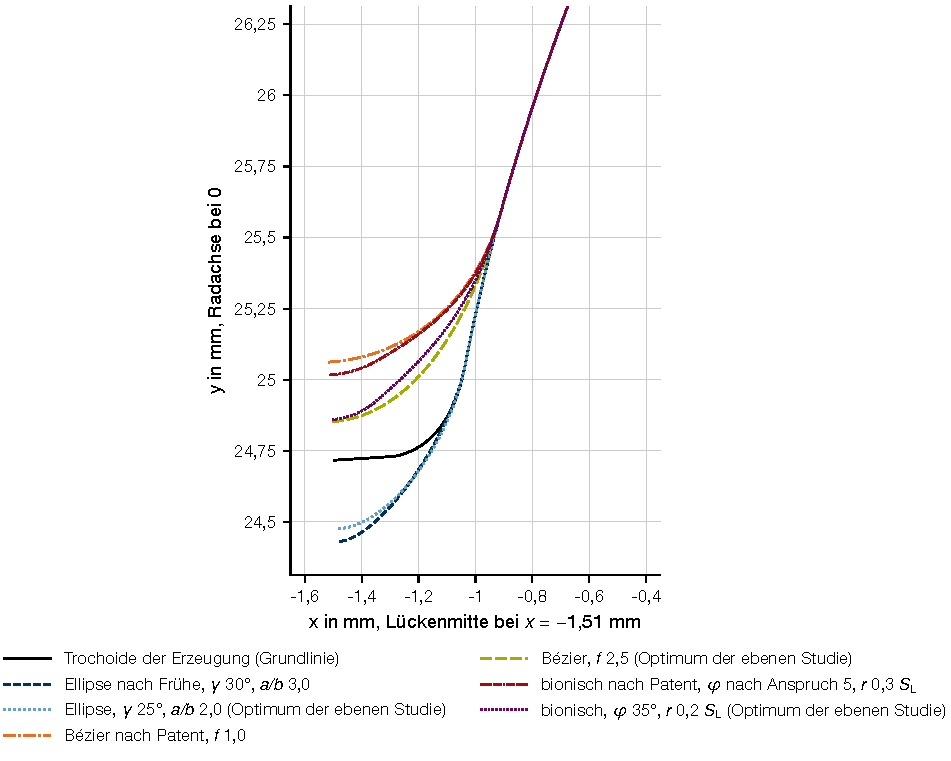
\includegraphics[width=0.85\textwidth]{kap3/fussrundungsvarianten}
    \caption{Fußrundungsvarianten des Rades kst-E im Stirnschnitt gegen die Trochoide der Erzeugung, linke Zahnhälfte von der Lückenmitte bis zur Evolvente. Die Ellipsen setzen am Fußformkreis an, die Patentkonturen am maßgebenden Durchmesser $d_{\mathrm{r}}$.}
    \label{fig:fussrundungsvarianten}
\end{figure}

Die Programme der Geometriekette, die Abaqus-Eingabedateien, die Datenauswertung und der Bildbau wurden in Python mit KI-gestützter Programmierung erstellt (Claude Code, Modell Fable 5.1). Zu jeder Rechenfunktion ist die Gleichung ihrer Quelle mit Ausgabe und Fundstelle vermerkt. Gerechnet wird durchgehend in doppelter Genauigkeit ohne Rundung innerhalb der Kette. Als pydantic-Modelle mit Prüfregeln sind die Datenstrukturen der Kette beschrieben, etwa für Wertebereiche und für die Reihenfolge der Durchmesser $d_{\mathrm{b}} \le d_{\mathrm{Ff}} < d_{\mathrm{Fa}} \le d_{\mathrm{a}}$. Eine fehlende Angabe wird gemeldet statt vorbelegt. Diese Beschreibung der Daten leitet zum Ausblick über, in dem Datenverträge für die Messprotokolle und die Rohdaten des Labors vorgeschlagen werden (\secref{sec:ausblick}).

% Bildwunsch: Konturvergleich gearcore gegen STplus (Zahnkontur-Export) / Konturen der drei Fußrundungsvarianten gegen die Trochoide
% (Labels im Text: fig:konturvergleich_stplus, fig:fussrundungsvarianten; noch nicht in bilder.yaml).

% Herkunft:
% Absatz 1 (Zweck, Normen): architecture_decisions.md ADR-105 Z. 137 bis 150 (aktuelle Norm gilt, DIN 3960
%   zurückgezogen, Abweichungen mit beiden Gleichungen und Zahlenbeispiel); norm_map.md Z. 8 bis 23 (Zuordnung
%   DIN 3960 → DIN ISO 21771, DIN 21773, DIN ISO 1328-1; DIN 867, DIN 3972).
% Absatz 2 (Erzeugung, Kontur): ADR-110 Z. 386 bis 393 (zwei von a_w, x_1, x_2; Kopfkreis ist Eingabe); ADR-111
%   Z. 517 bis 522 (Null wird angegeben); ADR-113 Z. 597 bis 620 (x_Es, Gl. (128) NB, Gl. (135), Schnittpunkt
%   numerisch, Hüllbedingung nach Linke und FVA 604 I, Ellipse der Kopfrundung) und Z. 621 bis 629 (Kantenbruch nach
%   DIN 3960 A.3.1 oder h_K und s_aK); contour.py Modul-Docstring Z. 1 bis 17 (Aufbau des Zahnes); norm_map.md
%   Z. 35 bis 37 (keine Norm gibt die Trochoide geschlossen an).
% Absatz 3 (Abgleich mit STplus): ADR-102 Z. 54 bis 66, Z. 85 bis 90 und Z. 97 (Stapelbetrieb, Konturexport,
%   Schnittstellendatei); ADR-106 Z. 165 bis 181 (einfache Genauigkeit, Toleranzen des Vergleichs); ADR-110
%   Z. 455 bis 457 (18 Fälle, 855 Vergleiche: 786 / 69 / 0); ADR-113 Z. 650 bis 651 und Z. 663 bis 665
%   (533 Vergleiche: 364 / 169 / 0; Konturen 0,6 / 0,25 µm, 14 Läufe, 28 Räder, vier unterschnitten, β bis 30°);
%   ADR-114 Z. 683 bis 686 und Z. 698 bis 702 (70 Probeläufe, Importer wendet Vorbelegungen an und vermerkt sie).
% Absatz 4 (Prüfmaße): ADR-115 Z. 856 bis 863 (DIN 21773, DIN 3977, STplus liest Prüfmaß als oberes Abmaß), Z. 867 bis
%   870 (Art des Maßes), Z. 876 bis 878 (Grenzmaße nach §4 mit x_Es, x_Em, x_Ei), Z. 879 bis 884 (k nach Gl. (9);
%   D_M aus DIN 3977 Tabelle 1 über Gl. (26), (27)), Z. 885 bis 896 (Regeln von STplus durch Bisektion der
%   Umschaltpunkte gefunden, 540 Zufallsräder, benannt, nie stillschweigend).
% Absatz 5 (Fußrundungsvarianten): ADR-116 Punkt 52 Z. 1793 bis 1822 (Konturersatz zwischen Übergang und Lückenmitte,
%   Ellipse nach Frühe Abschnitt 5.4.1 mit γ und a/b, Bézier nach DE 10 2013 004 861 B3 Anspruch 8 mit
%   k = (0,25 + 0,1 f) l und Bernstein-Form nach Roth und Opferkuch, bionisch nach DE 10 2008 045 318 B3 mit Tangens-
%   funktion, Kreis r, φ nach Anspruch 5, Übergang bei d_Ff bzw. d_r = (d_N + d_FR)/2, kinematische Prüfung, 0,02 mm,
%   Netzvorlage unverändert), Z. 1835 bis 1837 (Kassem 2023 bleibt außen vor), Z. 1846 bis 1851 (ebene Studie: drei
%   Zähne, eigener Löser, W1 16 Nm, Lastfleck an B, 42 / 7 / 36 Varianten); fillet.py Modul-Docstring Z. 1 bis 25,
%   Z. 235 bis 238 (l als Abstand des Hauptpunkts vom Tangentenschnittpunkt), Z. 340 bis 341 (d_FR als tiefster
%   Durchmesser, den der Gegenradkopf erreicht).
% Absatz 6 (Umsetzung): 00_schreibregeln.md Abschnitt 2 Punkt 3 (Nennung der KI-gestützten Programmierung, pydantic,
%   Ausblick); gearcore README.md Z. 3 und Z. 13 bis 14 (pydantic-Datenverträge, jede Rechenfunktion nennt Quelle und
%   Gleichung); ADR-106 Z. 171 bis 175 (doppelte Genauigkeit ohne Rundung in der Kette); ADR-110 Z. 413 bis 422
%   (Prüfregeln: Typen, Wertebereiche, d_b ≤ d_Ff < d_Fa ≤ d_a); norm_map.md Z. 297 bis 300 (fehlender Wert wird
%   gemeldet, keine stillen Vorbelegungen).
% Zitate: ISO14 = DIN ISO 21771 (2014), DIN14 = DIN 21773 (2014), DIN86 = DIN 867 (1986), Lin10 = Linke 2010,
%   Frue12 = Frühe 2012 (Schlüssel in der Bib: Frü12). Rot17 ist FVA 732 I (Roth Z.), nicht Roth und Opferkuch 2017
%   (VDI-Berichte 2294): deshalb Platzhalter. Keine Bib-Einträge für DIN 3972, FVA 604 I, STplus-Programmanleitung,
%   die beiden Patente und Kassem 2023 (Zim16 ist FVA 604 II).


\section{Simulationskette und FE-Modell}
\label{sec:fe_modell}
% Entwurf 2026-10-17 (T1). Zitierschlüssel: Stommel et al. 2018 liegt in der .bib unter Sto18
% (Sto18 ist Stoffregen, Motorradtechnik); DIN ISO 21771:2014 unter ISO14.

Die Beanspruchung des Kunststoffrades wird mit einem Finite-Elemente-Modell der Paarung aus Stahlritzel und Kunststoffrad berechnet. Dieser Abschnitt beschreibt die Programme, aus denen die Eingaben stammen, den Aufbau des Modells, die Werkstoffstufen mit ihren Dehnraten und den Umfang der Rechnungen. Die Auswertung folgt in \secref{sec:auswertung_beanspruchung}, die Ergebnisse stehen in \chapref{chap:voruntersuchungen} und \chapref{chap:berechnung}.

% TK erledigt (alle Verweise über die fetten Makros, rohe \ref ersetzt): Kapitelverweise hatten wir doch auch dick oder?

\subsection{Simulationskette}
\label{sec:simulationskette}

Die Werkstoffdaten des Rades durchlaufen vor der FE-Rechnung mehrere Programme. Aus Zugversuchen passt Matscape die Werkstoffkarten an, CADMOULD berechnet die Faserorientierung des spritzgegossenen Rades, CONVERSE überträgt sie auf das FE-Netz, und ein eigenes Programm in Python schreibt daraus die Eingabedateien für Abaqus/Standard.
\figref{fig:flussbild_kette} zeigt die Kette mit den Programmen und den Daten, die zwischen ihnen übergeben werden.

\begin{figure}[htbp]
	\centering
	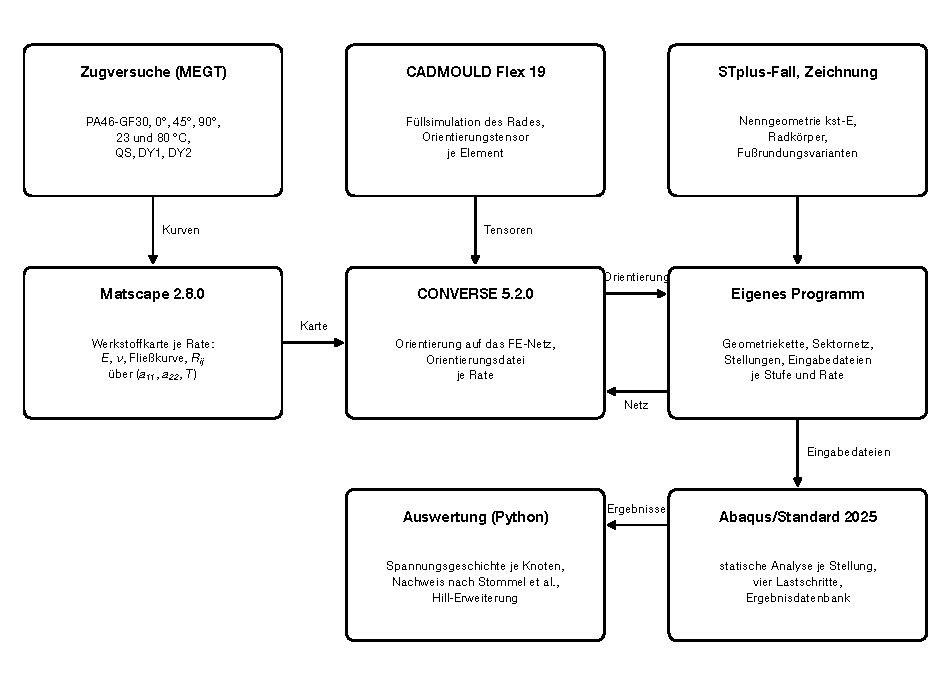
\includegraphics[width=0.95\textwidth]{kap3/flussbild_kette}
	\caption{Simulationskette von den Zugversuchen zum Nachweis: Programme als Kästen, die übergebenen Daten an den Pfeilen.}
	\label{fig:flussbild_kette}
\end{figure}

Die Zugversuche wurden am Lehrstuhl für Maschinenelemente, Getriebe und Tribologie (MEGT) der Rheinland-Pfälzischen Technischen Universität Kaiserslautern-Landau durchgeführt. Werkstoff war das konditionierte PA46-GF30 Stanyl TW200F6 von Envalior, geprüft bei $23$ und $80$\,\textdegree C an Proben unter $0$\textdegree, $45$\textdegree{} und $90$\textdegree{} und bei drei Prüfgeschwindigkeiten. Der quasistatischen Karte QS liegen die Richtungen $0$\textdegree{} und $90$\textdegree{} zugrunde, den dynamischen Karten DY1 und DY2 alle drei Richtungen. Matscape 2.8.0 von PART Engineering passt an diese Kurven je Prüfgeschwindigkeit eine Werkstoffkarte an. Sie enthält die elastischen Konstanten als Gitter über dem Orientierungszustand und der Temperatur. Der Zustand wird durch die beiden größten Eigenwerte $a_{11}$ und $a_{22}$ des Orientierungstensors beschrieben. Dazu kommen die Fließkurve des $0$\textdegree-Stabes als wahre Spannung und die Fließspannungsverhältnisse nach Hill je Orientierungszustand. Die Versagensart stuft Matscape aus den Versuchsdaten als duktil ein.

Die Faserorientierung stammt aus einer Spritzgießsimulation des Rades mit Cadmould Flex 19.0.1.10 in der Strategie 3D-F mit einer Elementkante von $1$\,mm. Das reale Werkzeug mit dem Stahleinleger und dem später abgetrennten Zentralanguss stand nicht zur Verfügung. Ein virtueller Verteiler mit 238 Anspritzpunkten auf den Radien $15{,}0$ bis $19{,}1$\,mm in der Stegebene füllt deshalb das Bauteil. \tabref{tab:cadmould} nennt die Prozessparameter des Laufs. Das Orientierungsergebnis liegt als binäre Datei vor, die hier nicht gelesen wird. In die Kette geht es allein über CONVERSE ein.

\begin{table}[htbp]
	\caption{Einstellungen der Spritzgießsimulation des Rades in CADMOULD.}
	\label{tab:cadmould}
	\centering
	\small
	\begin{tabular}{ll}
		\hline
		Größe                            & Wert                                                                       \\
		\hline
		\arrayrulecolor{black!30}
		Programm und Strategie           & Cadmould Flex 19.0.1.10, 3D-F                                              \\
		\hline
		Elementkante in mm               & $1$                                                                        \\
		\hline
		Werkstoff                        & Stanyl TW200F6 (Envalior)                                                  \\
		\hline
		Faserfaktoren                    & $0{,}99$; $0{,}94$; $0{,}09$                                               \\
		\hline
		Interaktionskoeffizient          & $0{,}01$                                                                   \\
		\hline
		Anspritzung                      & virtueller Verteiler, 238 Punkte, $r$ $15{,}0$ bis $19{,}1$\,mm, Stegebene \\
		\hline
		Füllzeit in s                    & $0{,}554$                                                                  \\
		\hline
		Massetemperatur in \textdegree C & $315$                                                                      \\
		\hline
		Wandtemperatur in \textdegree C  & $100$                                                                      \\
		\hline
		Nachdruck in bar, Dauer in s     & $500$; $10{,}9$                                                            \\
		\arrayrulecolor{black}
		\hline
	\end{tabular}
\end{table}

CONVERSE 5.2.0 überträgt das Orientierungsergebnis auf das Netz des FE-Modells. Die Ausgabe ist eine Orientierungsdatei im Abaqus-Format. Sie enthält je Element das Faserkoordinatensystem als Verteilung, je Knoten die Eigenwerte $a_{11}$ und $a_{22}$ als Feldvariablen und die Werkstoffkarte der Rate. Für jede Rate entsteht eine Datei. Die Orientierungszeilen der drei Dateien sind gleich, nur die Werkstofftabellen unterscheiden sich. Da die Elementnummern jedes Netzes eigen sind, braucht jeder Körper und jede Fußrundungsvariante ein eigenes CONVERSE-Mapping. Vor dem Schreiben der Eingabedateien wird geprüft, dass Element- und Knotennummern der Orientierungsdatei genau die des Netzes sind und der Name der Karte zur Rate passt. Der Sektor liegt in jedem CONVERSE-Mapping an derselben Winkelstellung des Rades, weil das Spritzgießergebnis nicht rotationssymmetrisch ist (vgl. \secref{sec:faserorientierung}).

Netz und Eingabedateien erzeugt das in \secref{sec:werkzeugkette} beschriebene Programm. Es baut den Sektor aus der erzeugten Zahnkontur und dem Radkörper der Zeichnung und schreibt je Stellung, Werkstoffstufe und Rate eine Eingabedatei. Die Orientierungsdatei wird dafür in einen Teil für das Bauteil und einen Teil für das Modell zerlegt. Der Elementsatz ihrer Querschnittsdefinition wird auf den des Netzes umgeschrieben. Eine Manifestdatei je Ordner hält Netz, Stellungen, Momente, Karten und Lösereinstellungen fest (vgl. \anhref{sec:anhang_c}).

Gerechnet wird mit Abaqus/Standard 2025 auf einer Vollversion mit vier Kernen. Funktionstests kleiner Modelle liefen in der Learning Edition. Die Ergebnisdatenbanken werden nach \secref{sec:auswertung_beanspruchung} ausgelesen und bleiben erhalten, so dass weitere Größen nachträglich gelesen werden können.

Neben Abaqus dient ein eigener ebener Löser der Konvergenzstudie und der ebenen Fußrundungsstudie (\secref{sec:netzkonvergenz}, \secref{sec:werkzeugkette}). Er rechnet den Stirnschnitt des Sektors im ebenen Dehnungszustand linear elastisch, isotrop und mit kleinen Verschiebungen. Das Vierknotenelement liegt in zwei Formulierungen vor, selektiv reduziert integriert wie CPE4 und C3D8 sowie mit inkompatiblen Moden wie CPE4I und C3D8I. Die Spannungen werden wie in Abaqus von den Gaußpunkten auf die Knoten extrapoliert und gemittelt. Am Einzahnsektor mit 859 Knoten stimmt er mit Abaqus in der Learning Edition auf $7 \cdot 10^{-5}$ überein.

Die Paarung wird ausschließlich in Abaqus gerechnet. Ein eigenes Modell wurde aufgebaut, weil die FVA-Workbench als geschlossenes Werkzeug Konvergenzstudien über mehrere Netze nur bedingt zulässt. Zudem sollte die vollständige Kette skriptbasiert in Python umgesetzt werden, um diese Art der Programmierung zu erlernen. Nachträglich geänderte Eingabedateien der Workbench konvergierten bei werkstofflicher und geometrischer Nichtlinearität außerdem schlecht. Das Netz der Verzahnung kst-E, mit dem die Zahnfußspannung dort ausreichend aufgelöst ist, dient als Ausgangsdiskretisierung.

\subsection{Aufbau des Modells}
\label{sec:fe_modellaufbau}

Das Rad wird als Sektor aus fünf Zähnen mit je einem zahnlosen Teilungsabschnitt an beiden Enden modelliert. Die Topologie des Stirnschnitts stammt von einem Referenzmodell der FVA Workbench zur Verzahnung kst-E \cite{FVA856-I}, dessen Schnitt entlang der Lückenmitten in einen Schulterblock und kongruente Zahnblöcke zerfällt. Auf die erzeugte Kontur werden die Oberflächenknoten stückweise gesetzt, so dass Fußformpunkt, Kopfformpunkt und Kopfecke Knoten sind. Das Innere folgt durch harmonische Fortsetzung der Oberflächenverschiebung. \figref{fig:netz_sektor} zeigt den Sektor, \figref{fig:netz_zahn} den Stirnschnitt eines Zahns mit der Randschicht an Flanke und Fußrundung.

% TK erledigt (Grid über plot_style axes.axisbelow in allen Bildern nach hinten): Hier in dem Bild fällt es richtig auf, dass das Grid über den eigentlich zu sehenden Bild ist. Das Grid soll aber immer in der hintersten Ebene liegen, dass es das geezigt nicht überlappt. Bitte auch nochmal bei anderen Bildern überprüfen. Bild 3.5 ist beispielsweise korrekt.

\begin{figure}[htbp]
	\centering
	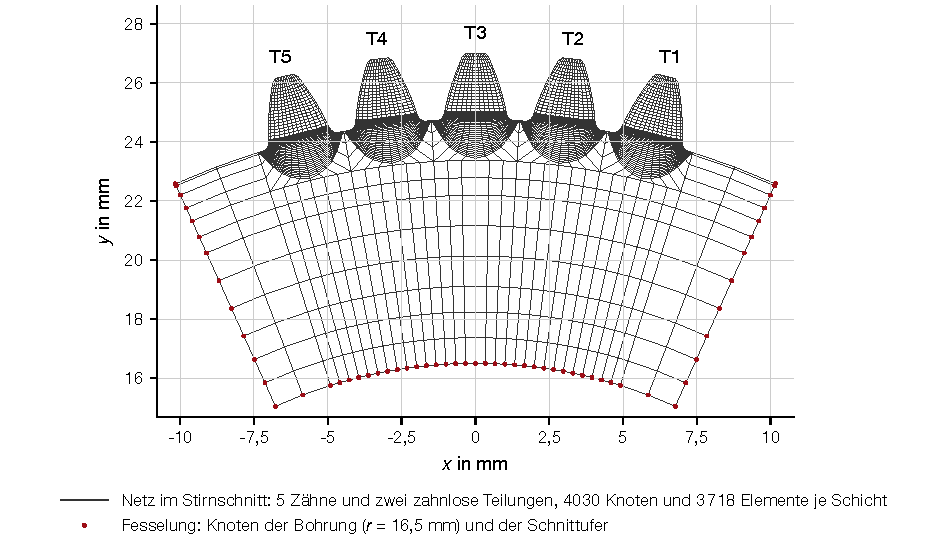
\includegraphics[width=0.7\textwidth]{kap3/netz_sektor}
	\caption{Sektornetz des Rades mit Taschenkörper, 20 Schichten über der Zahnbreite, Bohrung $33$\,mm.}
	\label{fig:netz_sektor}
\end{figure}

\begin{figure}[htbp]
	\centering
	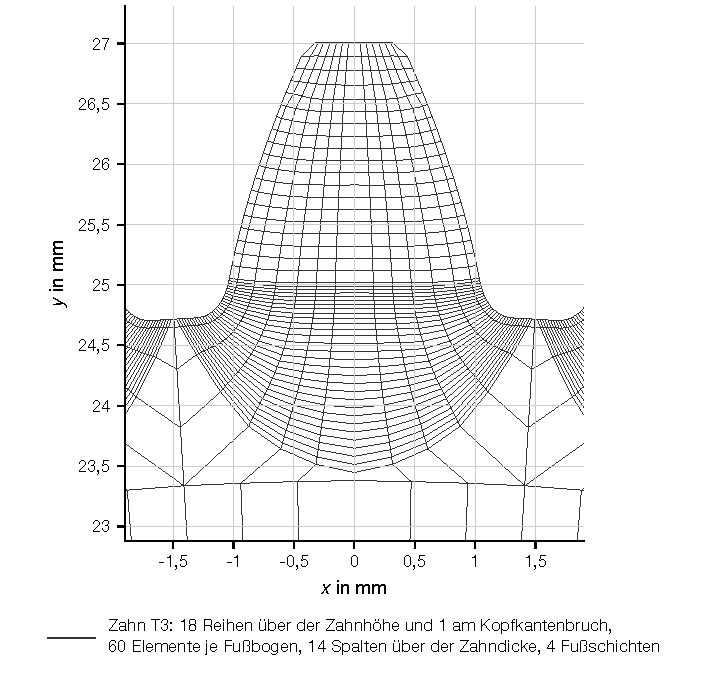
\includegraphics[width=0.7\textwidth]{kap3/netz_zahn}
	\caption{Netz eines Zahns im Stirnschnitt: Randschicht an Flanke und Fußrundung, Vergröberung zum Körper.}
	\label{fig:netz_zahn}
\end{figure}

Die Diskretisierung folgt der Konvergenzstudie am ebenen Sektor in \secref{sec:netzkonvergenz}. Sie ist je Bereich des Zahns verschieden fein. Über der Zahnhöhe liegen 18 Elementreihen und eine am Kopfkantenbruch, am Fußbogen 60 je Lücke, über der Zahndicke 14, dazu vier Fußschichten normal zur Fußoberfläche und zwei Spalten je Schulter. In Richtung der Zahnbreite von $15$\,mm liegen 20 Schichten. Dieses Netz ist die Grundlage jedes CONVERSE-Mappings der Faserorientierung.

Der Radkörper folgt der überbemaßten Zeichnung des Rades (vgl. \anhref{sec:anhang_a}). Die Nabe reicht in voller Breite von der Bohrung mit dem Radius $16{,}5$\,mm bis zum Radius $19{,}107$\,mm. Von beiden Stirnseiten ist je eine Tasche bis zum Radius $22{,}168$\,mm eingeformt, $5{,}5$\,mm tief, mit Wänden unter $93$\textdegree{} zur Stirnseite. Zwischen den Taschen bleibt ein Steg von $4$\,mm, vergleichbar mit einem I-Profil in voller Breite der Zähne. Die Rundungen R\,$0{,}5$ der Zeichnung sind nicht vernetzt. Das Stirnschnittnetz behält seine Zahnzone. Die Ringe des I-Profils werden Schicht für Schicht auf Bohrung, Nabenwand und Profilwand gelegt, wobei die Formschräge der Wände mitgeht. Die Elemente innerhalb der Taschen werden entfernt. Das I-Profil erhält acht Ringe, der Steg sechs Schichten und jede Tasche sieben. Der Taschenkörper hat damit 83\,650 Knoten und 72\,932 Elemente (vgl. \figref{fig:netz_koerper}). Der Vollring mit Bohrung, der Bezugskörper der Netzstudien in \chapref{chap:voruntersuchungen}, wird dort auf derselben Schichtung wie der Taschenkörper geführt und hat 82\,425 Knoten und 72\,320 Elemente. Er trägt trotz des vollen Querschnitts weniger Elemente, weil er radial nur fünf Kranzringe hat.

% TK erledigt (Zahlen des Rings auf Taschenschichtung, Grund: fünf gegen acht Ringe): Warum hat der Vollring weniger Elemente und Knoten als der Taschenkörper. Das hatten wir doch geklärt, dass wir den Vollring dann nur noch mit dem angepassten mesh vom I-Profilkörper verwednen. Bitte von dem die Werte dort im Text einsetzen.

\begin{figure}[htbp]
	\centering
	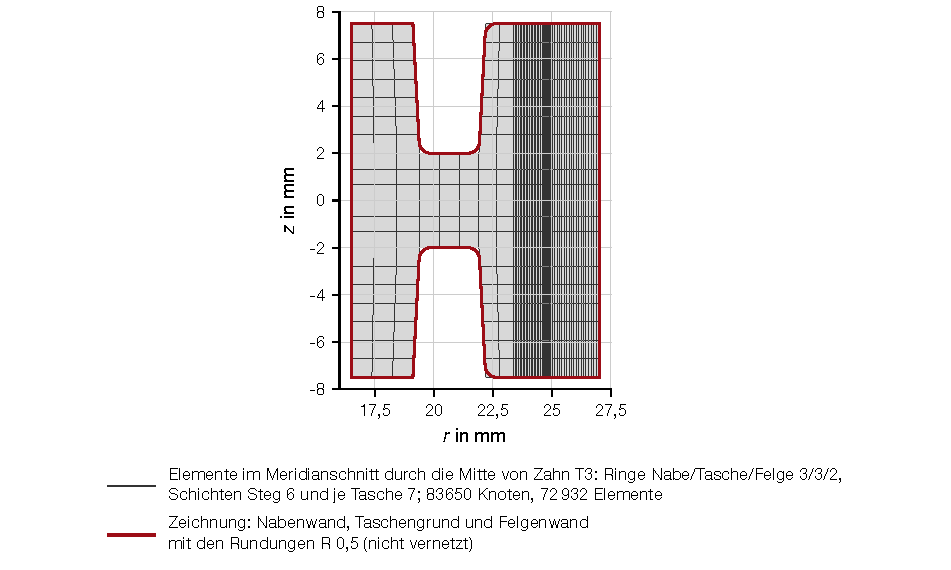
\includegraphics[width=0.7\textwidth]{kap3/netz_koerper}
	\caption{Radkörper nach Zeichnung: Nabe, Steg und Taschen mit Formschräge.}
	\label{fig:netz_koerper}
\end{figure}

% TK erledigt (Bild in 3.1 gestrichen, hier mit z horizontal neu): Das Bild gibt es schonmal. Hier deutlich aufgeräumter. Die ganzen Bezeichnungen an der anderen Stelle braucht es nicht. Bitte nur hier einbinden und nicht an der ersten Stelle. DAs reicht. Dennoch wie in der anderen Markierung genannt die z-Achse auf die Horizontale legen, dass kann ess sich der LEser besser Vorstellen und verstehte die Bezeichnung I-Profil über den Umfang.

Der Stahleinleger des realen Rades sitzt in der Bohrung mit $33$\,mm Durchmesser. Er wird nicht vernetzt, sondern als starre Fesselung abgebildet. Bohrungsknoten und beide Schnittflächen des Sektors sind als starrer Körper an den Bezugspunkt des Rades gebunden, der in allen Freiheitsgraden festgehalten ist. Weil die festen Schnittflächen auf die äußeren Zähne zurückwirken, wird der mittlere Zahn T3 ausgewertet.

Das Stahlritzel geht nur mit seiner Zahnoberfläche in das Modell ein, als starre Fläche aus vierknotigen Elementen R3D4 mit Facetten bis $0{,}05$\,mm Kantenlänge, ohne Volumen, Stirnflächen und Werkstoff. Sie umfasst sieben Zähne und ist an einen Bezugspunkt auf der Ritzelachse gebunden, der Drehung und Moment aufnimmt. Dass das Ritzel als starre Fläche modelliert wird, folgt aus der Paarung Stahl gegen Kunststoff. Die Kopfkanten des Ritzels sind in dieser Fläche gerundet, mit $0{,}1$\,mm und zwölf Facetten je Bogen. Das reale Ritzel hat nach Zeichnung und Konturscan eine scharfe Kante. Die Rundung ist eine Entscheidung des Modells, die in \secref{sec:kopfkante} aus den Abbrüchen an der scharfen Kante begründet und in ihrem Einfluss untersucht wird. \figref{fig:paarung_netz} zeigt Sektor und Ritzelfläche in der Rechenlage im Normpunkt C.

\begin{figure}[htbp]
	\centering
	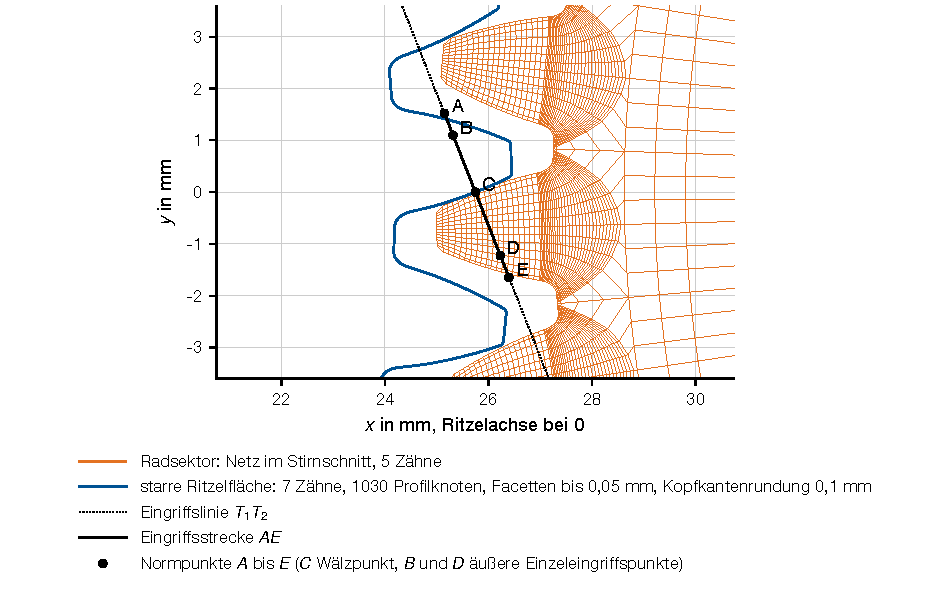
\includegraphics[width=0.7\textwidth]{kap3/paarung_netz}
	\caption{Radsektor und starre Ritzelfläche in der Stellung C mit Eingriffslinie und den Normpunkten A bis E.}
	\label{fig:paarung_netz}
\end{figure}

% TK erledigt (Grid nach hinten): Auch hier das Grid in der vordersten und nicht hintersten Ebene. Wie, wenn man auf einem Karierten Papier schreibt musst du dir vorstellen. Da überdeckt die Tinte auch den Blatthintergrund. Deswgen Grid nach hinten.

Die Lage des Paares wird je Stellung analytisch aus der Evolventengeometrie bestimmt. Eine einzige Größe, der Krümmungsradius der Ritzelflanke im Berührpunkt des verfolgten Zahnpaares, legt beide Räder fest. Die Arbeitsflanken berühren sich, das gesamte Flankenspiel liegt an den Rückflanken. Der Drehsinn ist der des Prüfstands. Bei Blick auf die Stirnseite mit dem Ritzel links dreht das treibende Ritzel im Uhrzeigersinn, und die rechten Flanken arbeiten. Beide Räder sind als Bauteile mit festen Achsen definiert und werden je Stellung als Instanzen verschoben und um ihre Achsen gedreht. Eine am Bauteil definierte Orientierung dreht in Abaqus mit der Instanz mit, auch wenn sie als Verteilung vorliegt, so dass die Faserorientierung dem Rad in jede Stellung folgt. Bei jedem Lauf mit Orientierungsdatei wird dies an den lokalen Werkstoffrichtungen der Ergebnisdatenbank geprüft.

Der Kontakt ist als Knoten-zu-Fläche-Paar mit der Radflanke als Nebenfläche und der starren Ritzelfläche als Hauptfläche definiert. Die Normalen der facettierten starren Fläche werden mit dem Glättungsmaß $0{,}2$ geglättet, so dass die Kontaktkraft normal zur Ritzelflanke bleibt. Die Kontaktbedingung ist hart und reibungsfrei und wird mit Lagrange-Multiplikatoren erzwungen, der Voreinstellung von Abaqus für diese Formulierung. Stabilisierung, Dämpfung und Masse sind ausgeschlossen. Die Lösereinstellungen und Iterationsgrenzen stehen in \anhref{sec:anhang_c}. Die Wahl der Kontaktformulierung wird in \secref{sec:kopfkante} begründet.

% TK erledigt (Pilotergebnisse zu Iterationsgrenzen und Fläche-zu-Fläche gestrichen; ebenso gestrichen: 40/80-Schichten-Piloten im Netzabsatz, NLGEOM-Prozente und C3D8I-Abbrüche im Stufenabsatz, alle mit Verweis auf 4.1): Der Abschnitt greift schon zu sehr dem Kapitel 4 vor, wo die Netzkonvergenz durchprobiert wurde. Bitte rausnehmen. Ich mache es bewusst nicht manuell, dass du den Fehler merkst und auch bei anderen Abschnitten Kürzungen vorschlägst, die thematisch einem anderen Kapitel/Abschnitt gehören.

Jede Rechnung ist eine implizite statische Analyse mit vier Schritten. Im ersten Schritt wird dem Ritzel eine Drehung um einen Bogen von $1$\,\textmu m am Grundkreis vorgegeben, die den Kontakt schließt. Danach folgen drei statische Schritte, in denen die Vorgabe entfällt und das Moment als Last auf den Drehfreiheitsgrad des Ritzels wirkt. Die Momente am Rad betragen $8$, $12$ und $16$\,Nm wie im Laufversuch und werden am Ritzel mit
\begin{equation}
	T_1 = T_2 \, \frac{z_1}{z_2}
	\label{eq:moment_ritzel}
\end{equation}
aufgebracht, dem Betrag nach $7846$, $11\,769$ und $15\,692$\,Nmm. Das Vorzeichen folgt dem Drehsinn des Prüfstands, so dass das treibende Ritzel die Arbeitsflanke des Rades belastet. Das Ritzel dreht sich unter dem Moment bis zum Gleichgewicht. Nichts wälzt innerhalb einer Analyse ab. Dieser Verdrehwinkel des Ritzels bis zum Gleichgewicht ist in den folgenden Kapiteln das Maß der Verformung. Er enthält die Biegung der Radzähne und die Nachgiebigkeit des Kontakts, nicht das Flankenspiel, weil die Arbeitsflanken zu Beginn jeder Rechnung berühren. Je Schritt werden Spannungen, Dehnungen, Verschiebungen und Kontaktgrößen in die Ergebnisdatenbank geschrieben, dazu Kräfte, Stützmoment und Drehung beider Bezugspunkte in die Textausgabe.

% TK erledigt (Moment als Betrag mit Drehsinn des Prüfstands; Verdrehwinkel definiert): Drehsinn mit im Uhrzeigersinn vom Text und x y aus den Bildern würde bei der Angabe eines positiven Moment gegen Uhrzeigersinn nach rechter Hand und Daumenregel drehen. Bitte entweder Betrag einbinden oder anders formulieren.

Die Eingriffsstrecke wird nicht in einer Abwälzsimulation durchlaufen, sondern in Einzelstellungen. Nach Stommel et al. \cite[S.~56 bis 57]{Sto18} sind elastisch-plastische Werkstoffmodelle für Kunststoffe nur unter monotoner Belastung sinnvoll. Ein an der Spannungs-Dehnungs-Kurve kalibriertes Modell zählt viskoelastische Dehnung als plastische und weist die bleibende Dehnung zu groß aus. Ein Abwälzen be- und entlastet jeden Zahn, und die Lastgeschichte, die es mitführen würde, bestünde aus genau diesen Dehnungen. Die Erstbelastung je Stellung ist die Belastung, für die das Modell gilt. Für elastischen Werkstoff führen beide Wege zum gleichen Zustand, so dass das Abwälzen in einer Simulation als Gegenprobe mit elastischem Werkstoff dem Ausblick vorbehalten bleibt (vgl. \secref{sec:ausblick}).

% TK erledigt (S. 56 bis 57; alle Zitate ohne Seite werden in Paket A3 nachgezogen): Zitat nur noch ohne Seite. Entweder in der gesamten Arbeit mit Seitenzahlen beim zitieren arbeiten oder gar nicht. Bitte einheitlich. Gerne mit Seitenzahlen.

Die Stellungen liegen auf einem Gitter über dem Eingriffsweg mit 30 Stellungen je Eingriffsteilung, von einer Teilung vor dem Eingriffsbeginn A bis eine Teilung nach dem Eingriffsende E. Zusätzlich werden die Normpunkte A bis E als eigene Stellungen gerechnet. Die äußeren Einzeleingriffspunkte B und D folgen DIN ISO 21771 \cite{DINISO21771}. Mit $p_{\mathrm{bt}} = 2{,}952$\,mm und $g_{\alpha} = 3{,}406$\,mm ergibt das 99 Stellungen je Serie. Der Rand von einer Teilung deckt den durch die Verformung verlängerten Eingriff ab. Gitterweite und Rand wurden in den Voruntersuchungen festgelegt (vgl. \chapref{chap:voruntersuchungen}). Die Lage des Paares in der Stellung C mit der Eingriffsstrecke zeigt \figref{fig:paarung_netz}.

\subsection{Werkstoffstufen und Dehnraten}
\label{sec:werkstoffstufen}

Der Werkstoff des Rades wird in vier Stufen beschrieben, die alle auf derselben Karte beruhen und außerhalb der Werkstoff- und Querschnittsblöcke gleiche Eingabedateien haben (vgl. \tabref{tab:werkstoffstufen}). W1 nimmt die isotrope Zeile der Karte bei $80$\,\textdegree C als linear elastischen Werkstoff. W2 ergänzt sie um die Fließkurve und die Fließspannungsverhältnisse nach Hill derselben Zeile. Da Abaqus anisotrope Fließbedingungen nur in einem lokalen System zulässt, trägt W2 das Bauteilsystem als Orientierung. W3 verwendet die Orientierungsdatei ohne Plastizität, die elastischen Konstanten folgen dann je Element dem Orientierungszustand des CONVERSE-Mappings. W4 verwendet die vollständige Orientierungsdatei.

Elementtyp und Kinematik richten sich nach der Stufe. Die elastischen Stufen W1 und W3 werden geometrisch linear mit C3D8I, dem Element mit inkompatiblen Moden, gerechnet. Die elastisch-plastischen Stufen W2 und W4 werden geometrisch nichtlinear mit C3D8, dem Element mit selektiv reduzierter Integration, auf demselben Netz gerechnet. Die nichtlineare Rechnung ist gewählt, weil die Fließkurve der Karte bei $80$\,\textdegree C schon bei $4{,}3$\,MPa beginnt und Stommel et al. für Kontakt und große Verformung den nichtlinearen Löser vorsehen \cite[S.~474]{Sto18}. Die Gründe für diese Zuordnung, die Abbrüche von C3D8I unter geometrischer Nichtlinearität und das Konvergenzverhalten beider Elemente stehen in \secref{sec:netzkonvergenz}. Fußspannungen werden nur innerhalb eines Elementtyps verglichen.

\begin{table}[htbp]
	\caption{Werkstoffstufen des FE-Modells, Datenquelle, Elementtyp und Kinematik.}
	\label{tab:werkstoffstufen}
	\centering
	\small
	\begin{tabular}{lL{4.2cm}L{4.8cm}ll}
		\hline
		Stufe & Werkstoffmodell                & Datenquelle                         & Element & NLGEOM \\
		\hline
		\arrayrulecolor{black!30}
		W1    & isotrop, linear elastisch      & isotrope Zeile der Karte            & C3D8I   & nein   \\
		\hline
		W2    & isotrop, elastisch-plastisch   & isotrope Zeile, Fließkurve, Hill    & C3D8    & ja     \\
		\hline
		W3    & anisotrop, elastisch           & Orientierungsdatei ohne Plastizität & C3D8I   & nein   \\
		\hline
		W4    & anisotrop, elastisch-plastisch & vollständige Orientierungsdatei     & C3D8    & ja     \\
		\arrayrulecolor{black}
		\hline
	\end{tabular}
\end{table}

Die drei Karten unterscheiden sich in der Prüfgeschwindigkeit der zugrunde liegenden Zugversuche (vgl. \tabref{tab:raten}). Die Steifigkeit wächst mit der Dehnrate. Jede Werkstoffstufe wird mit jeder Rate gerechnet. W1 und W2 nehmen die isotrope Zeile der Karte ihrer Rate, so dass die Ratenachse für alle vier Stufen gilt. Alle Karten werden bei $80$\,\textdegree C ausgewertet, weil die Laufversuche auf diese Zahnmassentemperatur geregelt sind (\secref{sec:pruefstand}, \secref{sec:temperatur}).

In \figref{fig:orientierungszustaende_qs} stehen die gemessenen Kurven in und quer zur Fließrichtung neben den Kurven dreier Orientierungszustände der quasistatischen Karte. Jede Zustandskurve entsteht aus der Referenzkurve in Fließrichtung durch Skalieren mit dem Fließspannungsverhältnis und dem Modul des Zustands. Der Zustand des Zahnfußes ist der Orientierungszustand, den das CONVERSE-Mapping am Fuß des Zahns T3 liefert, mit den Eigenwerten $a_{11} = 0{,}64$ und $a_{22} = 0{,}083$. Die Orientierungsdateien tragen je Element diesen Tensor, die Karte das Kennwertgitter, aus dem die Kurve des Zustands interpoliert wird. Der isotrope Zustand liegt nahe der Messung quer zur Fließrichtung. Das erklärt sich daraus, dass ein regellos orientierter Kurzfaserverbund in jeder Richtung nur einen kleinen Teil der Faserwirkung trägt. Die Probe quer zur Fließrichtung aus einem hochorientierten Stab besitzt dagegen noch Restverstärkung. Der ausgerichtete Zustand liegt deutlich über der Messung in Fließrichtung, und der stark ausgerichtete Fußzustand trifft annähernd die Messung in Fließrichtung.

\begin{figure}[htbp]
	\centering
	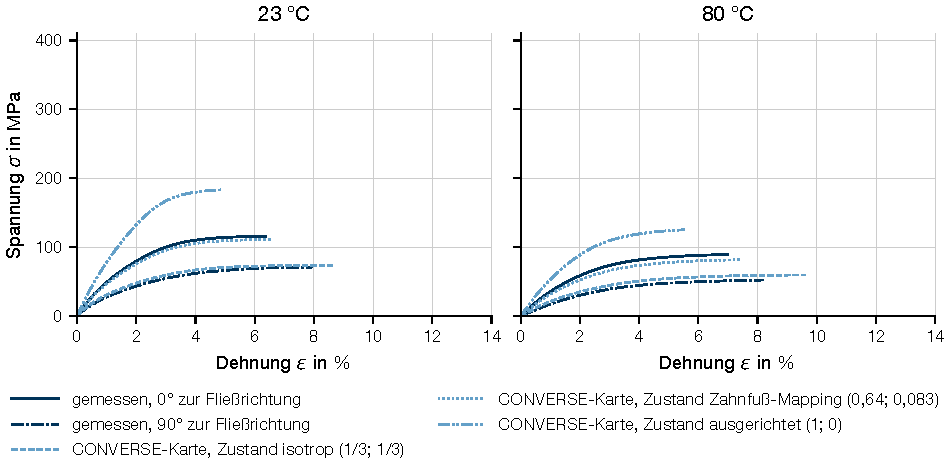
\includegraphics[width=0.95\textwidth]{kap2/orientierungszustaende_qs}
	\caption{Gemessene Richtungen und Orientierungszustände der quasistatischen Werkstoffkarte von PA46-GF30 bei $23$ und $80$\,\textdegree C (Matscape-Karte, Zustandskurven aus der Referenzkurve in Fließrichtung mit $R_{\mathrm{11}}$ und $E_{\mathrm{1}}$ des Zustands).}
	\label{fig:orientierungszustaende_qs}
\end{figure}

\begin{table}[htbp]
	\caption{Werkstoffkarten der drei Dehnraten. $E$ und $\nu$ aus der isotropen Zeile jeder Karte bei $80$\,\textdegree C.}
	\label{tab:raten}
	\centering
	\small
	\begin{tabular}{llllll}
		\hline
		Karte & Prüfgeschwindigkeit in m/s & Dehnrate in 1/s             & $E$ in MPa  & $\nu$      & Temperatur in \textdegree C \\
		\hline
		\arrayrulecolor{black!30}
		QS    & $0{,}0000167$              & $0{,}00027$ bis $0{,}00044$ & $2282{,}08$ & $0{,}2997$ & $80$                        \\
		\hline
		DY1   & $0{,}174$                  & $3$                         & $2542{,}51$ & $0{,}2951$ & $80$                        \\
		\hline
		DY2   & $10$                       & $60$                        & $3596{,}61$ & $0{,}2973$ & $80$                        \\
		\arrayrulecolor{black}
		\hline
	\end{tabular}
\end{table}

Welche Karte dem Prüfstand am nächsten kommt, folgt aus der Dehnungsgeschichte des Zahnfußes im Modell. Bei $3000$\,1/min am Rad läuft der Berührpunkt mit $7{,}7$\,m/s über die Eingriffslinie, eine Teilung in $0{,}385$\,ms, und die Zugspannung der Fußrundung steigt vom Eintritt des Zahns bis zu ihrem Größtwert über rund $3{,}2$\,mm Wälzweg, also in $0{,}42$\,ms, auf $2{,}6$ bis $3{,}8$\,\% Dehnung der Stufe W1. Das ergibt je Stufe einen Wert, $60$\,1/s bei $8$\,Nm und $90$\,1/s bei $16$\,Nm mit dem Modul der quasistatischen Karte und $45$ beziehungsweise $70$\,1/s mit dem Modul der Karte DY2, bei $2250$\,1/min jeweils drei Viertel davon (\secref{sec:stufen_raten_koerper}). Die Karte DY2 mit $60$\,1/s liegt dem Prüfstand damit am nächsten, QS ist die untere Grenze.

% TK erledigt (Nullen ergänzt, Ursache: latexindent 4.0 entfernt die 0 nach einem Dollarzeichen; Satz zur Karte der Belastungsgeschwindigkeit ergänzt): In der Tabelle werden die 0 en vor dem Komma angezeigt in anderern Tabellen und manchmal im Text nicht. Bitte die 0 vor dem Komma überall geränzen. Vielleicht noch einen Satz erwähnen, welche Karte der realen Belastungsgeschwindigkeit am nähsten kommt, wenn es nicht an anderer Stelle erwähnt wird.

Als zweite Werkstoffquelle der anisotropen elastischen Stufe dienen die elastischen Konstanten der konditionierten Randschicht aus Tabelle~4 des Abschlussberichts FVA 856 I \cite{FVA856-I} (vgl. \tabref{tab:fva856_tab4}). Der Bericht hat sie aus Zugversuchen an $0$\textdegree- und $90$\textdegree-Proben mit einer mikromechanischen Zelle umgerechnet. In dieser Variante ersetzt der Block mit den neun Konstanten bei $80$\,\textdegree C und der jeweiligen Rate den orientierungsabhängigen Elastizitätsblock der Karte. Die Konstanten gelten unverändert über dem ganzen Rad im Faserkoordinatensystem, das das CONVERSE-Mapping je Element vorgibt. Die Richtung 1 ist die Faservorzugsrichtung. Daneben wurde eine zweite Richtungsquelle aufgebaut, in der die Zonenkarte der CT-Befunde des Berichts den fünf Zähnen des Sektors zugewiesen wird. Werkstoffquelle und Richtungsquelle werden so in einem Schema aus zwei mal zwei Varianten getrennt (vgl. \secref{sec:faserorientierung}).

\begin{table}[htbp]
	\caption{Elastische Konstanten der konditionierten Randschicht von PA46-GF30 bei $80$\,\textdegree C nach Tabelle~4 des Berichts FVA 856 I. Richtung 1 Faservorzugsrichtung.}
	\label{tab:fva856_tab4}
	\centering
	\small
	\begin{tabular}{llllllllll}
		\hline
		Karte & $E_{1}$ & $E_{2}$ & $E_{3}$ & $\nu_{12}$ & $\nu_{13}$ & $\nu_{23}$ & $G_{12}$ & $G_{13}$ & $G_{23}$ \\
		      & MPa     & MPa     & MPa     &            &            &            & MPa      & MPa      & MPa      \\
		\hline
		\arrayrulecolor{black!30}
		QS    & $4156$  & $1444$  & $1369$  & $0{,}423$  & $0{,}386$  & $0{,}495$  & $683$    & $585$    & $469$    \\
		\hline
		DY1   & $4823$  & $1866$  & $1790$  & $0{,}416$  & $0{,}384$  & $0{,}495$  & $845$    & $739$    & $611$    \\
		\hline
		DY2   & $6193$  & $2931$  & $2861$  & $0{,}404$  & $0{,}380$  & $0{,}489$  & $1241$   & $1124$   & $974$    \\
		\arrayrulecolor{black}
		\hline
	\end{tabular}
\end{table}

Die Fußrundungsvarianten aus \secref{sec:werkzeugkette} gehen als Netzvarianten ein. Die Sektorvorlage wird auf die neue Kontur abgebildet, Ritzelfläche, Körper und Lasten bleiben gleich.

\subsection{Umfang der Rechnungen}
\label{sec:rechenumfang}

\tabref{tab:rechenumfang} fasst die gerechneten Serien und Piloten zusammen. Serien laufen über das volle Stellungsgitter, Piloten über die fünf Normpunkte. Die Auflösungsstudie mit 60 Stellungen je Teilung und scharfer Ritzelkante ging dem Gitter der Serien voraus. Auf der Vollversion mit vier Kernen braucht eine Stellung des Ringkörpers im Mittel $3{,}8$\,min in W1, $5{,}0$\,min in W2, $8{,}7$\,min in W3 und $12{,}6$\,min in W4. Der Taschenkörper lag in seinem Piloten bei $3{,}4$ bis $10{,}7$\,min. Die Serie der gefertigten Paarung lief mit drei Jobs zu je vier Kernen auf zwölf Kernen in $77{,}6$\,h, die Serie der bionischen Fußrundung wurde nach den Normpunkten abgebrochen.

\begin{table}[htbp]
	\caption{Gerechnete Serien und Piloten. Jobs sind Eingabedateien je Stellung, Werkstoffstufe und Rate. Zeiten aus dem Simulationstagebuch, k.\,A. dort nicht als Summe erfasst.}
	\label{tab:rechenumfang}
	\centering
	\footnotesize
	\begin{tabular}{L{4.0cm}lllL{1.6cm}lL{2.0cm}}
		\hline
		Rechnung                                                                       & Körper & Stufen    & Raten        & Stellungen & Jobs          & Zeit                                       \\
		\hline
		\arrayrulecolor{black!30}
		Auflösungsstudie, 60 je Teilung, Kante scharf                                  & Ring   & W1        & QS           & 133        & 133           & rund $10$\,h                               \\
		\hline
		Serie, 30 je Teilung, Rand 1 Teilung                                           & Ring   & W1 bis W4 & QS           & 99         & 396           & $50{,}0$\,h                                \\
		\hline
		Ratenpilot                                                                     & Ring   & W1 bis W4 & DY1, DY2     & A bis E    & 40            & k.\,A.                                     \\
		\hline
		Pilot Taschenkörper                                                            & Tasche & W1 bis W4 & QS, DY1, DY2 & A bis E    & 60            & $6{,}5$\,h                                 \\
		\hline
		Pilot Ring auf Taschenschichten                                                & Ring   & W1 bis W4 & QS, DY1, DY2 & A bis E    & 60            & $6{,}0$\,h                                 \\
		\hline
		Pilot CT-Zonen-Orientierung                                                    & Ring   & W3, W4    & QS, DY1, DY2 & A bis E    & 30            & $4{,}8$\,h                                 \\
		\hline
		Piloten Tabelle~4, CONVERSE-Mapping und CT-Zonen                               & Ring   & W3        & QS, DY1, DY2 & A bis E    & 2 $\times$ 15 & k.\,A.                                     \\
		\hline
		Piloten Kopfkontakt, 36 und 54 Reihen, Kante $0{,}1$ / $0{,}05$ / $0{,}02$\,mm & Ring   & W1, W2    & QS           & A bis E    & 40            & k.\,A.                                     \\
		\hline
		Fußrundungsvarianten, sechs Konturen                                           & Tasche & W1 bis W4 & QS, DY1, DY2 & A bis E    & 6 $\times$ 60 & $7{,}8$ bis $8{,}9$\,h je Variante         \\
		\hline
		Serie Taschenkörper                                                            & Tasche & W1 bis W4 & QS           & 99         & 396           & gerechnet, 387 vollständig                 \\
		\hline
		Serie bionische Fußrundung                                                     & Tasche & W1 bis W4 & QS           & 99         & 396           & abgebrochen, A bis E gerechnet             \\
		\hline
		Serie gefertigte Paarung, Kopfkappe                                            & Tasche & W1 bis W4 & QS, DY1, DY2 & 99         & 1188          & $77{,}6$\,h, drei Jobs parallel            \\
		\hline
		Piloten Ritzel und Rad einzeln wie gefertigt                                   & Tasche & W1 bis W4 & QS, DY1, DY2 & A bis E    & 2 $\times$ 60 & $3{,}7$ und $4{,}1$\,h, drei Jobs parallel \\
		\arrayrulecolor{black}
		\hline
	\end{tabular}
\end{table}

% Bildwunsch: Flussbild der Simulationskette (T6, eigene Zeichnung), Zugversuche bis Auswertung mit den Dateiformaten je Glied.
% Bildwunsch: 80_output/fe/kst_e/bilder_V2/preview/position_*.svg als Reihe A bis E (Lage des Paares an allen fünf Normpunkten), Ergänzung zu fig:eingriff_stellung_c.
% Bildwunsch: Darstellung des Stellungsgitters über dem Eingriffsweg (30 je Teilung, Rand 1 Teilung, Normpunkte A bis E als Marker) aus dem Manifest der Serie.
% Bildwunsch: Screenshot der Füllung und der Faserorientierung aus CADMOULD (Nutzer) für die Simulationskette.
% Bildwunsch: 80_output/fe/faserorientierung/schnitt_T3.svg (Faserrichtung je Element im Stirnschnitt) als Beleg der Übertragung durch CONVERSE, falls nicht in Kapitel 5 verwendet.
% Nomenklatur: in diesem Entwurf verwendete Zeichen, die in Nomenklatur.tex noch fehlen: T (Drehmoment), nu (Querkontraktionszahl), G (Schubmodul), a11, a22 (Eigenwerte des Orientierungstensors), r (Radius, bisher nur als Fußkreisbogen der bionischen Kontur).

% Herkunft:
% Einleitungsabsatz: 00_gliederung.md Zeile 43; kap3_methoden.tex Kommentar zu 3.6.
% Simulationskette, Absatz 1 (Überblick): ADR-118 Entscheidung 9 (Zeile 2223 bis 2226); ADR-118 Kontext (Zeile 2169 bis 2171).
% Absatz 2 (Zugversuche, Matscape): ADR-118 Kontext Zeile 2169 bis 2171; ADR-118 Amendment Matscape raw curves Punkt 1 bis 3 (Zeile 2366 bis 2398); ADR-118 Amendment Matscape-Validierung Punkt 1 und 2 (Zeile 2327 bis 2348); ADR-119 Kontext Zeile 2701 (Stanyl TW200F6, Envalior).
% Absatz 3 und Tabelle tab:cadmould: ADR-119 Kontext Zeile 2699 bis 2712; ADR-116 Punkt 49 (virtueller Verteiler, Werkzeug nicht verfügbar; Zeile 1684 bis 1689); ADR-119 Punkt 1 (binäre Datei nicht gelesen, Zeile 2715 bis 2721).
% Absatz 4 (CONVERSE): ADR-119 Punkt 1 (Zeile 2715 bis 2721); ADR-116 Punkt 32 (eine Datei je Rate, gleiche Orientierungszeilen, Zeile 1326 bis 1341); Punkt 28 (eigene Übertragung je Körper, Zeile 1293 bis 1299); Punkt 46 (Prüfung der Nummern und des Kartennamens, Zeile 1573 bis 1596); Punkt 45 (gleiche Winkelstellung, nicht rotationssymmetrisch, Zeile 1570 bis 1572).
% Absatz 5 (Eingabedateien): ADR-116 Punkt 8 (Kontur), 26 (Zeichnung), 17 (Teil- und Modellstück der Orientierungsdatei), 32 (eine Datei je Stellung, Stufe, Rate; Manifest), 33 (Elementsatz umgeschrieben).
% Absatz 6 (Abaqus, Extraktion): ADR-116 Punkt 6 (Abaqus 2025, Learning Edition), 23 (Extraktion, Ergebnisdatenbanken bleiben), Punkt 52 (abq2025, 4 Kerne, Zeile 1900 bis 1901); ADR-118 Entscheidung 2 (Spannungstensor aller Knoten).
% Modellaufbau, Absatz 1 (Sektor, Vorlage): ADR-116 Punkt 7 und 8 (Zeile 968 bis 980); Punkt 36 (Auswertung am mittleren Zahn, Zeile 1420 bis 1422).
% Absatz 2 (Netzdichte): ADR-116 Punkt 15 (18 + 1 / 60 / 14 / 4 / 2, Zeile 1087 bis 1089), Punkt 22 (Netzfreeze, 20 Schichten, 40 und 80 Schichten, Zeile 1217 bis 1223); Manifest wheel_mesh.counts.
% Absatz 3 (Körper): data/fe/body_sections.yaml; ADR-116 Punkt 26 bis 28 (Zeile 1271 bis 1299); frozen_mesh_20layers_bore33_pocket/README.md Zeile 5; Manifest wheel_mesh.body; Tagebuch Netzzeilen (Ring 82425 Knoten, 72320 Elemente, Zeile 594).
% Absatz 4 (Fesselung): ADR-116 Punkt 22 (Bohrung 33 mm, Stahleinleger als Fesselung), Punkt 17 (RIGID BODY, TIE NSET), Punkt 1 (Rad in allen Freiheitsgraden fest), Punkt 36 (Sektorrand).
% Absatz 5 (starre Ritzelfläche, Kante): ADR-116 Punkt 4 (R3D4, kein Schalter); Manifest pinion_surface (7 Zähne, 0,05 mm, 0,1 mm, 12 Facetten); Punkt 43 (Kantenradius als Modellentscheidung, Gestaltungsregel, Zeile 1507 bis 1530); Punkt 44 (Konturscan: scharfe Kante); Serien-README Zeile 3 (Entgratung als Modellannahme, FE-17).
% Absatz 6 (Lage, Bauteile und Instanzen): ADR-116 Punkt 5 und 6 (Zeile 955 bis 967); Punkt 34 (Prüfung der mitgedrehten Orientierung, Zeile 1346 bis 1377); Manifest pinion_rotation, working_flank_of_the_pinion.
% Absatz 7 (Kontakt): ADR-116 Punkt 18 und 19 (Zeile 1162 bis 1195); Punkt 37 (c) (Iterationsgrenzen 20/30/100, Zeile 1446 bis 1450); Punkt 1 (keine Stabilisierung, Dämpfung, Masse, Reibung); Serien-README Zeile 9; Manifest contact, enforcement, iteration_limits.
% Absatz 8 (Schritte, Momente, Formel): ADR-116 Punkt 1 (Zeile 931 bis 935), Punkt 17 (SEAT, BOUNDARY OP=NEW, CLOAD, Ausgabe, Zeile 1100 bis 1126); Manifest step_names, seating_arc_mm 0.001, torques_wheel_nm, torques_pinion_nmm.
% Absatz 9 (Einzelstellungen nach Stommel): ADR-116 Punkt 2 (Zeile 936 bis 945), Stommel et al. 2018 Abschnitt 2.3.1.1 (S. 51 bis 63) als Sto18.
% Absatz 10 (Gitter, Normpunkte): Manifest grid (steps_per_pitch 30, margin_pitches 1.0, transverse_base_pitch_mm 2.952, path_of_contact_mm 3.406), 99 Stellungsdateien je Stufe (Zählung der W1-Dateien im Manifest, 20 Einträge mit Punktname); ADR-116 Punkt 17 (B und D nach DIN ISO 21771:2014-08, 5.4.3, Zeile 1131 bis 1132), Punkt 24 und 36 (Auflösungsstudie), Punkt 47 (a) (Rand 1,0 Teilung), Punkt 43 (Normpunkte nie verschoben).
% Werkstoffstufen, Absatz 1 und Tabelle tab:werkstoffstufen: ADR-116 Punkt 3 (Zeile 946 bis 950), Punkt 17 (isotrope Zeile, Feldvariablen 1/3, 1/3; W3 ohne Plastizität), Punkt 40 (W2 braucht ORIENTATION), Punkt 21 (Elementtyp und NLGEOM je Stufe); Manifest nlgeom_of_step, element_type_of_step.
% Absatz 2 (Elementtyp, NLGEOM): ADR-116 Punkt 18 (Elementtest), 19 (b) und (c) (NLGEOM-Wirkung 0,1 bis 0,6 %, Fließkurve, Stommel S. 2, 52, 474), 20, 21 (C3D8I innerhalb 2 %, C3D8 erster Ordnung); Punkt 41 (Fließkurve 80 °C beginnt bei 4,3 MPa, Zeile 1491 bis 1492); Punkt 12 (selektiv reduzierte Integration von C3D8, Zeile 1021 bis 1023).
% Absatz 3 und Tabelle tab:raten: data/fe/converse_rates.yaml; Manifest der Serie (QS: 2282.078, 0.2997, 80 °C) und des Taschenpiloten (DY1: 2542.508, 0.2951; DY2: 3596.612, 0.2973; 80 °C); ADR-116 Punkt 32 (Ratenachse für alle Stufen).
% Absatz 4 und Tabelle tab:fva856_tab4: data/fe/fva856_table4.yaml (Zeilen 80 °C QS, DY1, DY2; Rahmen; Herkunft Tabelle 4, gedruckte Seite 22); ADR-116 Punkt 51 (Ersatz des Elastizitätsblocks, konstant über dem Rad, 2 x 2 Schema, Zeile 1733 bis 1778); ADR-119 Amendment Punkt 2 (CT-Zonen-Orientierungsdatei, Zeile 2804 bis 2819).
% Absatz 5 (Fußrundungsvarianten): ADR-116 Punkt 52 (Sektorvorlage auf neue Kontur, Ritzel unverändert, eigene Übertragung je Variantennetz, Zeile 1793 bis 1835 und 1877 bis 1891).
% Umfang, Absatz und Tabelle tab:rechenumfang: Tagebuch-Kopfblöcke study_20layers_bore33_60perpitch_gerechnet (Zeile 590 bis 594: 133 Stellungen, 12:46 bis 23:07), series_..._30perpitch_margin1_qs_gerechnet (Zeile 1216 bis 1220: 396 Jobs, 50,0 h, Minuten je Stufe), pilot_..._dy1dy2_AtoE_gerechnet (Zeile 2072 bis 2076: 40 Jobs), pilot_..._pocket_..._AtoE_gerechnet (Zeile 2168 bis 2172: 60 Jobs, 6,5 h, 3,4 bis 10,7 min), pilot_..._pocketlevels_..._gerechnet (Zeile 2304 bis 2308: 60 Jobs, 6,0 h), pilot_..._ctorient_..._gerechnet (Zeile 2474 bis 2478: 30 Jobs, 4,8 h), pilot_..._fva856tab4_..._gerechnet (Zeile 2854 bis 2858: 15 Jobs), pilot_..._hoehe36_round0p05f12_..._gerechnet (Zeile 2678 bis 2682), tasche_serie_w1w4_qs (Zeile 3022 bis 3028: 396 Dateien, nicht gerechnet), pilot_..._fillet_ellipse_g30_ab3_..._gerechnet (Zeile 3142 bis 3146: 60 Jobs, 7,9 h); ADR-116 Punkt 50 (40 Jobs Kopfkontakt), Punkt 51 (2 x 15 Jobs), Punkt 52 (sechs Varianten je 60 Jobs, 7,8 bis 8,9 h, Taschenserie und bionische Serie je 396 Jobs noch auf der Maschine, Zeile 1912 bis 1915).


\section{Auswertung der Beanspruchung}
\label{sec:auswertung_beanspruchung}

Nach jedem Lauf wird die Ergebnisdatenbank der Stellung unter dem Python von Abaqus ausgelesen. Eine Felddatei hält je Laststufe die Reaktionen der Referenzpunkte, die geschlossenen Kontaktknoten der Radflanke mit ihrer Pressung, die knotengemittelten Spannungen jeder Fußrundungsfläche und die größte Kopfverschiebung fest. Von den Fußrundungen stehen darin die Knoten der Breitenmitte vollständig, je Schicht über der Zahnbreite die größte Zug- und die betragsgrößte Druckhauptspannung. Eine zweite Datei enthält den knotengemittelten Spannungstensor aller Knoten des Rades in dessen Teilesystem, in das die Instanzdrehung und ein lokales Orientierungssystem der Stufen W3 und W4 zurückgerechnet werden. Derselbe Knoten trägt so in jeder Stellung dasselbe Bezugssystem, und seine Lastgeschichte lässt sich Komponente für Komponente zusammensetzen. Gemittelt wird über die Elementknotenwerte der beteiligten Elemente, Invarianten entstehen erst aus dem gemittelten Tensor.

Für die Kurven über dem Wälzweg wird jede Stellung auf ihre Größtwerte verdichtet. Festgehalten werden je Zahnhälfte der größte Kontaktdruck und die Normalkraft, je Fußrundung die größte Zughauptspannung $\sigma_{1}$ und die betragsgrößte Druckhauptspannung $\sigma_{3}$ mit ihrer Schicht, dazu Kopfverschiebung und Ritzeldrehung. Aufgereiht nach dem Abstand vom Eingriffsbeginn A ergeben die Stellungen eines Ordners den Verlauf dieser Größen als Größtwerte über die Zahnbreite. Die Normpunkte A bis E sind im Stellungsgitter stets enthalten und werden als senkrechte Linien eingetragen; je Größe werden das Maximum, sein Ort ab A und die Werte an den fünf Punkten tabelliert. Ein abgebrochener Schritt liefert nur sein letztes konvergiertes Inkrement zu einer kleineren Last und bleibt außerhalb der Kurven.

Bewertet werden die Spannungen mit dem vereinfachten Festigkeitsnachweis für thermoplastische Kunststoffbauteile nach Stommel et al. \cite[Kap.~6]{Sto18}, einem Auslastungsnachweis je FE-Knoten. Weil der Ort der höchsten Beanspruchung nicht der Ort des höchsten Auslastungsgrads sein muss \cite[S.~313]{Sto18}, wird jeder Knoten des Rades bewertet. Seine Lastgeschichte besteht aus dem unbelasteten Zustand und den 99 Stellungen einer Serie und Laststufe; ein Fußknoten erfährt darin den Zug unter dem eigenen Zahn und den Druck, während der Nachbarzahn trägt, und gilt ohne weitere Annahme als wechselnd beansprucht. Das Buch verlangt für die Spannungsermittlung ein isotropes Werkstoffmodell, auch bei kurzfaserverstärkten Kunststoffen, und schließt anisotrope Modelle ausdrücklich aus \cite[S.~343 bis 344]{Sto18}; im Ermüdungsnachweis werden die Spannungen stets linear-elastisch ermittelt \cite[S.~362]{Sto18}. Grundlage des Nachweises wie veröffentlicht ist daher die Stufe W1, daneben wird W2 ausgewertet, weil der statische Nachweis bei kurzzeitiger Beanspruchung auch elasto-plastisch ermittelte Spannungen zulässt \cite[S.~343]{Sto18}.

Im statischen Nachweis werden negative Hauptspannungen zuerst durch den Druckfestigkeitsfaktor $f_{\sigma} = 1{,}3$ geteilt \cite[S.~357]{Sto18}. In der Vergleichsspannung vermittelt dann die Steuergröße $q$, die aus dem Schubfestigkeitsfaktor $f_{\tau}$ der Werkstoffklasse folgt, zwischen von-Mises-Spannung und Normalspannungshypothese \cite[S.~322 und 357]{Sto18}. Der Auslastungsgrad setzt die zu $\sigma_{\mathrm{V}}$ auf der Betriebsisotherme abgelesene Vergleichsdehnung ins Verhältnis zur zulässigen Dehnung \cite[S.~355]{Sto18}:
\begin{equation}
\sigma_{\mathrm{V}} = q\,\sigma_{\mathrm{V,NH}} + (1 - q)\,\sigma_{\mathrm{V,Mises}} , \qquad
a_{\mathrm{stat}} = \frac{\varepsilon_{\mathrm{V}}(\sigma_{\mathrm{V}})}{\varepsilon_{\mathrm{zul}}(h)/S} .
\label{eq:a_stat}
\end{equation}
Die zulässige Dehnung hängt vom Mehraxialitätsgrad $h$ nach Hencky ab, dem Verhältnis von hydrostatischer zu von-Mises-Spannung; bis $h = 1/3$ gilt die obere Dehnungsgrenze, darüber fällt $\varepsilon_{\mathrm{zul}}$ nichtlinear auf die untere ab \cite[S.~325 bis 326]{Sto18}. Beide Grenzen liefert das Nomogramm in \figref{fig:nomogramm_qs}. Der obere und der untere Abminderungsfaktor der Klasse und Lastart skalieren dort den statischen Werkstoffkennwert $K$ der Raumtemperaturkurve, der Schnitt mit der Referenzkurve legt die Dehnungen fest \cite[S.~344 bis 348]{Sto18}. Diese gelten als temperaturunabhängig und werden senkrecht auf die Isotherme der Betriebstemperatur übertragen, von der die statische Bauteilfestigkeit $\sigma_{\mathrm{stat}}$ abgelesen wird \cite[S.~349 bis 350]{Sto18}. Dem Wert $A = 1{,}0$ entspricht die Streckgrenze der Referenzkurve \cite[S.~346 und 349]{Sto18}; weil das konditionierte PA46-GF30 keinen ausgeprägten Streckpunkt zeigt, dient das Maximum der Kurve als $K$. Der Zustand mit dem größten Auslastungsgrad ist der maßgebende Zustand des Knotens und gibt dem zyklischen Nachweis $h$, $\sigma_{\mathrm{stat}}$ und die Hauptrichtungen vor; liegt $\sigma_{\mathrm{V}}$ jenseits des Endes der Isotherme, wird der Auslastungsgrad als unendlich ausgewiesen.

Der zyklische Nachweis vergleicht die Spannungsamplitude mit der Bauteil-Betriebsfestigkeit
\begin{equation}
\sigma_{\mathrm{B}} = K_{\mathrm{B}}\,K_{\mathrm{M}}\,\sigma_{\mathrm{W}} \qquad \text{mit} \qquad \sigma_{\mathrm{W}} = A_{\mathrm{W}}\,K ,
\label{eq:betriebsfestigkeit}
\end{equation}
deren Wechselfestigkeit aus dem zyklischen Abminderungsfaktor für die Grenzlastspielzahl $N_{\mathrm{G}} = 10^{7}$ hervorgeht, für kurzfaserverstärkte Klassen ein fester Wert \cite[S.~360 bis 363]{Sto18}. Den Mittelspannungseinfluss trägt $K_{\mathrm{M}}$ aus dem Haigh-Diagramm in \figref{fig:haigh_qs_80C}. Dort läuft die Goodman-Gerade von $\sigma_{\mathrm{W}}$ zur Streckgrenze $\sigma_{\mathrm{Y}}$ der Betriebsisotherme mit der Mittelspannungsempfindlichkeit $M = \sigma_{\mathrm{W}}/\sigma_{\mathrm{Y}}$ und wird durch $\sigma_{\mathrm{stat}}$ begrenzt \cite[S.~365]{Sto18}. Auf welchem Weg die Beanspruchung die Grenzlinie erreicht, legt der Überlastungsfall fest \cite[S.~366 bis 368]{Sto18}; gewählt ist Fall F2 mit konstantem Spannungsverhältnis $R$. Für Lastspielzahlen $N$ unterhalb von $N_{\mathrm{G}}$ folgt der Betriebsfestigkeitsfaktor einer synthetischen Wöhlerlinie von $\sigma_{\mathrm{stat}}$ bei $N = 1$ zu $\sigma_{\mathrm{W}}$ bei $N_{\mathrm{G}}$, gebildet mit den auf die Betriebstemperatur übertragenen Faktoren \cite[S.~369 bis 371]{Sto18}:
\begin{equation}
K_{\mathrm{M}} = \frac{1}{1 + M\,\sigma_{\mathrm{m}}/\sigma_{\mathrm{a}}} , \qquad
K_{\mathrm{B}} = \left(\frac{N_{\mathrm{G}}}{N}\right)^{1/k} , \qquad
k = \frac{\lg N_{\mathrm{G}}}{\lg\left(A_{\mathrm{S}}/A_{\mathrm{W}}\right)} .
\label{eq:k_m_k_b}
\end{equation}
Der Fall F2 ist gewählt, weil das Zahnrad mit dem Drehmoment einen einzigen Lastparameter besitzt und jede Spannung des linearen Modells mit ihm skaliert. Der Überlastungsfall beschreibt damit den Lastpfad und bleibt als einzige Festlegung für alle Knoten gleich, während Amplitude, Mittelspannung, $R$, $h$ und $K_{\mathrm{M}}$ aus der Geschichte jedes Knotens entstehen. Gedeckelt bleibt die Betriebsfestigkeit durch $\sigma_{\mathrm{stat}} - \sigma_{\mathrm{m}}$ \cite[S.~372]{Sto18}, angesetzt mit der statischen Grenze des maßgebenden Zustands und dem Betrag der Mittelspannung auf beiden Seiten. Die Lebensdauer eines Knotens ist die Lastspielzahl, bei der der Vergleichsauslastungsgrad auf dieser Linie eins erreicht; unterhalb von $10^{4}$ Lastspielen gilt das Verfahren nicht \cite[S.~372]{Sto18}, oberhalb von $N_{\mathrm{G}}$ ist mit weiterem Abfall zu rechnen \cite[S.~328]{Sto18}. \Note{PH: Empfindlichkeit der Überlastungsfälle F1 bis F4 an den kritischen Knoten (E2), noch offen.}

Geführt wird der zyklische Nachweis komponentenweise, weil sich im mehraxialen Fall keine Vergleichsspannung bilden lässt \cite[S.~368 und 373]{Sto18}; die Komponenten sind die Hauptnormalspannungen unter der Annahme nicht drehender Hauptrichtungen \cite[S.~361]{Sto18}. Dafür werden die Hauptrichtungen des maßgebenden Zustands festgehalten und alle Zustände der Geschichte auf sie projiziert, so dass eine Komponente ihr Vorzeichen behält, wenn sie zwischen Zug und Druck wechselt. Je Richtung $i$ folgen Amplitude $\sigma_{\mathrm{a},i}$, Mittelspannung und $K_{\mathrm{M}}$, der Einzelauslastungsgrad $a_{\sigma,i} = \sigma_{\mathrm{a},i}/\sigma_{\mathrm{B}}$ und der Vergleichsauslastungsgrad \cite[S.~374]{Sto18}
\begin{equation}
a_{\mathrm{B,V}} = q\,a_{\mathrm{B,NH}} + (1 - q)\,a_{\mathrm{B,Mises}} \qquad \text{mit} \qquad a_{\mathrm{B,NH}} = \max\left(a_{\sigma,1}, a_{\sigma,2}, a_{\sigma,3}\right)
\label{eq:a_bv}
\end{equation}
mit $a_{\mathrm{B,Mises}}$ als von-Mises-Verknüpfung der drei Einzelauslastungsgrade. Als Vergleichswege sind die vorzeichenbehaftete von-Mises-Spannung und die komponentenweise Bildung von Amplitude und Mittelwert hinterlegt \cite[S.~332]{Sto18}. \Note{PH: Seiten der Gleichungen (6.10) bis (6.12) prüfen}

Zahlenwerte setzt die Werkstoffklasse. Für die Abminderungsfaktoren zählt das konditionierte PA46-GF30 zu den teilkristallinen verstärkten Thermoplasten mit $A_{\mathrm{S}}$ von $0{,}55$ bis $0{,}70$ für die einmalige Lastart und $A_{\mathrm{W}} = 0{,}25$ \cite[S.~346 und 362]{Sto18}. Für die Versagenshypothese fallen feuchte hydrophile verstärkte Thermoplaste nach der Fußnote der Klassentabelle in die duktile Spalte mit $q = 0$ \cite[S.~323]{Sto18}. Matscape schätzt den Versagenstyp der Karten aus den Versuchsdaten ebenfalls als duktil mit $f_{\tau} = 0{,}577$; dieser Wert wird übernommen, womit die Vergleichsspannung zur druckkorrigierten von-Mises-Spannung wird. Im zyklischen Nachweis entfällt bei der Steuergröße die Druckkorrektur \cite[S.~374]{Sto18}.

Die Stufen W3 und W4 rechnen mit der anisotropen CONVERSE-Karte, die das veröffentlichte Verfahren ausschließt. Als eigene Erweiterung dieser Arbeit ersetzt die Hill-Vergleichsspannung im Faserkoordinatensystem die von-Mises-Spannung in \eqref{eq:a_stat},
\begin{equation}
\sigma_{\mathrm{V,Hill}}^{2} = F\left(\sigma_{22} - \sigma_{33}\right)^{2} + G\left(\sigma_{33} - \sigma_{11}\right)^{2} + H\left(\sigma_{11} - \sigma_{22}\right)^{2} + 2L\,\sigma_{23}^{2} + 2M\,\sigma_{13}^{2} + 2N\,\sigma_{12}^{2} ,
\label{eq:hill}
\end{equation}
deren sechs Konstanten aus den Fließspannungsverhältnissen $R_{ij}$ der Karte folgen. Das ist das quadratische Hill-Potential, das Abaqus für die von CONVERSE geschriebene Karte auswertet \cite{AbaqusHill25}. Die Festigkeitsseite der $0$°-Kurve bleibt unverändert, weil die Verhältnisse der Karte jeden Orientierungszustand auf eben diesen Stab beziehen; die Orientierung wirkt allein über die Vergleichsspannung. Je Knoten wird das Faserkoordinatensystem vorzeichenfrei aus den Elementorientierungen gemittelt, der Orientierungszustand aus den Feldvariablen gelesen und die Hill-Zeile über das Zustandsgitter der Karte bei Betriebstemperatur linear interpoliert. Die druckkorrigierten Hauptspannungen werden auf ihre Richtungen zurückgelegt und in das Faserkoordinatensystem gedreht, bevor \eqref{eq:hill} ausgewertet wird; Mehraxialitätsgrad und Vorzeichen der Geschichte bleiben als Invarianten bezugsfrei, und der zyklische Nachweis läuft mit der vorzeichenbehafteten Hill-Spannung. Offen ist die Klasse der Abminderungsfaktoren. Das Buch erfasst die Festigkeitsminderung quer zur Faser pauschal über den niedrigen Faktor der verstärkten Klasse \cite[S.~345 bis 346]{Sto18}; mit aufgelöster Anisotropie zählte dieselbe Minderung zweimal. Voreingestellt sind unter Hill deshalb die Faktoren der teilkristallinen unverstärkten Klasse, wobei der niedrige Faktor der verstärkten Klasse nach dem Buch auch die geringe plastische Reserve abdeckt \cite[S.~345]{Sto18}. \Note{PH: Klassenwahl unter Hill (verstärkt gegen duktil unverstärkt), Entscheidung des Nutzers.}

Geprüft wurde die Umsetzung auf drei Wegen. Die Gleichungen des sechsten Kapitels liegen als einzeln nachvollziehbare Funktionen vor; ihre Prüffälle sind die Zahlenbeispiele des Buches zu Nomogramm und Temperaturübertragung \cite[S.~346 bis 350]{Sto18}. Die Werkstoffseite wurde gegen Matscape geprüft, das je Karte und Temperatur die statische Grenze, die Wechselfestigkeit und die Mittelspannungsempfindlichkeit mit denselben Abminderungsfaktoren ausgibt; dieselben Größen werden aus den Rohkurven nachgerechnet. Den Nachweis selbst bestätigt S-Life Plastics, die Software, auf die das Buch für die praktische Anwendung verweist \cite[S.~375]{Sto18}. Dafür wurde die Stellung C des eingefrorenen Netzes mit W1 in S-Life Plastics 4.0.0 auf der gesamten Radinstanz bewertet. Eingestellt waren die drei Laststufen als Lastfälle, $R = 0$, Überlastungsfall F2, Grenzlastspielzahl $10^{7}$, die quasistatische Karte bei $80$\,°C und ungemittelte Spannungen. Fünf benannte Knoten wurden verglichen, zwei in der Zugfußrundung, einer in der Druckfußrundung, einer am Zahnkopf und einer unter der Oberfläche; der letzte erhält keinen Bericht, weil S-Life nur Oberflächenknoten bewertet. Die Berichte je Knoten und Laststufe wurden über ihre Textebene in eine Datendatei übertragen und neben den eigenen Nachweis mit der Lastgeschichte aus unbelastetem Zustand und Stellung C gestellt. Verglichen werden die Hauptspannungen, weil beide Programme den Tensor in verschiedenen Systemen führen, danach die Glieder beider Nachweise; Unterschiede in den Konventionen werden im Ergebnisteil erklärt. \Note{PH: Verweis auf den Abschnitt des Nachweises in Kapitel 5} Die Einstellungen des Nachweises stehen in \tabref{tab:nachweis_einstellungen}.

\begin{table}[htbp]
    \caption{Einstellungen des Nachweises nach Stommel et al. für das Rad aus PA46-GF30}
    \label{tab:nachweis_einstellungen}
    \centering
    \begin{tabular}{L{0.28\textwidth} L{0.64\textwidth}}
        \hline
        Einstellung & Wert \\
        \hline
        Bewertete Knoten & alle Knoten des Rades; berichtet werden die beiden Fußrundungen des mittleren Zahns und das globale Maximum \\
        Werkstoffstufen & W1 nach dem Verfahren wie veröffentlicht, W2 daneben; W3 und W4 mit der Hill-Erweiterung \\
        Lastgeschichte & unbelasteter Zustand und 99 Stellungen je Serie und Laststufe (8, 12 und $16$\,Nm) \\
        Spannungen & Knotenmittel der Elementknotenwerte des Tensors im Teilesystem des Rades \\
        Referenzkurve & Zugprobe $0$° (Fließrichtung), quasistatische Karte in den Rohwerten von Matscape, technische Spannung, $23$\,°C; Betriebsisotherme $80$\,°C \\
        Werkstoffkennwert $K$ & Maximum der Kurve bei $23$\,°C (kein ausgeprägter Streckpunkt) \\
        Lastart statisch & einmalig, $A_{\mathrm{S}}$ $0{,}55$ bis $0{,}70$ (teilkristallin, verstärkt) \\
        Zyklischer Abminderungsfaktor & $A_{\mathrm{W}} = 0{,}25$ (teilkristallin, verstärkt), $N_{\mathrm{G}} = 10^{7}$ \\
        Versagenshypothese & duktil, $q = 0$, $f_{\tau} = 0{,}577$ (Matscape) \\
        Druckfestigkeitsfaktor & $f_{\sigma} = 1{,}3$ für negative Hauptspannungen \\
        Mehraxialität & $h$ nach Hencky je Zustand; $h = 0$ im unbelasteten Zustand \\
        Zyklischer Weg & Hauptrichtungen des maßgebenden Zustands, über die Geschichte festgehalten \\
        Überlastungsfall & F2 ($R$ konstant), für alle Knoten gleich \\
        Geforderte Lastspielzahl & $N = N_{\mathrm{G}}$ ($K_{\mathrm{B}} = 1$); Lebensdauer über die synthetische Wöhlerlinie nach \eqref{eq:k_m_k_b} \\
        Statische Kappe & $\sigma_{\mathrm{stat}}(h) - |\sigma_{\mathrm{m}}|$ des maßgebenden Zustands, beidseitig \\
        Sicherheitsfaktor & $S = 1$ \\
        Klasse unter Hill & teilkristallin, unverstärkt ($A_{\mathrm{S}}$ $0{,}8$ bis $1{,}0$; $A_{\mathrm{W}}$ $0{,}20$ bis $0{,}30$), Entscheidung offen \\
        \hline
    \end{tabular}
\end{table}

% Herkunft:
% Literaturschlüssel: In 00_literatur/Literaturverzeichnis_BA-Kuhn_Tim_2024-04-28_23-54-47.bib ist
%   Sto18 = Stoffregen, Motorradtechnik (2018) und Sto18 = Stommel et al., FEM zur Berechnung von
%   Kunststoff- und Elastomerbauteilen (2018). Hier wird Sto18 verwendet; litbib.bib (erzeugt aus der
%   BA-Bib) enthält noch keinen Stommel-Eintrag. Schlüssel mit dem Nutzer abgleichen (Schreibregel 3.4
%   nennt [Sto18]). PDF-Seite = Druckseite + 18 (Docstring stommel.py); zitiert sind Druckseiten.
% Absatz 1 (Extraktion): Modul-Docstring 20_code/10_gearcore/scripts/fe_odb_extract.py (Felddatei,
%   Spannungsdatei, Teilesystem, Orientierungssystem W3/W4, Mittelung über Elementknotenwerte);
%   ADR-118 Decision 2 und Amendment 2026-10-11 Punkt 1 (erst Tensor mitteln, dann Invarianten).
% Absatz 2 (Kurven, Normpunkte): src/gearcore/fe/evaluation.py Modul-Docstring, step_summary,
%   StepSummary.complete, curve (abgebrochene Schritte außerhalb), grid_subset (A bis E stets
%   enthalten); scripts/fe_series_analysis.py GLOBAL_QUANTITIES und die Bildunterschrift
%   "Größtwerte über die Zahnbreite; senkrechte Linien an den Normpunkten A bis E", Tabelle Maximum,
%   Ort ab A, A bis E.
% Absatz 3 (Verfahren, Lastgeschichte, Werkstoffstufen): Sto18 S. 313 (Ort der höchsten Beanspruchung),
%   S. 343 bis 344 (isotropes Modell, anisotrop nicht zulässig, elasto-plastisch zulässig), S. 362
%   (6.3.1 linear-elastisch); ADR-118 Decision 3, Amendment 2026-10-13 (knotenweise, wechselnd
%   erkannt), Amendment 2026-10-12 Punkt 6 (W2 neben W1); fatigue/__init__.py und check.py Docstrings.
% Absatz 4 (statischer Nachweis): Sto18 S. 322 (q, f_tau), S. 325 bis 326 (h, Gl. 6.3 und 6.4),
%   S. 344 bis 348 (Nomogramm, A, K), S. 346 und 349 (A = 1,0 und Streckgrenze), S. 349 bis 350
%   (Temperaturübertragung), S. 355 (Gl. 6.15, S = 1), S. 357 (Gl. 6.16, 6.17, f_sigma = 1,3);
%   K als Maximum und Rohkurven von Matscape: ADR-118 Amendments 2026-10-11 (Punkt 3 des ersten,
%   Punkt 1 des dritten Amendments), materials.py Docstring; maßgebender Zustand und a_stat unendlich:
%   check.py Docstring, ADR-118 Prüfung P1-1/P1-2 und Amendment 2026-10-12 Punkt 3.
% Absatz 5 (zyklischer Nachweis): Sto18 S. 360 (Gl. 6.18), S. 362 bis 363 (A_W, Gl. 6.19, fester
%   Wert verstärkt), S. 365 (Haigh, M = sigma_W/sigma_Y), S. 366 bis 368 (Überlastungsfälle, F2),
%   S. 369 bis 371 (Gl. 6.22, k, A_S und A_W bei anderer Temperatur), S. 372 (Gl. 6.23, untere Grenze
%   10^4), S. 328 (weiterer Abfall jenseits 10^7); Begründung F2 als Lastpfad: ADR-118 Amendment
%   2026-10-13; Druckseite, Kappe beidseitig, Lebensdauer: stommel.py und check.py Docstrings,
%   ADR-118 Amendment 2026-10-11 Punkt 4 und Prüfung P1-3/P1-4; Empfindlichkeit F1 bis F4: E2 offen.
% Absatz 6 (komponentenweise, Route principal, a_B,V): Sto18 S. 361 (nicht drehende Hauptrichtungen),
%   S. 368 und 373 (komponentenweise), S. 374 (Gl. 6.24 bis 6.26), S. 332 (Gl. 6.9 komponentenweise);
%   Projektion auf die Richtungen des maßgebenden Zustands: ADR-118 Prüfung P0-2, check.py Docstring;
%   Vergleichswege signed_mises, mmk: check.py Docstring (Seiten der Gl. 6.10 bis 6.12 nicht gelesen,
%   daher Platzhalter).
% Absatz 7 (Klassen): Sto18 S. 346 (Bild 6.18: verstärkt teilkristallin einmalig 0,55 bis 0,70),
%   S. 362 (Bild 6.26: A_W 0,25), S. 323 (Tabelle 6.1 mit Fußnote, q = 0), S. 374 (q ohne
%   Druckkorrektur); duktile Klasse und f_tau 0,577 aus Matscape: ADR-118 Amendment 2026-10-11
%   (Antworten des Nutzers, Punkt 1).
% Absatz 8 (Hill-Erweiterung): fatigue/anisotropy.py Modul-Docstring (Formel, Konstanten aus R_ij,
%   Faserrahmen vorzeichenfrei, Feldvariablen, Invarianten, signed_hill);
%   ADR-118 Amendment E7 Punkte 1, 2, 5, 6b und Prüfung 7 (druckkorrigierte Hauptspannungen
%   zurückgelegt, lineare Interpolation über das Gitter, Hauptrichtungsweg nicht mit Hill);
%   Sto18 S. 345 bis 346 (pauschaler Abminderungsfaktor quer zur Faser, geringe plastische Reserve);
%   Klasse unter Hill: fe_fatigue.py HILL_DEFAULT_CLASS, ADR-118 E7 Punkt 6b; Abaqus-Quelle fehlt in
%   der Bib, daher Platzhalter.
% Absatz 9 (Validierung): ADR-118 Decision 3 und 4 (Funktionen je Gleichung, Buchzahlen als Tests),
%   Amendments 2026-10-11 (Matscape als Oracle der Werkstoffseite: sigma_B,S, sigma_SK, sigma_WK, M;
%   Rohkurven), Amendment 2026-10-14 (E4: S-Life 4.0.0, Einstellungen, 24 Berichte, Knoten 6193 ohne
%   Bericht, Transkription über die Textebene, Hauptspannungen verglichen);
%   80_output/fe/kst_e/frozen_mesh_20layers_bore33_gerechnet/stommel/vergleich_slife.md Kopf und
%   Anmerkungen (Vorgehen, keine Zahlen übernommen); Sto18 S. 375 (Hinweis auf Software [SLife2017]);
%   Zahlenbeispiele S. 346 bis 350.
% Tabelle: ADR-118 (Decision 3, Amendments 2026-10-11, 2026-10-12 Punkt 2 und 3, 2026-10-13),
%   check.py CheckSettings (load_case einmalig, overload_case 2, route principal, required_cycles N_G,
%   safety 1, f_sigma 1,3, unbelasteter Zustand), stommel.py (h = 0 unbelastet), fe_fatigue.py
%   (HILL_DEFAULT_CLASS); Klassenwerte Sto18 S. 346 und 362.
% Bildverweise: fig:nomogramm_qs, fig:haigh_qs_80C aus 80_output/fe/stommel_methode_V2/bildunterschriften.md
%   (Kapitel 2, hier nicht eingebunden).
% Nomenklatur (Symbol, Einheit, Benennung, Quelle); Schlüssel des Größenverzeichnisses in Klammern,
%   "fehlt" = weder in quantities.yaml noch in nomenklatur.yaml gefunden:
% Nomenklatur: sigma_1, MPa, größte Hauptnormalspannung, Sto18 S. 357 (max_principal_stress, gelistet)
% Nomenklatur: sigma_2, MPa, mittlere Hauptnormalspannung, Sto18 S. 325 (fehlt)
% Nomenklatur: sigma_3, MPa, kleinste Hauptnormalspannung, Sto18 S. 357 (min_principal_stress, gelistet)
% Nomenklatur: sigma_V, MPa, Vergleichsspannung nach Gl. (6.16), Sto18 S. 357 (fehlt)
% Nomenklatur: sigma_V,Mises, MPa, von-Mises-Spannung (druckkorrigiert), Sto18 S. 322 und 357 (mises_stress, gelistet)
% Nomenklatur: sigma_V,NH, MPa, Vergleichsspannung der Normalspannungshypothese, Sto18 S. 322 und 357 (fehlt)
% Nomenklatur: sigma_V,Hill, MPa, Hill-Vergleichsspannung im Faserkoordinatensystem, Abaqus 2025 Hill (hill_equivalent_stress, gelistet)
% Nomenklatur: sigma_11 ... sigma_23, MPa, Spannungskomponenten im Faserkoordinatensystem, Abaqus 2025 Hill (fehlt)
% Nomenklatur: R_ij, -, Fließspannungsverhältnisse nach Hill, Abaqus 2025 Hill (hill_stress_ratio, gelistet)
% Nomenklatur: F, G, H, L, M, N, -, Konstanten des Hill-Potentials aus R_ij, Abaqus 2025 Hill (fehlt;
%   M und N kollidieren mit Mittelspannungsempfindlichkeit M und geforderter Lastspielzahl N, Nutzer entscheidet)
% Nomenklatur: q, -, Steuergröße, Sto18 S. 322 (control_variable, im Größenverzeichnis, nicht in nomenklatur.yaml)
% Nomenklatur: f_tau, -, Schubfestigkeitsfaktor, Sto18 S. 322 (shear_strength_factor, im Größenverzeichnis, nicht in nomenklatur.yaml)
% Nomenklatur: f_sigma, -, Druckfestigkeitsfaktor, Sto18 S. 357 (compressive_strength_factor, im Größenverzeichnis, nicht in nomenklatur.yaml)
% Nomenklatur: h, -, Mehraxialitätsgrad nach Hencky, Sto18 S. 325 (multiaxiality_degree, im Größenverzeichnis, nicht in nomenklatur.yaml)
% Nomenklatur: epsilon_V, %, Vergleichsdehnung (zu sigma_V auf der Isotherme abgelesen), Sto18 S. 355 (equivalent_strain, im Größenverzeichnis, nicht in nomenklatur.yaml)
% Nomenklatur: epsilon_zul, %, zulässige Dehnung, Sto18 S. 326 und 355 (permissible_strain, im Größenverzeichnis, nicht in nomenklatur.yaml)
% Nomenklatur: S, -, Sicherheitsfaktor (hier 1), Sto18 S. 355 (safety_factor, im Größenverzeichnis, nicht in nomenklatur.yaml)
% Nomenklatur: A, -, Abminderungsfaktor der Werkstoffklasse und Lastart, Sto18 S. 345 bis 346 (fehlt)
% Nomenklatur: A_S, -, Abminderungsfaktor für einmalige statische Belastung, Sto18 S. 371 (static_reduction_factor, im Größenverzeichnis, nicht in nomenklatur.yaml)
% Nomenklatur: A_W, -, zyklischer Abminderungsfaktor, Sto18 S. 363 (cyclic_reduction_factor, im Größenverzeichnis, nicht in nomenklatur.yaml)
% Nomenklatur: K, MPa, statischer Werkstoffkennwert, Sto18 S. 363 (static_characteristic_value, im Größenverzeichnis, nicht in nomenklatur.yaml)
% Nomenklatur: sigma_stat, MPa, statische Bauteilfestigkeit, Sto18 S. 348 und 372 (fehlt)
% Nomenklatur: sigma_Y, MPa, Streckspannung (statisch), Sto18 S. 368 (fehlt)
% Nomenklatur: a_stat, -, statischer Auslastungsgrad, Sto18 S. 355 (static_utilisation, gelistet)
% Nomenklatur: sigma_B, MPa, Bauteil-Betriebsfestigkeit (Amplitudenwert), Sto18 S. 360 (fehlt; das
%   Größenverzeichnis führt unter static_strength sigma_B als statische Festigkeit nach Gl. (6.7) S. 329, Kollision klären)
% Nomenklatur: sigma_W, MPa, Bauteil-Wechselfestigkeit, Sto18 S. 360 (component_alternating_strength, gelistet)
% Nomenklatur: K_B, -, Betriebsfestigkeitsfaktor, Sto18 S. 360 (fatigue_life_factor, gelistet)
% Nomenklatur: K_M, -, Mittelspannungsfaktor, Sto18 S. 360 (mean_stress_factor, gelistet)
% Nomenklatur: M, -, Mittelspannungsempfindlichkeit, Sto18 S. 368 (mean_stress_sensitivity, gelistet)
% Nomenklatur: sigma_a, MPa, Spannungsamplitude, Sto18 S. 368 (stress_amplitude, gelistet)
% Nomenklatur: sigma_a,i, MPa, Spannungsamplitude der Hauptspannungskomponente i, Sto18 S. 374 (fehlt)
% Nomenklatur: sigma_m, MPa, Mittelspannung, Sto18 S. 368 (mean_stress, gelistet)
% Nomenklatur: R, -, Spannungsverhältnis, Sto18 S. 365 (fehlt)
% Nomenklatur: N, -, geforderte Lastspielzahl, Sto18 S. 371 (required_number_of_cycles, gelistet)
% Nomenklatur: N_G, -, Grenzlastspielzahl 10^7, Sto18 S. 371 (limit_number_of_cycles, gelistet)
% Nomenklatur: k, -, Neigungsexponent der Wöhlerkurve, Sto18 S. 371 (woehler_slope_exponent, gelistet)
% Nomenklatur: a_sigma,i, -, Einzelauslastungsgrad der Hauptspannungskomponente i, Sto18 S. 374 (fehlt)
% Nomenklatur: a_B,V, -, Vergleichsauslastungsgrad (Bauteil-Betriebsfestigkeit), Sto18 S. 374 (cyclic_utilisation, gelistet)
% Nomenklatur: a_B,NH, -, Vergleichsauslastungsgrad nach der Normalspannungshypothese, Sto18 S. 374 (fehlt)
% Nomenklatur: a_B,Mises, -, Vergleichsauslastungsgrad nach von Mises, Sto18 S. 374 (fehlt)
% Nomenklatur: i, Index der Hauptspannungen, Sto18 S. 357 (Index, fehlt in indices)
% Nomenklatur: Abkürzung CONVERSE, Mapping-Programm der Werkstoffkarte (fehlt in abkuerzungen); S-Life Plastics (Programm, keine Abkürzung)


\section{Auswertung der Laufversuche}
\label{sec:auswertung_laufversuche}

Die Laufversuche sind in einer Arbeitsmappe des Prüfstands festgehalten, je Lauf eine Zeile. Ihre Spalten nennen die Laufnummer, das Datum, den Prüfstand KV3 oder KV4, den Werkstoff, die ME-Nummern von Ritzel und Rad, die Öltemperatur, die Zieltemperatur des Zahns sowie die Versagensart. Es folgen das Zieldrehmoment am Ritzel, die Drehmomente nach dem Start sowie nach $15$\,min und $60$\,min und der Vermerk des Nachspannens. Den Schluss bilden das Raddrehmoment, die Drehzahl, die Lastwechselzahl und eine Bemerkung mit der Nachspann-Historie. Ein Einleseskript überführt die Mappe in eine geprüfte Tabelle. Eine Spaltenkarte ordnet die Überschriften festen Feldern zu. Zahlen mit Tausendertrennzeichen, Drehmomentbereiche wie $11{,}6$ bis $12{,}5$\,Nm und Texteinträge in Zahlenspalten werden in Zahlenwerte, in Bereiche und in Vermerke zerlegt. Das Raddrehmoment ergibt sich aus dem Ritzelmoment mit dem Zähnezahlverhältnis $52/51$. Gerundet auf die Stufen $8$\,Nm, $12$\,Nm und $16$\,Nm dient es als Stufenschlüssel, mit dem die Läufe den Lasthorizonten zugeordnet werden. Die Vergleichsläufe erhalten auch die Stufen $10$\,Nm, $14$\,Nm und $18$\,Nm. Doppelt vergebene Laufnummern, leere Platzhalterzeilen, eine abweichend geschriebene Laufnummer und Zeilen ohne Laufnummer, die zum vorangehenden Lauf gehören, werden erkannt. Sie stehen in einer Anomalieliste, die vor der Auswertung durchgesehen und bestätigt wird. Aus dem Freitext der Bemerkung wird die Nachspann-Historie gelesen, also Lastwechselzahl, gemessenes Moment vor dem Nachspannen, eingestelltes Moment danach und die Temperatur. Die Spanne der gemessenen Momente zwischen den Nachspannpunkten bleibt je Lauf als Bereich in der Tabelle, Lastgröße der Regression ist der Stufenwert. Der Zähler des Prüfstands zählt die Umdrehungen der Ritzelwelle. Die Drehzahlen $3000$ und $2250$\,1/min gelten an der Radwelle. Ein Zahn des Rades erfährt je Zählerstand $51/52$ Lastwechsel. Die Tabellen führen die Zählerstände. Die Umrechnung verschiebt $\lg N_{\mathrm{L}}$ um $0{,}008$ und bleibt unter der Auflösung der Auswertung.

Drei Versagensdefinitionen werden getrennt geführt und mit eigenen Zeichen benannt, $N_{\mathrm{A}}$ für den ersten sichtbaren Anriss, $N_{\mathrm{K}}$ für das Prüfstandskriterium und $N_{\mathrm{B}}$ für den Zahnbruch oder die Abschaltung beim Versagensgeräusch. Für jeden Lauf gilt $N_{\mathrm{A}} \le N_{\mathrm{K}} \le N_{\mathrm{B}}$. Das Prüfstandskriterium ist der Abfall des Drehmoments um mehr als $1$\,Nm über 100\,000 Lastwechsel, den Fiederling für Zahnfußbrüche an POM-Rädern eingeführt hat, weil das schleichende Risswachstum keinen eindeutigen Ausfallzeitpunkt zulässt \cite[Abschnitt~6.1, S.~65]{Fie23}. Es wird hier unter Beobachtung übernommen, lässt Anrisse zu und liefert die Lastwechselzahl am Ende des Laufs. Der Totalausfall ist der Verlust der Momentenübertragung, bei Hasl der augenblickliche Abfall des gemessenen Lastmoments \cite[S.~91]{Has18}. Er wird vermerkt, wenn er eingetreten ist. Für den Nachweis nach Stommel et al. gilt als Versagen die Beanspruchung, die zu einem ersten makroskopischen Anriss führt \cite[S.~204]{Sto18}. Dafür werden aus der Bemerkung die Sichtkontrollen mit ihrem Zählerstand gelesen, und der Anriss wird als Intervall zwischen der letzten Kontrolle ohne und der ersten mit sichtbaren Anrissen geführt. Die versagten Zähne jedes Rades werden nach dem Lauf in einer Sichtprüfung aufgenommen. Zahn 1 ist an den Teilen markiert. Der Konturscan misst die Zähne 1, 18 und 36 mit den Flanken ihrer Nachbarn, und die in der Bemerkungsspalte genannten Messzähne 1 bis 3 werden diesen drei Zähnen zugeordnet.

% TK erledigt (Kriterium nach Fiederling unter Beobachtung; Fenster gestrichen; Messzähne 1/2/3 = Zahn 1/18/36 als Annahme, bitte bestätigen): Nicht formulieren das Kriterium des Lehrstuhls. Das ist von Fiederling und ich habe es mit unter Beobachtung aufgenommen. außerdem wieder das Fenster rausnehmen, das ist a priori annahme und gehört an der stelle immer noch nicht rein.

Die Wöhlerlinie wird im Zeitfestigkeitsbereich aus den drei Horizonten $8$\,Nm, $12$\,Nm und $16$\,Nm am Rad mit wenigen Wiederholungen je Horizont bestimmt. Diese Belegung ist die Ausgangslage der Arbeit und wird bei jeder Zahl mitgenannt. Die Belegung mit zwei, drei und vier Rädern auf drei Horizonten ist eine Mischform aus Horizonten- und Perlenschnurverfahren. DIN 50100 gleicht Ergebnisse auf mehr als zwei Horizonten gemeinsam durch eine Regression aus, wie beim Perlenschnurverfahren mit einer Probe je Horizont \cite[Abschnitt~10.2.3, S.~57]{DIN50100}. Angepasst werden zwei Geraden. Die halblogarithmische Gerade mit linearer Lastachse über $\lg N_{\mathrm{L}}$ folgt der Darstellung der Zeitschwellfestigkeit in VDI 2736 Blatt 2 und der Auswertung bei Hasl \cite[S.~107]{Has18}:
\begin{equation}
    \lg N_{\mathrm{L},50\%} = a_{\mathrm{c}} - b_{\mathrm{c}}\,T_{2} ,
    \label{eq:halblog_gerade}
\end{equation}
mit den Konstanten $a_{\mathrm{c}}$ und $b_{\mathrm{c}}$ der Geradengleichung \cite[S.~XIII und 110]{Has18}. Die doppeltlogarithmische Gerade nach \eqref{eq:zeitfestigkeitsgerade} liefert den Neigungsexponenten $k$, der an die Stelle der synthetischen Wöhlerlinie des Nachweises in \secref{sec:auswertung_beanspruchung} treten kann. Gepoolt wird die Streuung von $\lg N_{\mathrm{L}}$ über alle Horizonte. Dazu werden die Ergebnisse nach \eqref{eq:perlenschnur_streuung} parallel zur Ausgleichsgeraden auf einen gemeinsamen Horizont verschoben. Die Standardabweichung wird mit zwei verlorenen Freiheitsgraden gebildet und für den kleinen Stichprobenumfang korrigiert \cite[Abschnitt~10.2.2, S.~56 bis 57]{DIN50100}. Die Norm stuft Stichproben unter zehn Proben für die Streuung als unzuverlässig ein \cite[S.~30]{DIN50100}. Deshalb wird die Standardabweichung nach unten auf $0{,}10$ begrenzt, wie Hasl es für kleine Ausfallwahrscheinlichkeiten durchführt \cite[S.~118]{Has18}. Der Wert wird gegen den üblichen Bereich von $0{,}10$ bis $0{,}30$ gestellt \cite[S.~30]{DIN50100}. Aus Mittelwert und korrigierter Standardabweichung folgen nach \eqref{eq:quantil} die Linien für $50$\,\%, für $10$\,\% und für $1$\,\% Ausfallwahrscheinlichkeit, parallel zur Ausgleichsgeraden \cite[S.~63]{DIN50100}. Das Quantil für $10$\,\% ist $u = -1{,}282$ nach Tabelle 11 der Norm. Für $1$\,\% wird $u = -2{,}33$ gesetzt, wie Hasl es verwendet \cite[S.~9]{Has18}. Diese Linie wird als Extrapolation über den von der Norm gedeckten Bereich hinaus gekennzeichnet \cite[S.~29]{DIN50100}. Daneben wird die Umrechnung nach VDI 2736 Blatt 4 mit \eqref{eq:vdi2736_10prozent} je Horizont ausgeführt, damit der Wert für $10$\,\% nach der Richtlinie neben dem nach der Norm steht.

% TK erledigt (Mischform aus Horizonten- und Perlenschnurverfahren erklärt): Erklär mir das nochmal mit dem Perlschnurverfahren. Was ist damit gemeint, Ergebnisse auf zwei Horizonten. Wir haben doch immer nur ein Ergebnis auf einem Horizont und niemals bei 12 Nm und 8 Nm gleichzeitig? Oder was meinst du?

Als Kontrolle wird die Weibull-Verteilung auf denselben Daten geprüft. Dazu werden die Lastspielzahlen der Einzelversuche auf den Funktionswert der Ausgleichsgeraden ihres Horizonts bezogen, wie Hasl es für Versuche ohne mehrfach belegte Lastniveaus vorschlägt \cite[S.~109 bis 110]{Has18}. Die bezogenen Werte aller Horizonte werden gemeinsam nach ihrer Größe geordnet. Jedem Wert wird eine Ausfallwahrscheinlichkeit nach Rossow mit \eqref{eq:rossow} zugeordnet, zitiert bei Fiederling \cite[S.~34]{Fie23}. \Note{PH: Erstquelle Rossow 1964 (Qualitätskontrolle 9, Heft 12, S. 146 bis 147) beschaffen und direkt zitieren.} Die Punkte werden in ein Gauß-Netz über $\lg N_{\mathrm{L}}$ und in ein Weibull-Netz eingetragen. Gewählt wird für PA46-GF30 die Verteilung, deren Gerade die Punkte besser trifft, und die Wahl wird mit der Einschränkung der kleinen Stichprobe benannt.

% TK erledigt (Illenberger-Vergleich gestrichen, Rossow als Sekundärzitat mit Platzhalter für die Erstquelle): Inwieweit dienen die Werte von Illenberger als Vergleich? Und Rossow bitte wieder die Originalquelle und nicht Fiedler zitieren.

Durchläufer liegen nicht vor. Eine Verlängerung der Geraden über den belegten Bereich hinaus unterbleibt \cite[S.~16]{DIN50100}.

% gestrichen (TK kap3_8:25): Absatz zur Behandlung von Durchläufern.

% TK erledigt: Das Verfahern kannst du rausnehmen, da wir keine Durchläufer am Stichtag haben. Entsrpechend Andere Passagen, die darauf aufbauen ändern

Die Wöhlerbilder tragen die Lastspielzahl über drei Abszissen auf. Als erste dient das Raddrehmoment $T_{2}$ der Stufe, als zweite die Zahnfußspannung $\sigma_{\mathrm{F}}$ dieser Stufe je Berechnungsverfahren aus \secref{sec:analytik}. Dritte Abszisse ist die größte Hauptnormalspannung $\sigma_{1}$ des FE-Modells am maßgebenden Fußknoten aus \secref{sec:auswertung_beanspruchung}. Weil jede Spannung eine eindeutige Funktion des Drehmoments ist, bleiben die Lastspielzahlen und die Regression in $\lg N_{\mathrm{L}}$ unverändert. Nur die Lastachse wird punktweise umgerechnet. Zusätzlich werden die Zeitschwellfestigkeitswerte für PA66 nach VDI 2736 Blatt 2 eingetragen, die Hasl zur Beschreibung von PA46 heranzieht \cite[S.~118]{Has18}.

Neben PA46-GF30 werden allein die Läufe mit POM aus dem Jahr 2023 eingetragen \cite[S.~43 und 65]{Fie23}, nach \secref{sec:pruefstand} bei $73$ bis $76$\,°C Öltemperatur und $2250$\,1/min. Prüfstand, Ritzel, Drehzahl und Jahr stehen in der Legende, und die Lastwechselzahlen werden gegen die Protokolle der Masterarbeit geprüft. Ein gemeinsames Wöhlerbild aller Werkstoffe, Jahre und Prüfstände wird nicht gezeichnet, weil sich zwischen den Jahren Prüfstand, Ritzel, Drehzahl und Ölversorgung unterscheiden und ein Unterschied der Lastwechselzahlen keinem dieser Einflüsse zuzuordnen wäre. Verglichen werden die Lage und die Neigung der Geraden von PA46-GF30 und POM je Horizont, mit den genannten Unterschieden der Prüfbedingungen als Vorbehalt.

% TK erledigt (nur POM 2023, kein gemeinsames Bild aller Werkstoffe, Vergleich je Horizont mit Vorbehalt): Das vorgehen ist mir zu grob und habe ich weiter oben schon beschrieben, was gemacht werden soll. DAs ist wie der Vergelich von Äpfel und Birnen, wenn einfach alles innerhalb von einem Wöhlerdiagramm eingetragen wird. Bitte nochmal mit bereits vorhandenen Anmerkungen gegenprüfen und Auswertung verfeiner, bei Unklarheiten oder wenn du nicht weißt, was du machen sollst mich fragen!

Der Vorversuch zur Temperatur am Rad 97351 belegt eine Matrix aus den Raddrehmomenten $8$\,Nm, $12$\,Nm und $16$\,Nm und den Drehzahlen $2250$\,1/min und $3000$\,1/min am Rad. Je Zelle wurde nach zwei Stunden die Zahnmassentemperatur mit der Wärmebildkamera bei einem Emissionsgrad von $1$ abgelesen. Dazu steht die Öltemperatur an der Messstelle vor der Prüfverzahnung. Die sechs Werte werden als Balken je Drehmoment und Drehzahl aufgetragen und dem Bezug von $80$\,\textdegree C gegenübergestellt, auf den die Festigkeitswerte und die Werkstoffkarten bezogen sind. VDI 2736 Blatt 4 verlangt den werkstoffabhängigen Emissionskoeffizienten aus Referenzmessungen und lässt bei Ölschmierung die Öltemperatur als Näherung der Zahnfußtemperatur zu \cite[Abschnitt~8.2, S.~16 bis 17]{VDI2736-4}. Der Emissionsgrad wurde in einem Vorversuch der Forschungsstelle mit einem Messstreifen bestimmt und zu $1$ ermittelt. Mit diesem Wert sind die Aufnahmen ausgewertet. Die Aufnahmen stehen als Beispiel in \secref{sec:temperatur} und vollständig im Anhang.

% Herkunft:
% Absatz 1 (Mappe, Einlesen): 70_input/72_Kleingetriebepruefstand_KV3/kst-E_Laufversuche_KV3.xlsx, Blatt Tabelle1
%   (103 Zeilen, 21 Spalten; Kopfzeile: A, Datum, Prüfstand, Werkstoff, ME-Nr. Ritzel, ME-Nr. Rad, Öltemperatur,
%   Ziel/Zahntemperatur, Versagensart, Ziel/Drehmoment/Ritzel, verspannt, T_0 nach Start, nach 15 min, T/60 min,
%   T_nachgespannt, Drehmoment Rad, Drehzahl, Lastwechsel, Bemerkung, Grübchenfläche); Stufenschlüssel 52/51 aus
%   Spalte Drehmoment Rad (7,9 → 8,05; 11,8 → 12,03; 15,7 → 16,01); Mischtypen: Lastwechsel als Text mit
%   Leerzeichen (Zeile 13 ff.), Bereiche "11,6-12,5" (Zeile 77), "nicht vermerkt" (Zeile 82), "-" (Zeile 23);
%   Doppelzeilen: kst-E_54 bis kst-E_62 leer (Zeilen 55 bis 63) und gefüllt (Zeilen 64 bis 76), kst-E_58 bis
%   kst-E_61 zweimal (Zeilen 68 bis 75, "Daten verlieren wegen Problem von Rechner"), "kst-E-67" (Zeile 87),
%   Zeilen ohne Laufnummer 78 bis 83 zu kst-E_63; Nachspann-Historie im Freitext (Zeilen 88 bis 95, Muster
%   "<LW> <Nm> --> nachverspannt auf <Nm> bei <°C>"); Roadmap L1 (implementation_roadmap.md Zeile 216) und Plan
%   Abschnitt 6 C4 (hi-kannst-du-mich-cozy-rabin.md Zeile 217). Gebaut 2026-10-18: measurement/test_rig.py und
%   measurements.py testruns (Spaltenkarte, Ereignisse, Anrissfenster, Anomalien); Bestätigungen des Nutzers in
%   data/measurement/test_runs_user.yaml. Drehzahlen: Spalte R trägt auf KV3 die Ritzeldrehzahl (3058 = 3000 am
%   Rad), auf KV4 die Raddrehzahl (Nutzer 2026-10-18); Wärmebildkamera statt Infrarotthermometer (Nutzer).
% Absatz 2 (Versagensdefinitionen): MA-0296.txt Druckseite 65 (6.1: Totalausfall "Loss-of-drive", schleichendes
%   Risswachstum bei Zahnfußbruch, Abfall > 1 Nm über 100 000 LW, Abbildung 53); Hasl2018.txt Druckseite 91 (7.2);
%   Stommel2018.txt Druckseite 204 (3.2: erster makroskopischer Anriss); Roadmap L7 (Zeile 223: drei Definitionen
%   getrennt); Fehlerfenster 36 bis 40 und Zahn 1 markiert: kap3_3_dokumentation.tex Absatz 1; Spalte Versagensart
%   "ZFB: Zahn 34" (Zeile 89), "Zahn 40 und 41" (90), "Zahn 31" (91), "Zahn 39" (92), "Zahn 40" (93);
%   Sichtkontrollen mit Zählerstand und "Anrisse" in den Bemerkungen der Zeilen 89, 93 bis 95; "Messzahn 3"
%   (Zeile 89) und "die drei markierten Zähne" (Zeile 94) ohne Zahnnummer, daher Platzhalter.
% Absatz 3 (Regression, Streuung, Linien): DIN50100.txt S. 57 (10.2.3), S. 56 bis 57 (Gl. (36), (38), (39)),
%   S. 30 (n < 10, 0,10 bis 0,30), S. 63 (Gl. (67), Tabelle 11, parallel), S. 29 (Extrapolation über 10 bis 90 %
%   unsicher); Hasl2018.txt Druckseite 107 (Darstellung linear über log), XIII (ac, bc), 110 (Gl. (51)), 118
%   (slog ≥ 0,1), 9 (Gl. (10) mit 2,33); VDI2736-4.txt S. 9 bis 10 (Gl. (10) bis (15)); Roadmap L2 (Zeile 217:
%   halblogarithmisch und Basquin, gepoolte Streuung, 50 → 10 und 1 %); Roadmap E8 (Zeile 209: lokale Wöhlerlinie
%   mit k statt A_W und k des Buchs, offen); Entscheidung 2026-10-11 (Zeile 233: wenige Wiederholungen als
%   Ausgangslage nennen). Die Gleichung eq:halblog_gerade ist Hasl Gl. (51) mit T_2 statt σ_F0 als Lastgröße.
% Absatz 4 (Weibull, Netze): Hasl2018.txt Druckseite 109 bis 110 (bezogene Lastspielzahl); MA-0296.txt Druckseite 34
%   (Gl. (16) Rossow); Illenberger2022.txt Druckseite 19 (Gl. (19)), 96 (Tabelle 7-2); Roadmap L2 (Verteilung
%   nach den Netzen wählen, mit Einschränkung nennen).
% Absatz 5 (Durchläufer): DIN50100.txt S. 16 (NG, keine Extrapolation über die belegten Horizonte), S. 54 (10.2.1);
%   Roadmap L3 (Zeile 218: Durchläufer als Pfeile), L7 (Zeile 223: zweiter 8-Nm-Lauf läuft noch); Stichtag offen
%   (kap6_laufversuche.tex Platzhalter). Die doppelte Anpassung (Normregel und alle Ausfälle) ist eine Festlegung
%   dieses Entwurfs, weil der 8-Nm-Horizont einen Ausfall und einen Durchläufer trägt.
% Absatz 6 (Abszissen): Roadmap L3 (Zeile 218: T_2, σ_F je Verfahren, FE σ1, VDI 2736 PA66-Band); Hasl2018.txt
%   Druckseite 118 (PA66-Werte für PA46); Verweise sec:analytik und sec:auswertung_beanspruchung.
% Absatz 7 (Vergleichswerkstoffe): Mappe Zeilen 2 bis 45 (KV4 2023, POM/PEEK, 2250 1/min, Ritzel 86481), Zeilen
%   51 bis 76 und 84 bis 87 (KV3 2026, POM/PEEK, 3058 1/min, Ritzel 95919; Zeilen 51 bis 53 Trockenlauf bei RT mit
%   1945 1/min); MA-0296.txt Druckseite 66 (6.2: POM Zahnfußbruch, PEEK Grübchen); Roadmap L5 (Zeile 220: Zeilen
%   2023 gegen MA-0296 prüfen, PEEK-Typ offen); Gliederung 6.4.
% Absatz 8 (Temperaturmatrix): Mappe Zeilen 77 bis 83 (kst-E_63, Rad 97351, Ritzel 95919, Zieldrehmoment Ritzel
%   11,8/7,9/7,8/15,7, Drehzahl 2294 und 3058, Bemerkung "nach 2h ... °C Zahnflankentemperatur mit Emissionsgrad 1
%   (nach Test von Liang)", Öltemperatur 75); Roadmap L4 (Zeile 219) und Plan C6 (Zeile 219); Gliederung 4.5
%   (Öl- und Kastentemperatur, Bezug 80 °C); VDI2736-4.txt S. 16 bis 17 (8.2, 8.2.2, 8.2.4). Die Kastentemperatur
%   steht in der Mappe nur in späteren Läufen (TA, TP in Zeilen 94 bis 95); welche Werte für die Matrix vorliegen,
%   zeigt die Auswertung.
% Formeln: eq:halblog_gerade = Hasl 2018 Gl. (51) S. 110 (N_L,50 % = 10^(a_c − σ_F0,50 % · b_c)), hier mit T_2;
%   verwiesen wird auf eq:zeitfestigkeitsgerade, eq:perlenschnur_streuung, eq:quantil, eq:vdi2736_10prozent und
%   eq:rossow aus kap2_6_experiment_statistik.tex.
% Bildwunsch: keiner (Bilder in Kapitel 6).
% Bibwunsch: keine neuen Schlüssel (DIN50100, VDI2736-2, VDI2736-4, Has18, Ill22, Fie23, Sto18 vorhanden).
% Nomenklatur: a_c, b_c, -, Konstanten der logarithmischen Geradengleichung, Hasl 2018 S. XIII (neu); T_2, N m,
%   Raddrehmoment (T mit Index 2 steht in Nomenklatur.tex); N_L, Lastwechselzahl (neu, siehe 2.6); sigma_F, MPa,
%   Zahnfußspannung (nicht in Nomenklatur.tex; prüfen, ob 2.5.1 oder 3.4 sie führt); sigma_1 steht; u, P_A, j, n,
%   k wie in 2.6 gemeldet; der Emissionsgrad bleibt ohne Zeichen.
% Offen: Keine BA-Übernahme in diesem Abschnitt. Nicht belegt und deshalb als Platzhalter: Welle des
%   Lastwechselzählers, Zuordnung der Messzähne, PEEK-Typ. Der Stichtag der Laufversuche fehlt (Platzhalter in
%   Kapitel 6). Die Festlegung, bei Horizonten mit Durchläufer zwei Fassungen der Geraden auszuweisen, und der
%   Mindestwert 0,10 der Standardabweichung sind Vorschläge dieses Entwurfs nach DIN 50100 S. 30 und 54 sowie
%   Hasl S. 118; der Nutzer bestätigt sie.

